\documentclass{beamer}
\usetheme{}
\usecolortheme{dolphin}           
\useinnertheme{circles}
\setbeamertemplate{itemize items}[default]
\setbeamertemplate{enumerate items}[default]
\usepackage[T1]{fontenc}
\usepackage[utf8]{inputenc}
\usepackage{lmodern}
\usepackage{amsmath}
\usepackage{booktabs} 
\usepackage{graphicx}        
\usepackage{array}
\usepackage{color}
\usepackage{textcomp}
\usepackage{epstopdf}                     % For EPS figures
\makeatletter
\def\zapcolorreset{\let\reset@color\relax\ignorespaces}
\def\colorrows#1{\noalign{\aftergroup\zapcolorreset#1}\ignorespaces}
\makeatother
\graphicspath{{/home/swl/Dropbox/ucd/international_trade/tex/}} 
\setbeamertemplate{navigation symbols}{}

%--------------------------------------
%%%% DETAILS TITLE PAGE %%%%
%--------------------------------------
\title{Trade and developing countries}
\author{School of Economics, University College Dublin}
\date{Autumn 2017}
\begin{document}
%--------------------------------------
%%%% TITLE SLIDE %%%%
%--------------------------------------
\begin{frame}
\titlepage  
\end{frame}
%--------------------------------------

%--------------------------------------
\begin{frame}
 An important question is whether developing countries should be open to international trade
 \begin{itemize}
   \item i.e. reducing tariffs and NTBs
 \end{itemize}
 \medskip
 Economists will say yes, but reality is a bit more complicated.
\end{frame}
%--------------------------------------

%--------------------------------------
\begin{frame}
 Most basic problem of developing countries is that they are low income
 \begin{figure}
   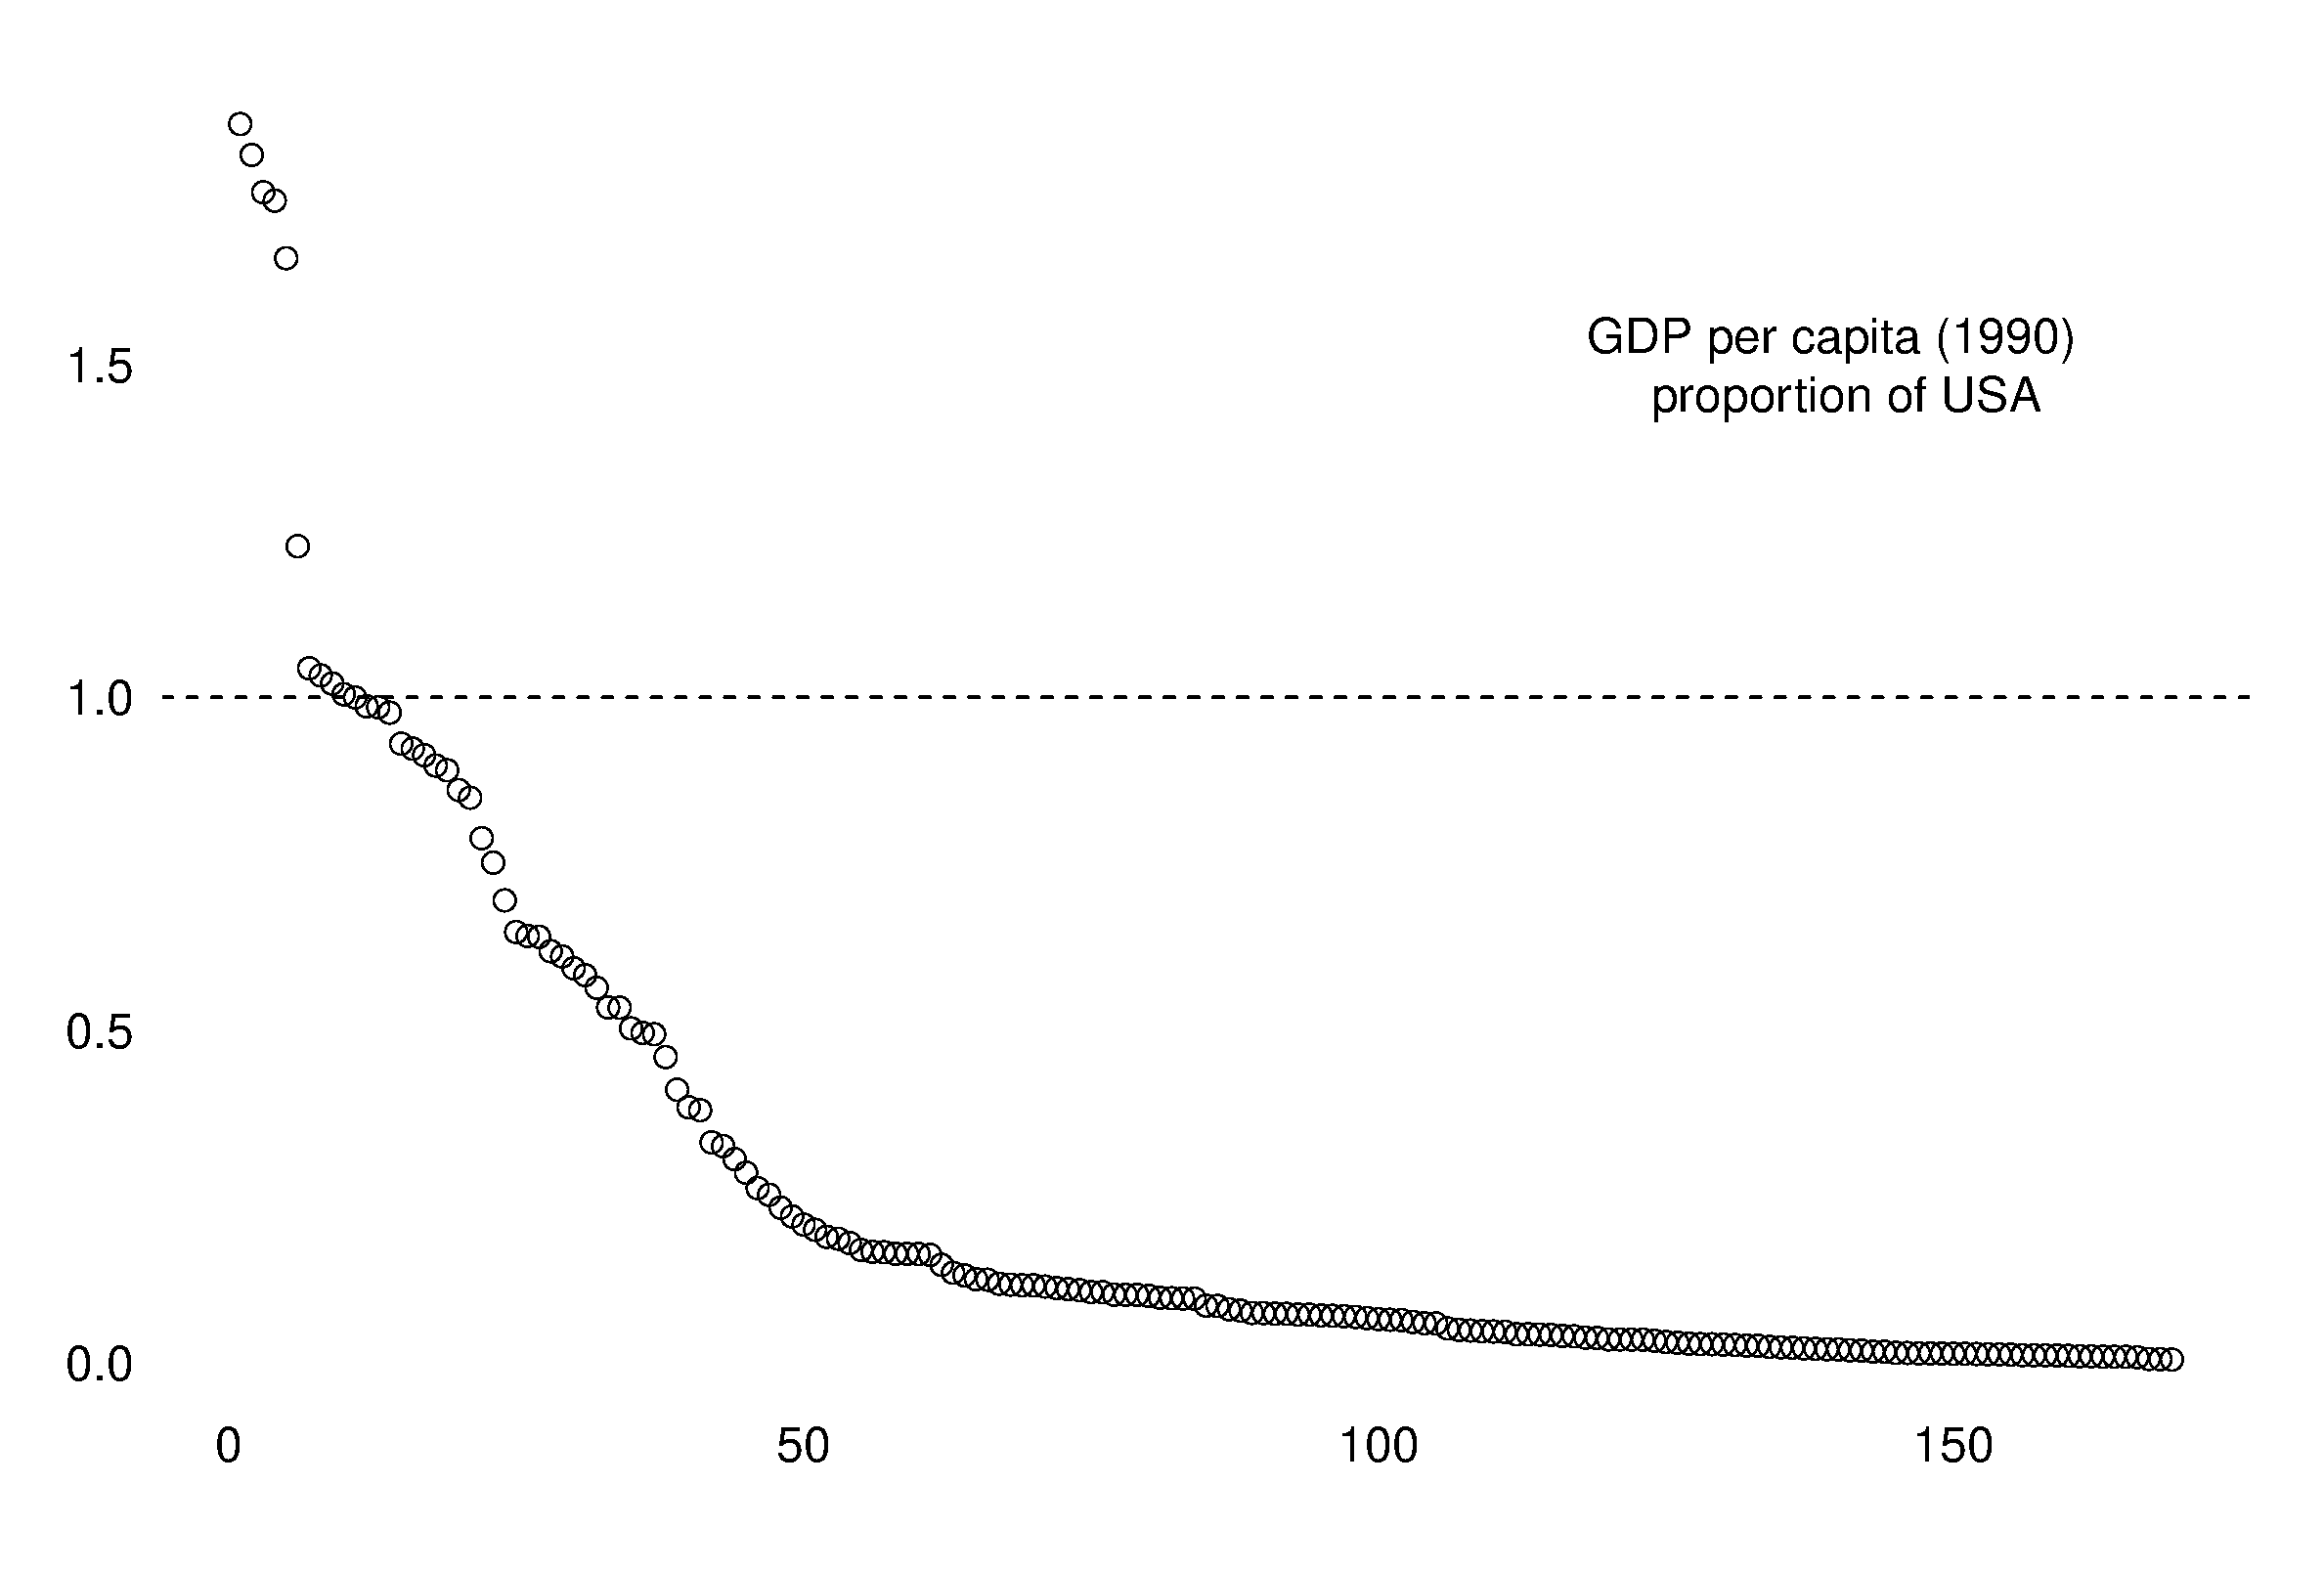
\includegraphics[scale=.2]{gdp_proportion.eps}
 \end{figure}
\end{frame}
%--------------------------------------

%--------------------------------------
\begin{frame}
  Developing countries tend to be lacking in
  \begin{itemize}
    \item Capital, both physical and human
    \item Infrastructure
    \item Technology
    \item Markets
  \end{itemize}
  \medskip
  Additionally they tend to be hampered by lack of economic freedom such as rule of law, government transparency etc. 
\end{frame}
%--------------------------------------

%--------------------------------------
\begin{frame}
 Developing countries do tend to have
 \begin{itemize}
   \item Overpopulation
   \item High inflation
   \item Corruption
   \item High mortality rates
 \end{itemize}
 And in addition they tend to be reliant on primary commodity exports. 
\end{frame}
%--------------------------------------

%--------------------------------------
\begin{frame}
 \begin{figure}
   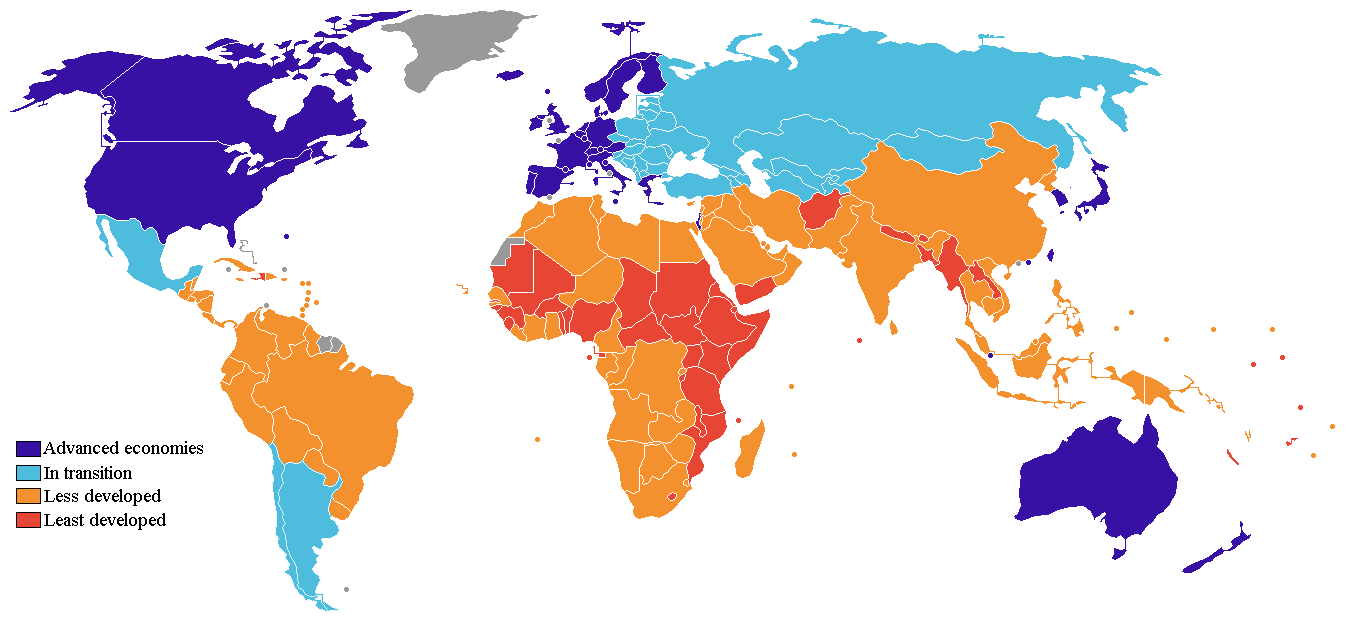
\includegraphics[scale=.3]{devcountries.png}
 \end{figure}
\end{frame}
%--------------------------------------

%--------------------------------------
\begin{frame}{Corruption index}\framesubtitle{source Transparency International}
  \begin{figure}
    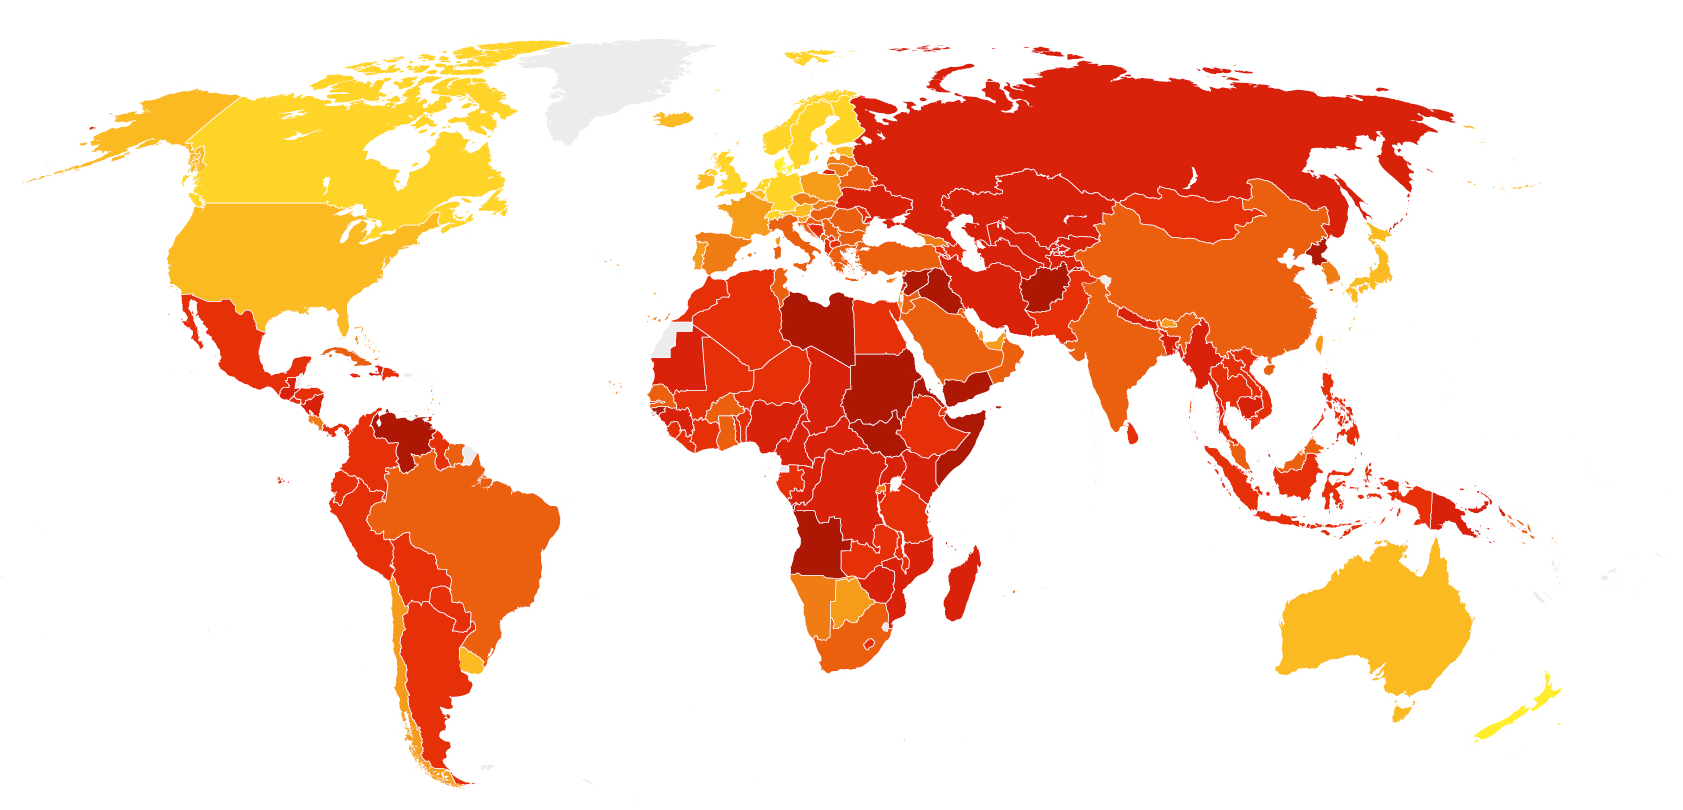
\includegraphics[scale=.3]{corruption.png}
  \end{figure}
\end{frame}
%--------------------------------------

%--------------------------------------
\begin{frame}
 The volume of international trade is actually lower than what would be predicted by trade models. 
 \begin{itemize}
   \item Trade flows are particularly small in low-income countries
 \end{itemize}
 \medskip
 This could be due to corruption which means that some trade flows go unreported, however the effect of corruption is ambiguous
 \begin{enumerate}
   \item Bribing acts as an additional tax to trade
   \item Corruption can help overcome bureaucratic barriers to trade
 \end{enumerate}
\end{frame}
%--------------------------------------

%--------------------------------------
\begin{frame}{Main export per country}\framesubtitle{source Global post}
  \begin{figure}
    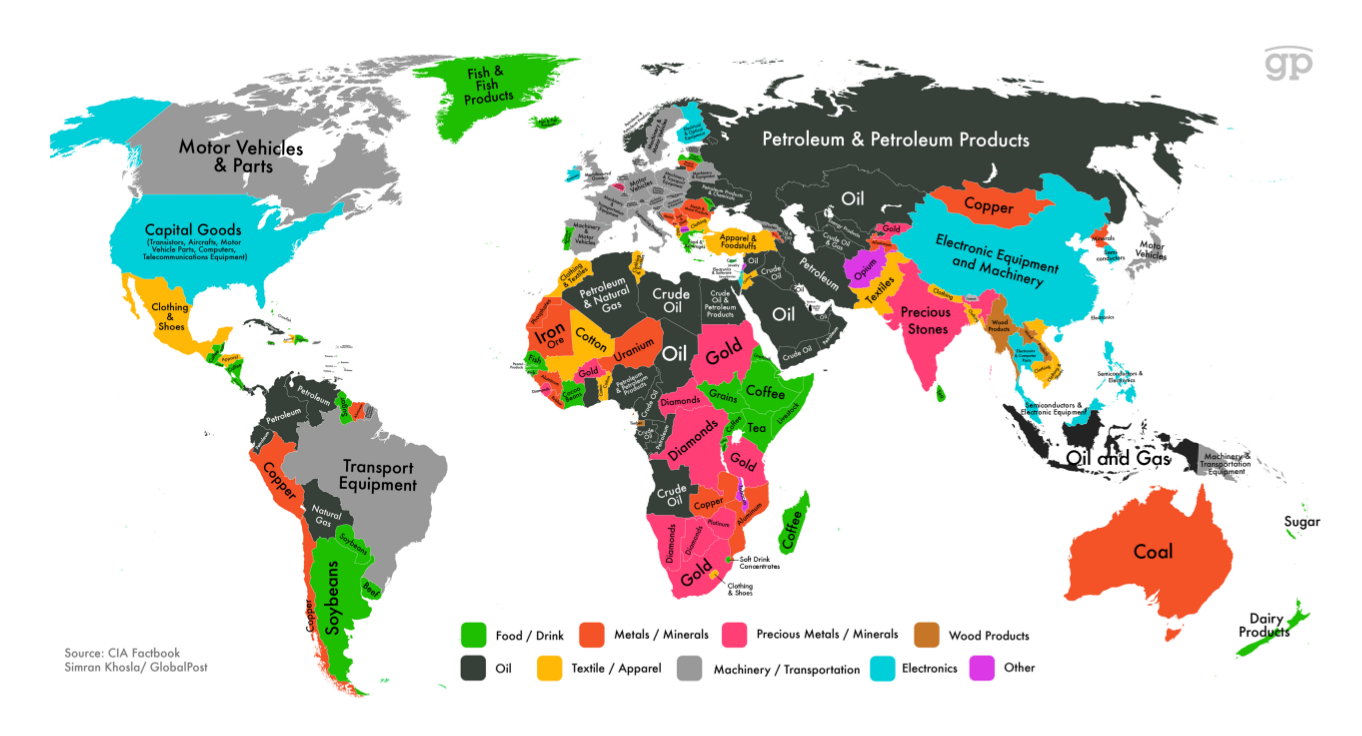
\includegraphics[scale=.9]{main_export.png}
  \end{figure}
\end{frame}
%--------------------------------------



%--------------------------------------
\begin{frame}
  \begin{figure}
    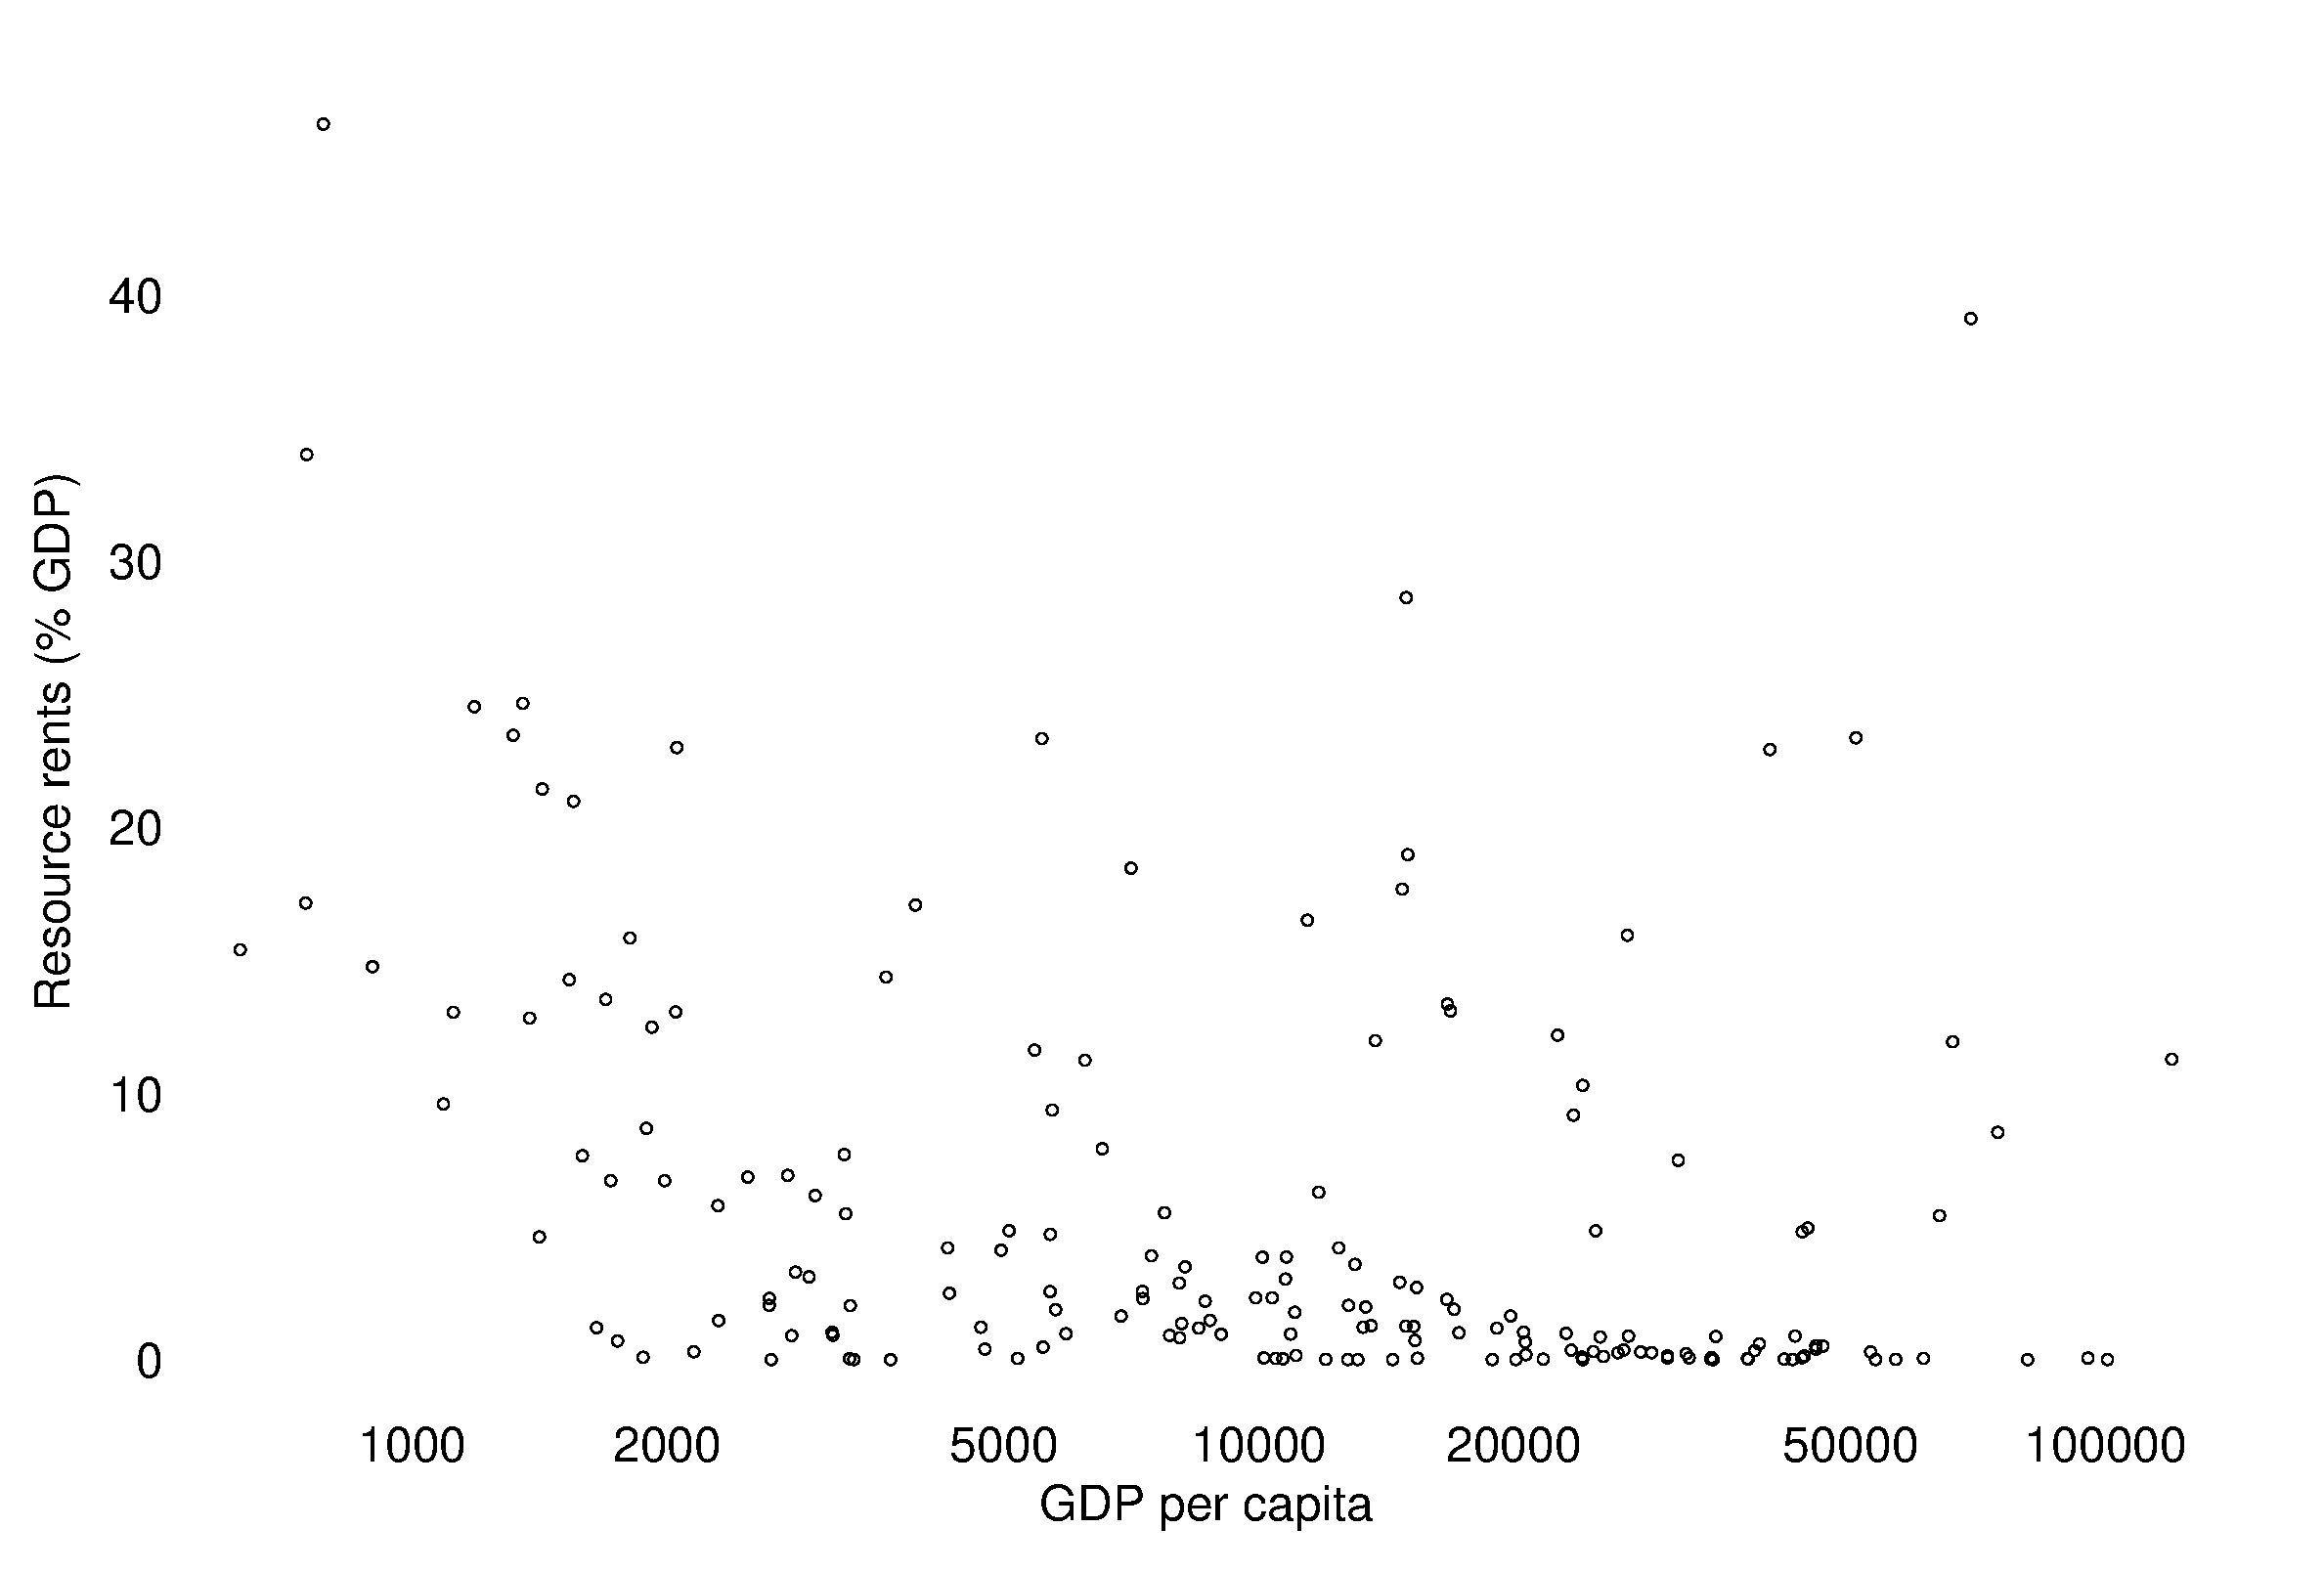
\includegraphics[scale=.3]{resource_rents.eps}
  \end{figure}
\end{frame}
%--------------------------------------


%--------------------------------------
\begin{frame}
 Developing countries rely heavily on the exports of primary commodity exports. 
 This is a problem however due to the \textbf{Prebisch-Singer hypothesis} which states that
 \medskip

 \begin{quote}
   Price of primary commodities declines over time relative to the price of manufactured goods.
 \end{quote}
 \medskip
 Manufactured goods have greater income elasticity of demand compared to primary products such as foodstuffs.
\end{frame}
%--------------------------------------

%--------------------------------------
\begin{frame}
  The Prebisch-Singer hypothesis predicts that commodity prices will follow a downward trend, but the evidence for this stylised fact is very mixed
  \begin{enumerate}
    \item There is a negative downward trend in price time-series of main commodities
    \item Others noticed an increase in commodity prices since the 1950s
  \end{enumerate}
  \medskip
  It seems that the hypothesis holds for some commodities but that there is no general effect.
\end{frame}
%--------------------------------------

%--------------------------------------
\begin{frame}
  \begin{figure}
    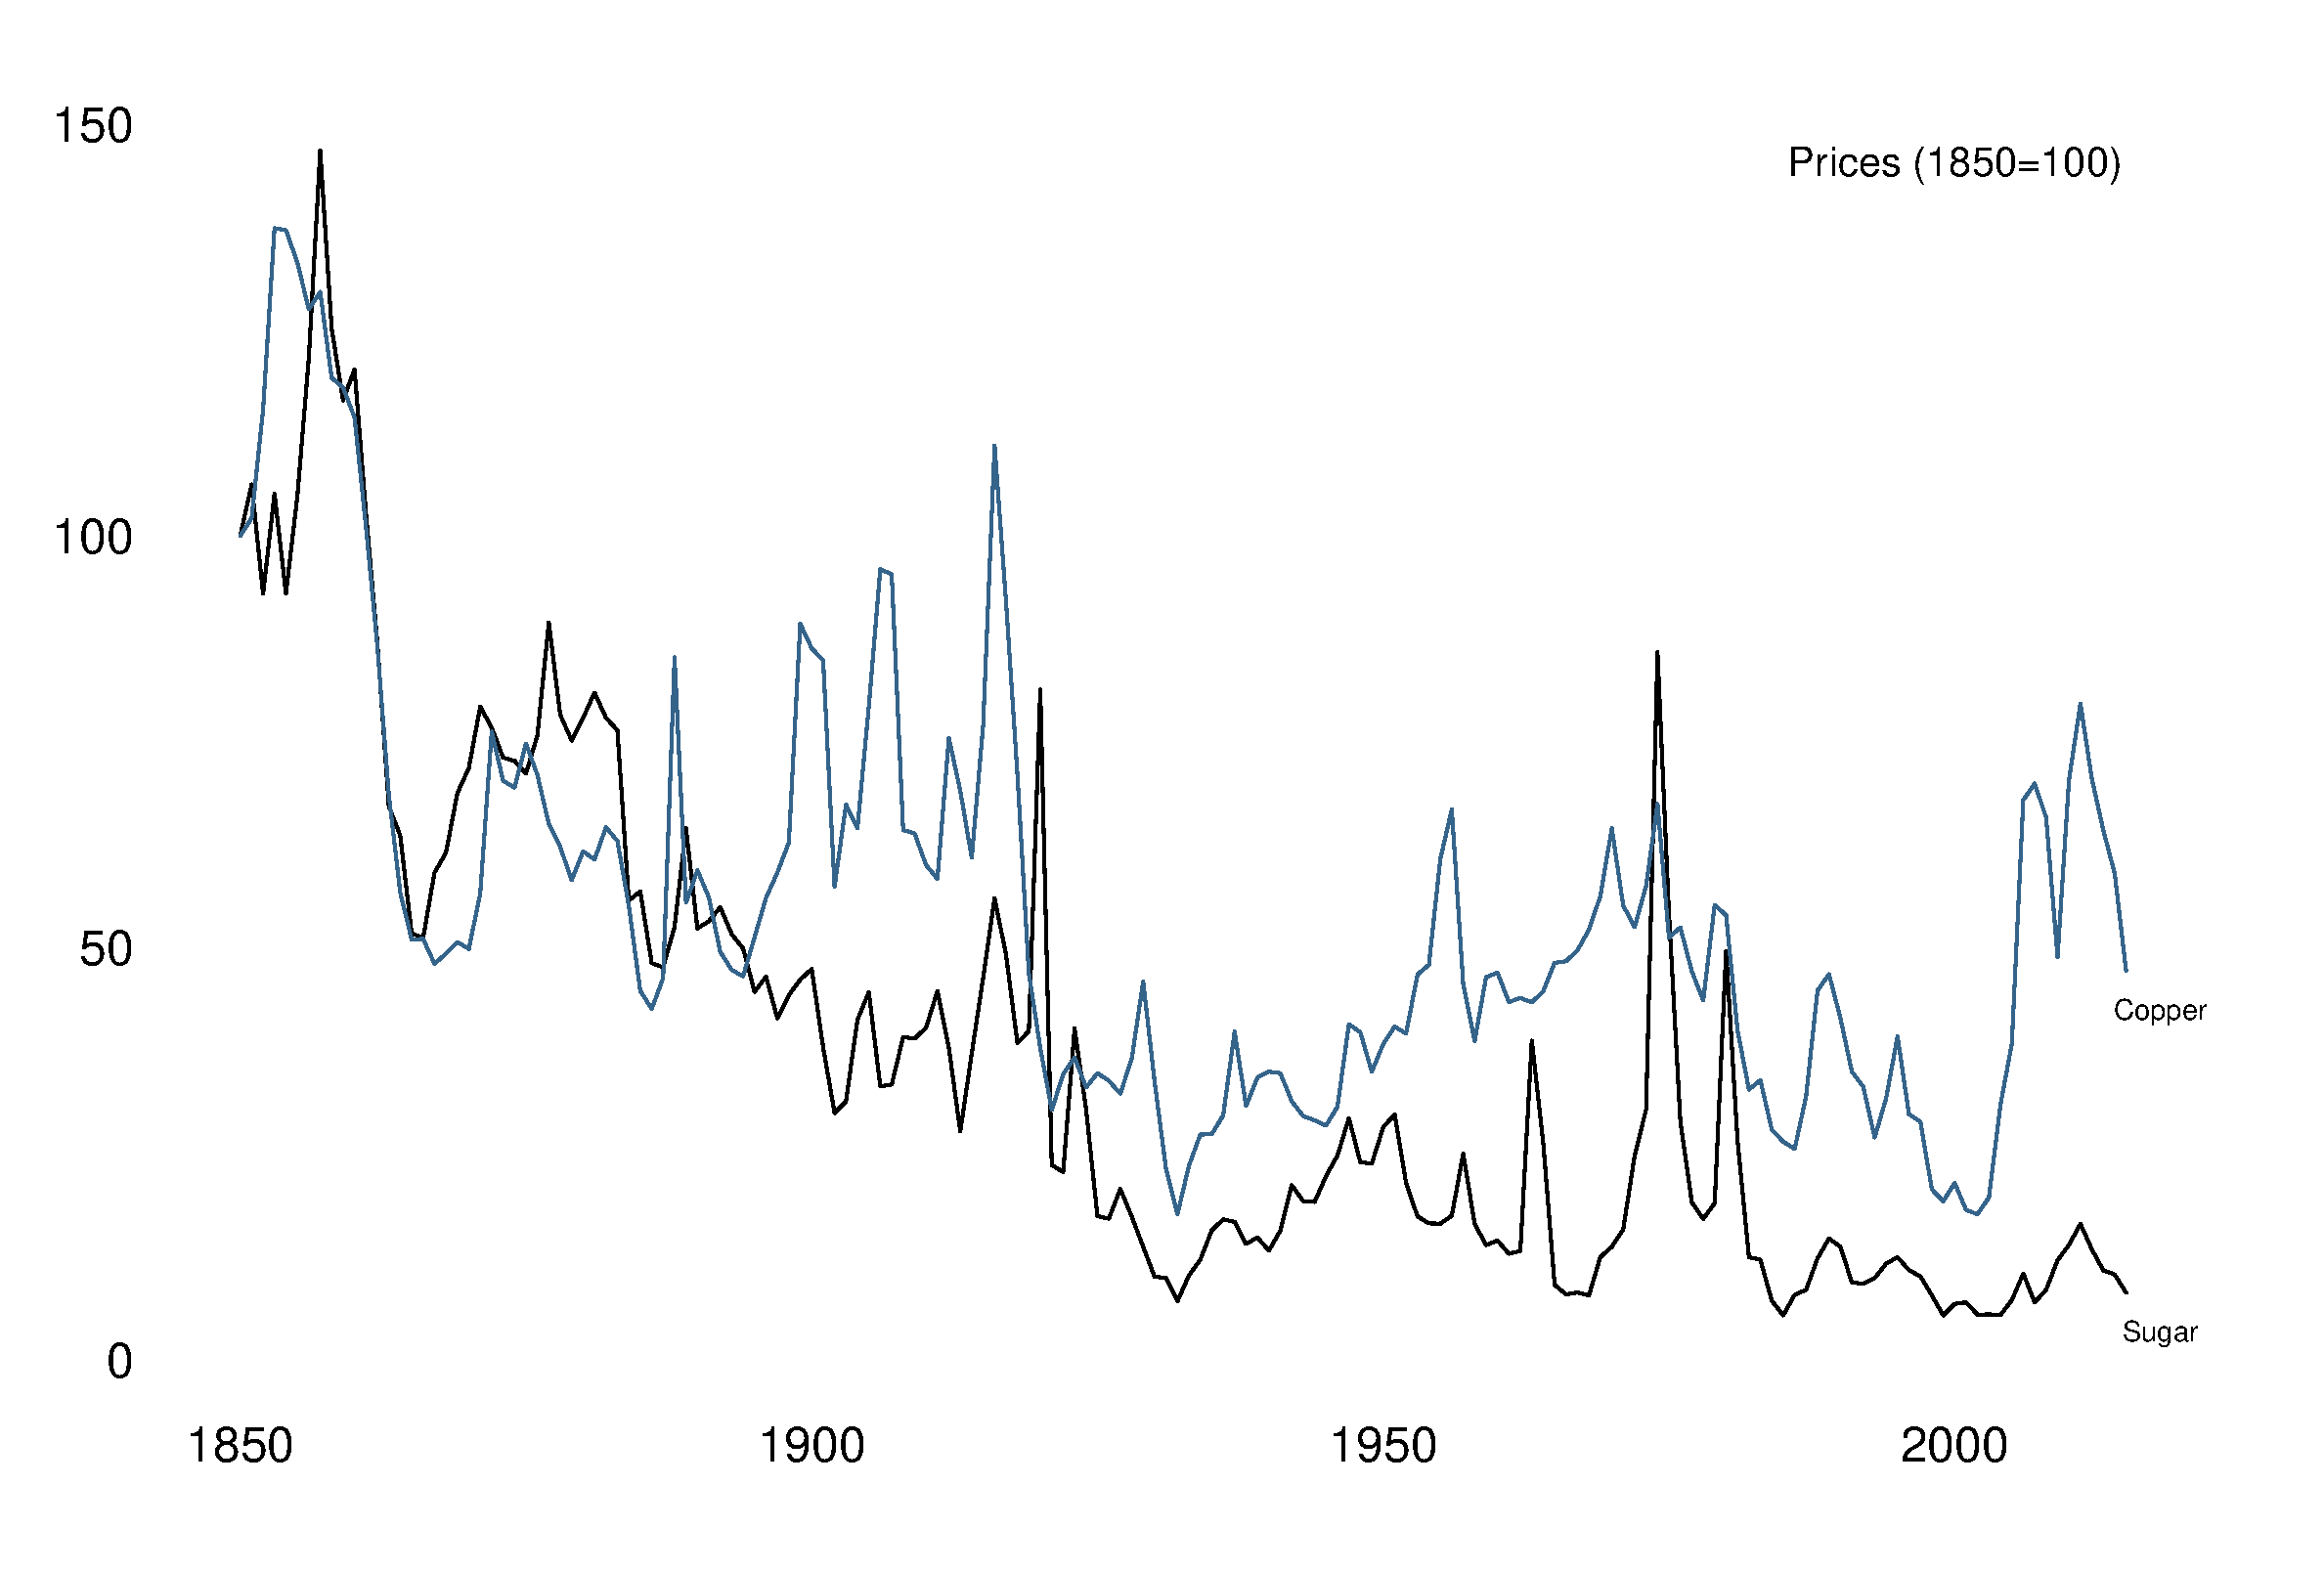
\includegraphics[scale=.3]{commodity_prices.eps}
  \end{figure}
\end{frame}
%--------------------------------------

%--------------------------------------
\begin{frame}
 What are the implications of the Prebisch-Singer hypothesis for international trade and developing countries?
 One is that primary commodity prices will decline when efficiency increases
 \begin{itemize}
   \item This means that as countries start exporting, the price of primary commodities declines relative to the price of manufactured goods
 \end{itemize}
 \medskip
 This means that there is a deterioration in the terms of trade for a country that relies on primary commodity exports.
 \begin{itemize}
   \item These countries should diversify their economy to become less dependent
   \item Sound advice, hard to implement (see specific-factors model)
 \end{itemize}
\end{frame}
%--------------------------------------

%--------------------------------------
\begin{frame}
  Let's look at an example; the coffee trade. 
  \begin{itemize}
    \item Coffee is primarily grown in developing countries    
  \end{itemize}
  \medskip
  Over the past two decades there have been large fluctuations in the price of coffee
\end{frame}
%--------------------------------------

%--------------------------------------
\begin{frame}
  \begin{figure}
    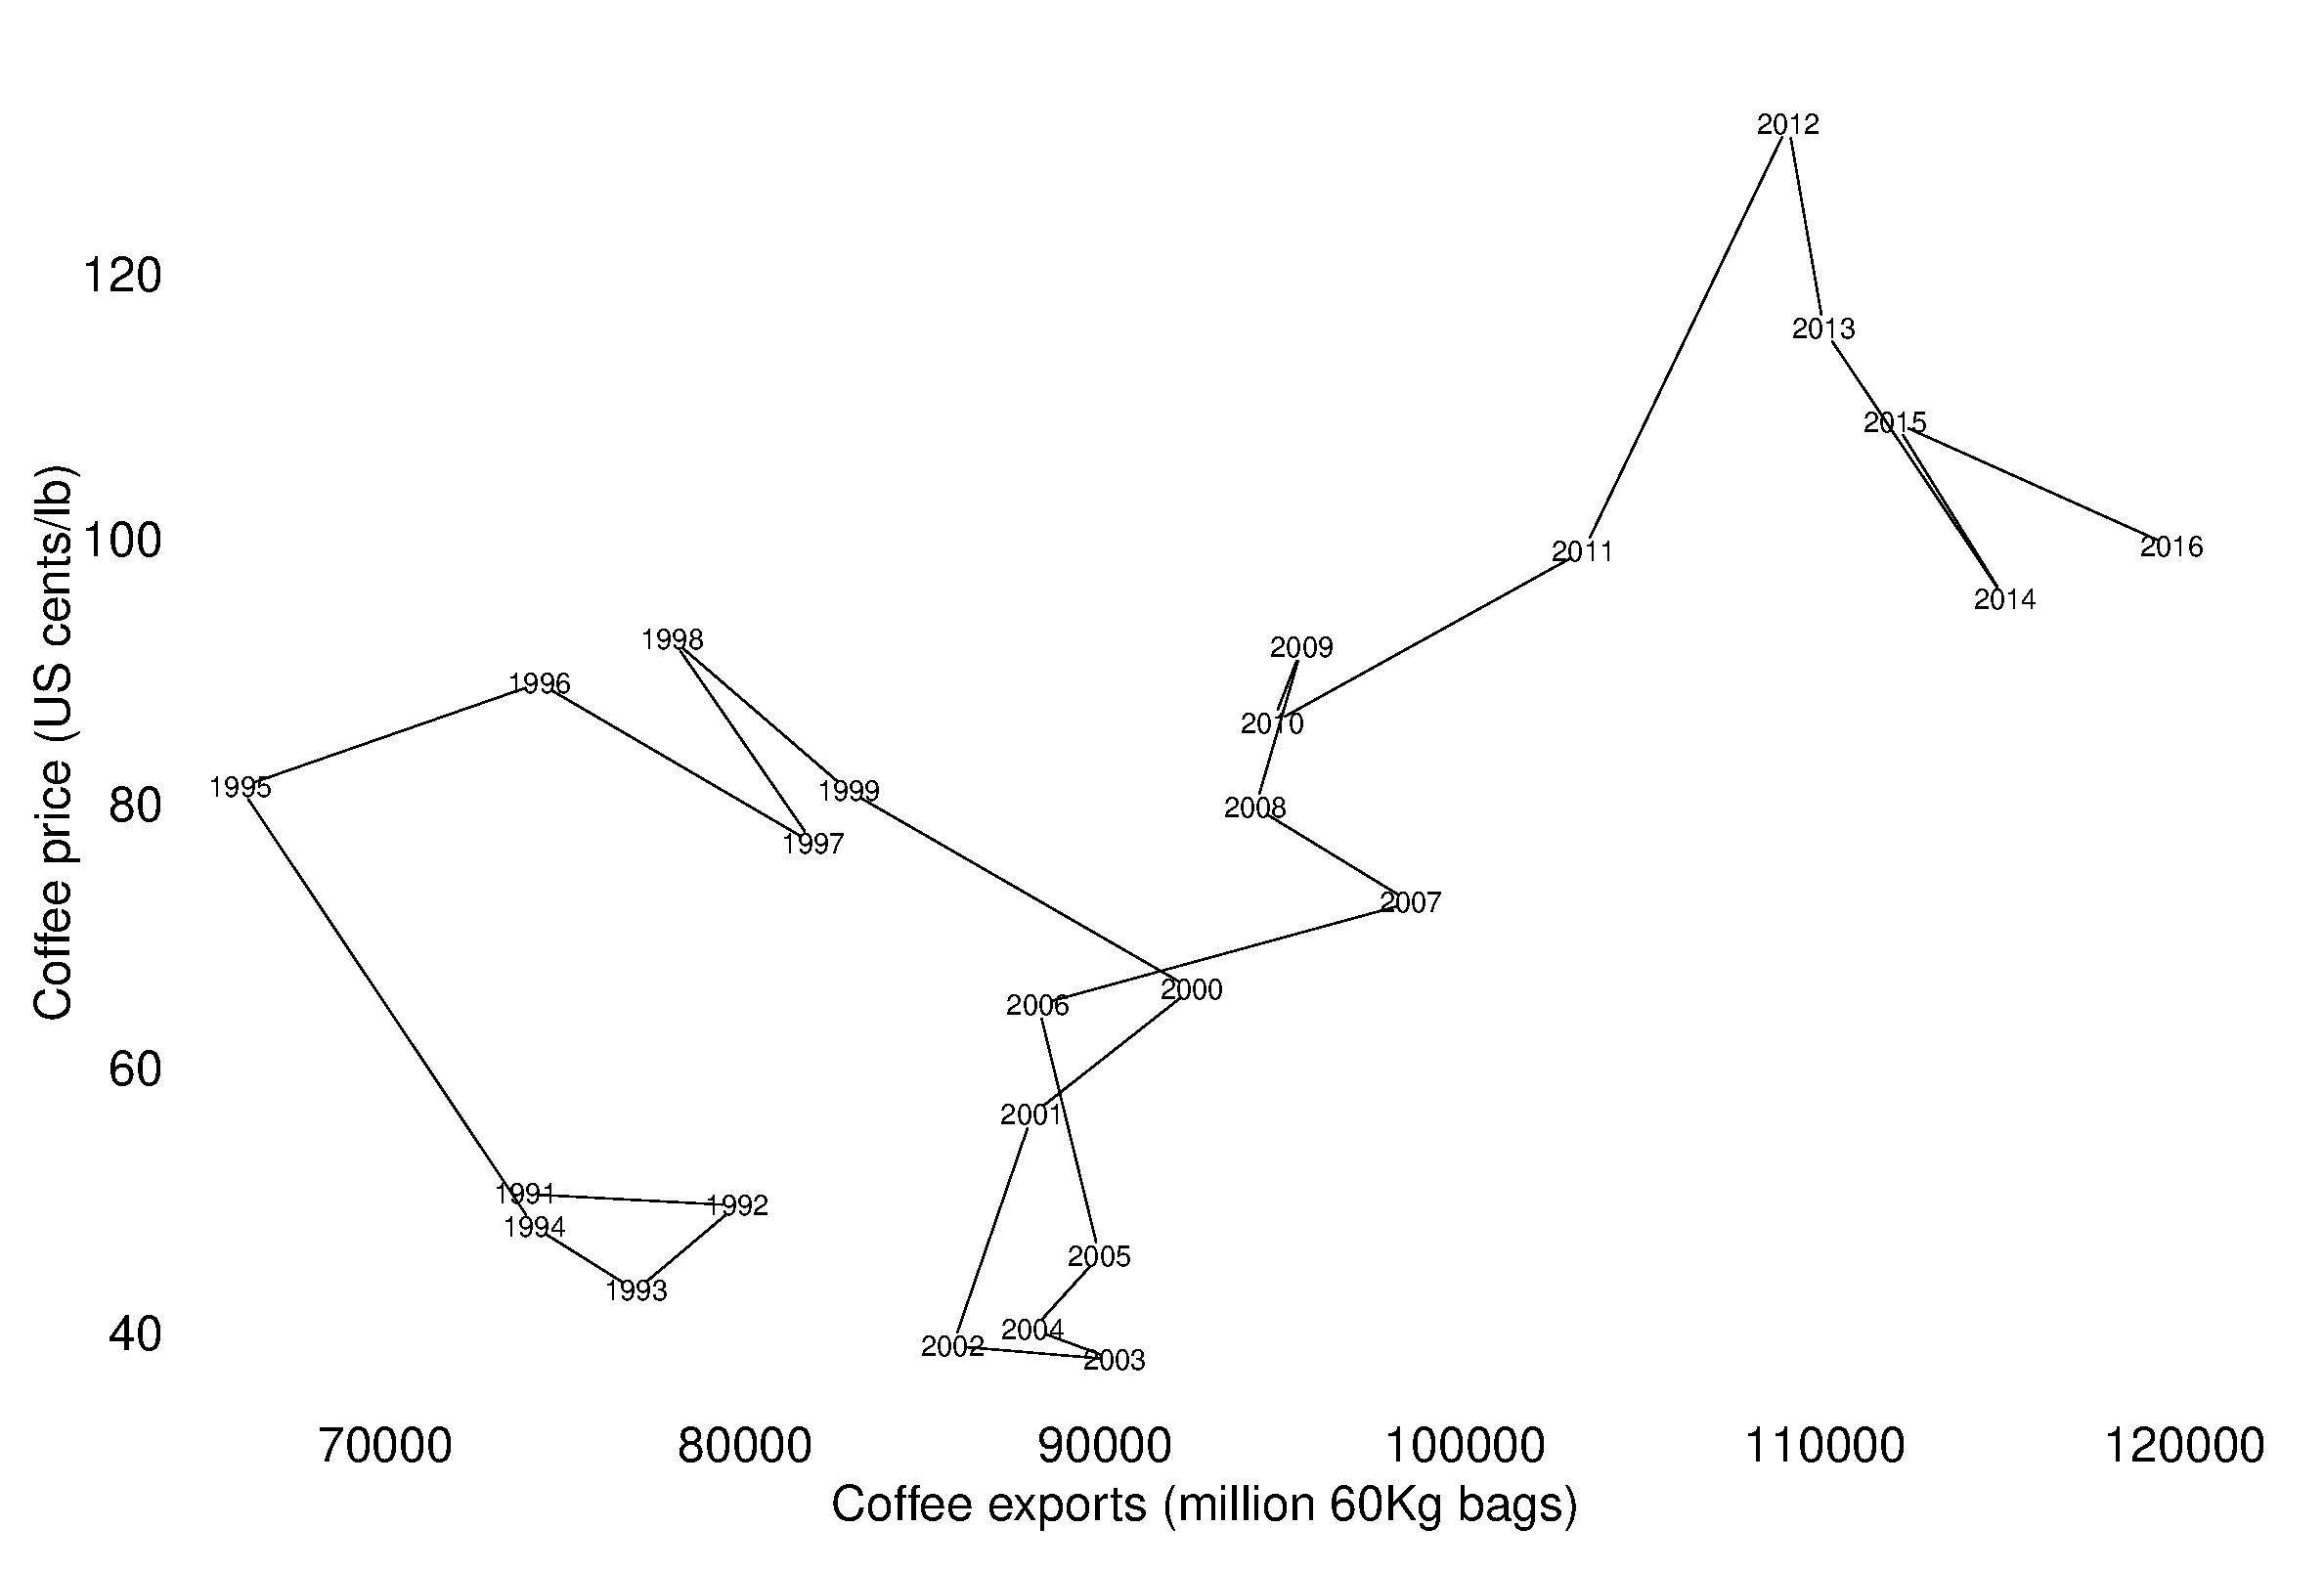
\includegraphics[scale=.3]{coffee.eps}
  \end{figure}
\end{frame}
%--------------------------------------

%--------------------------------------
\begin{frame}
  \begin{figure}
    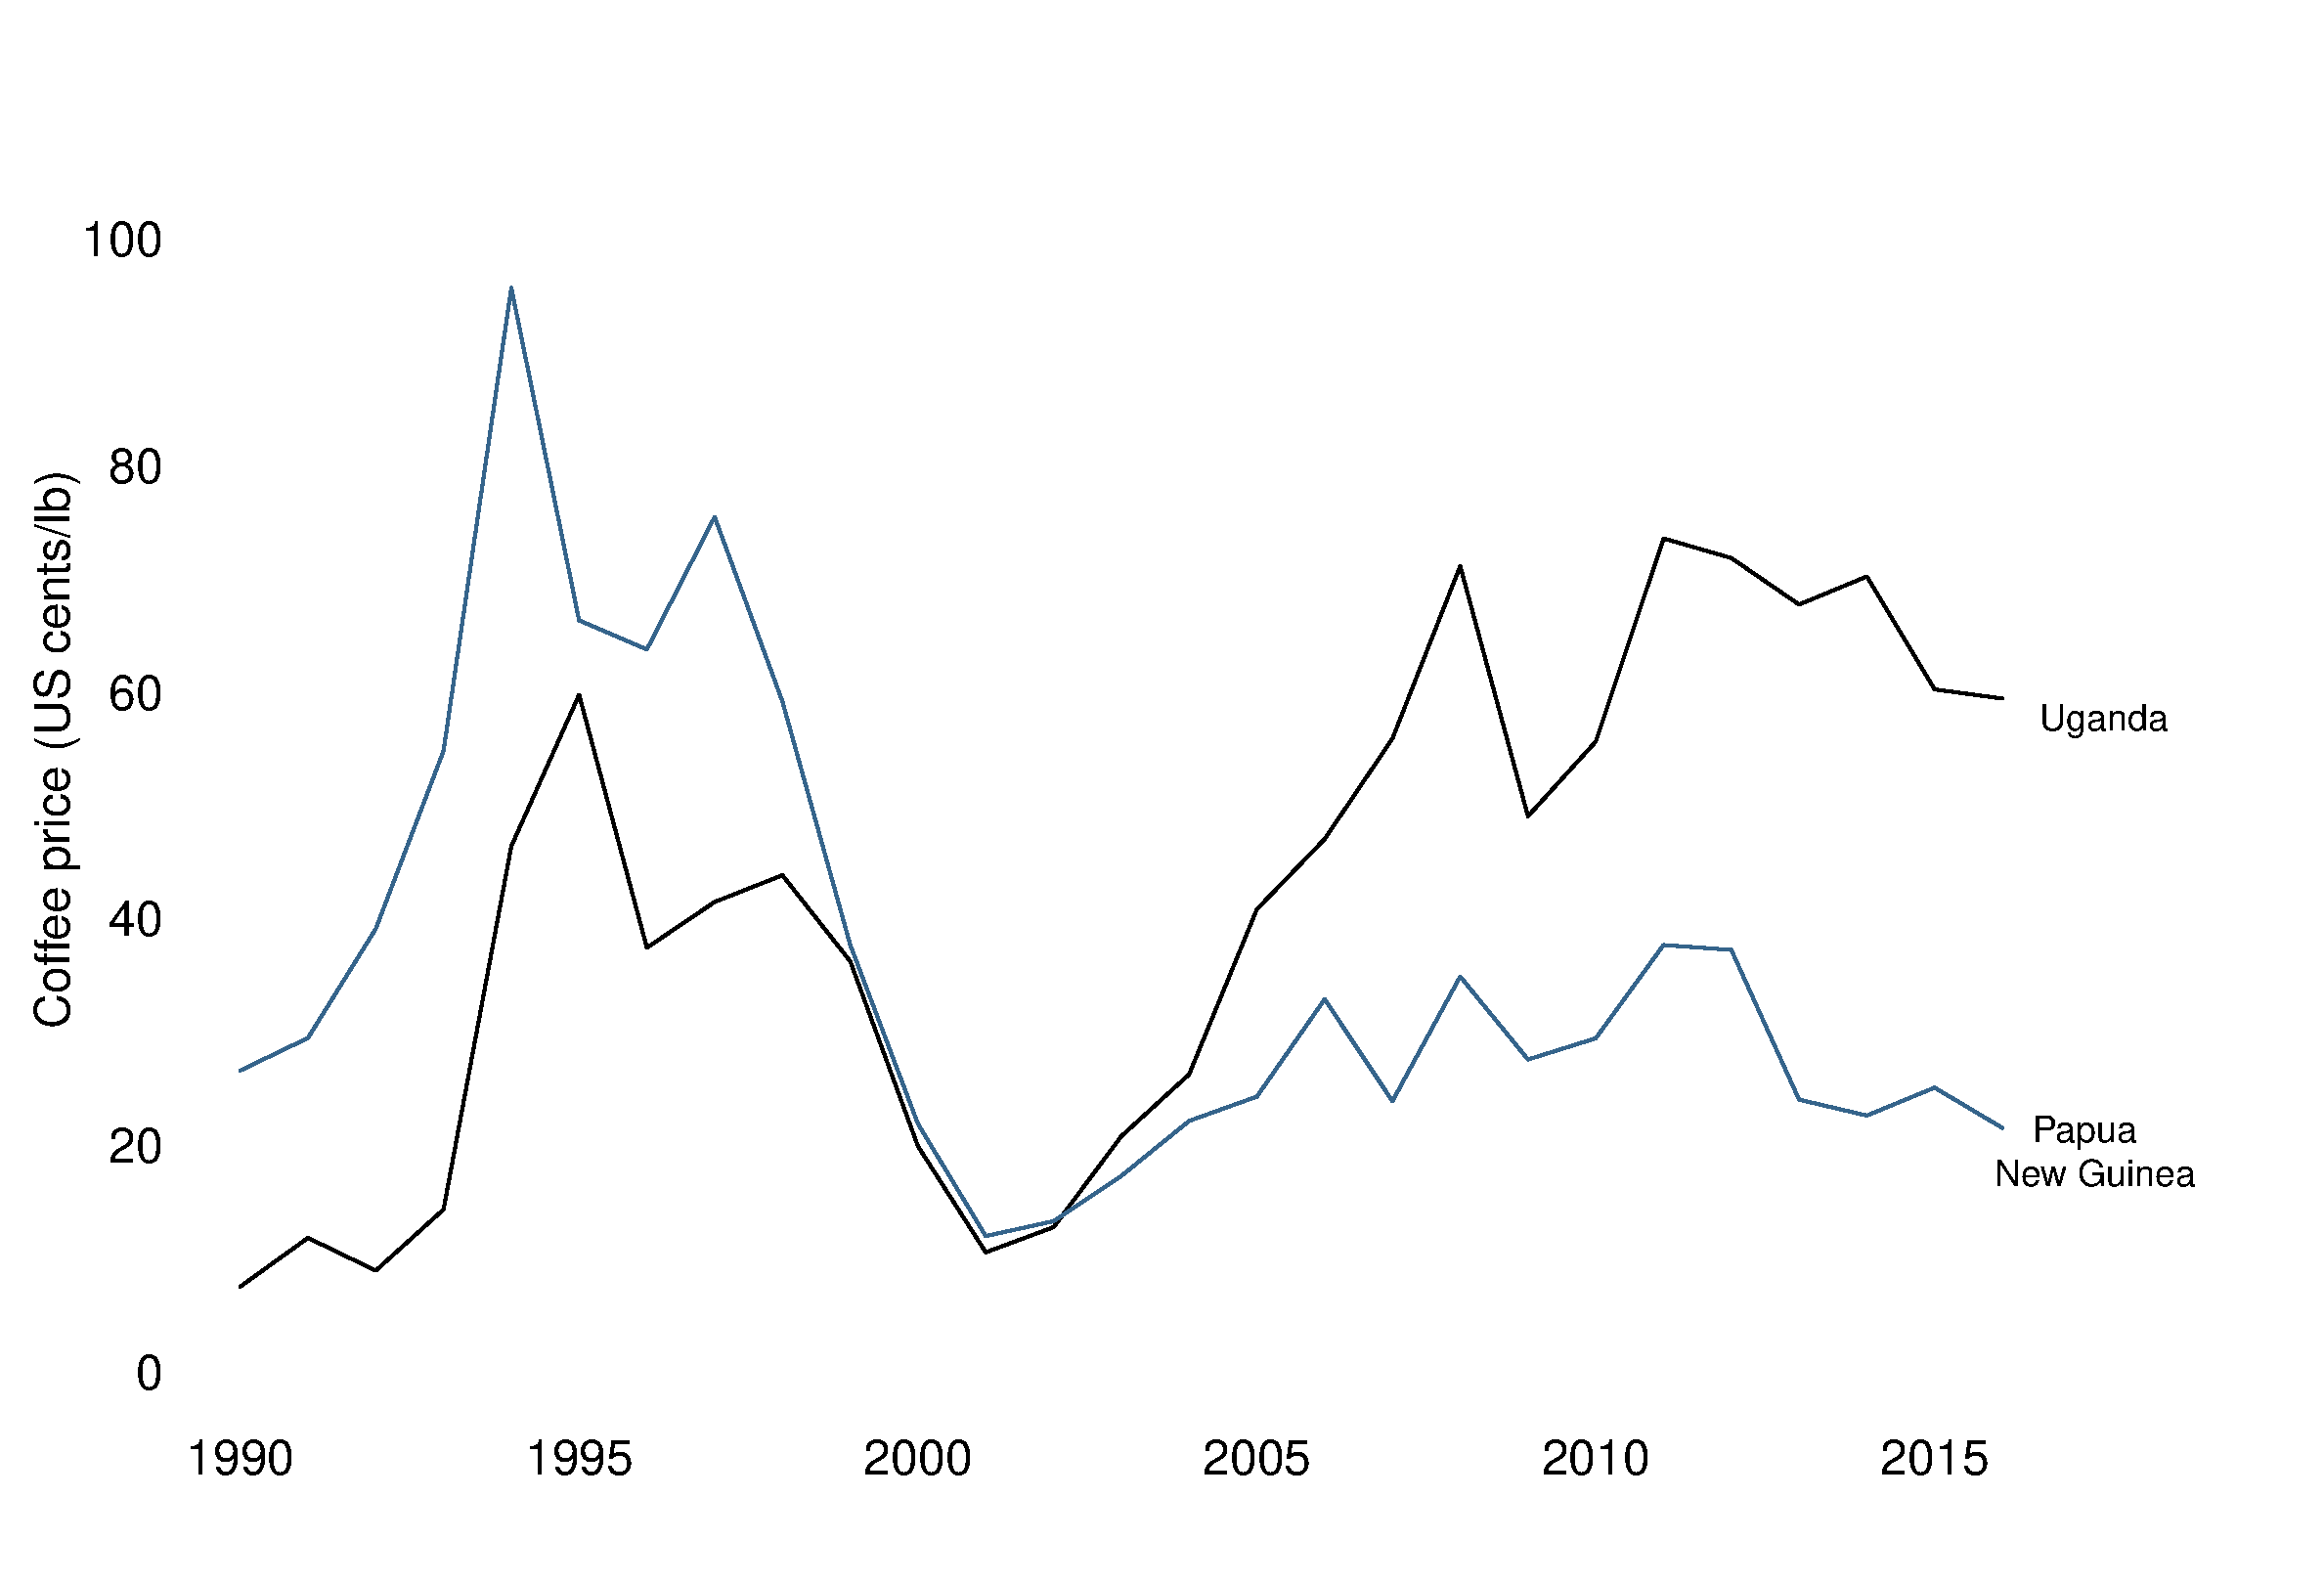
\includegraphics[scale=.3]{coffee2.eps}
  \end{figure}
\end{frame}
%--------------------------------------

%--------------------------------------
\begin{frame}
  Large price fluctuations means large fluctuations in the real income of coffee farmers.
  \begin{itemize}
    \item Government often protect the agricultural sector from the negative effects of trade
    \item Protection will increase farmer income but also raise domestic price of consumed good
  \end{itemize}
\end{frame}
%--------------------------------------

%--------------------------------------
\begin{frame}
  Dube \& Vargas (2013) examine relation between commodity prices and conflict on Colombia focusing on coffee and oil
  \medskip
  \begin{itemize}
    \item Coffee is labour-intensive; positive price shock will increase wages and lower opportunity costs for conflict
    \item Oil is capital-intensive: positive price shock will increase rents, stimulating rent-seeking making conflict more likely
  \end{itemize}
\end{frame}
%--------------------------------------


%--------------------------------------
\begin{frame}
  \begin{figure}
    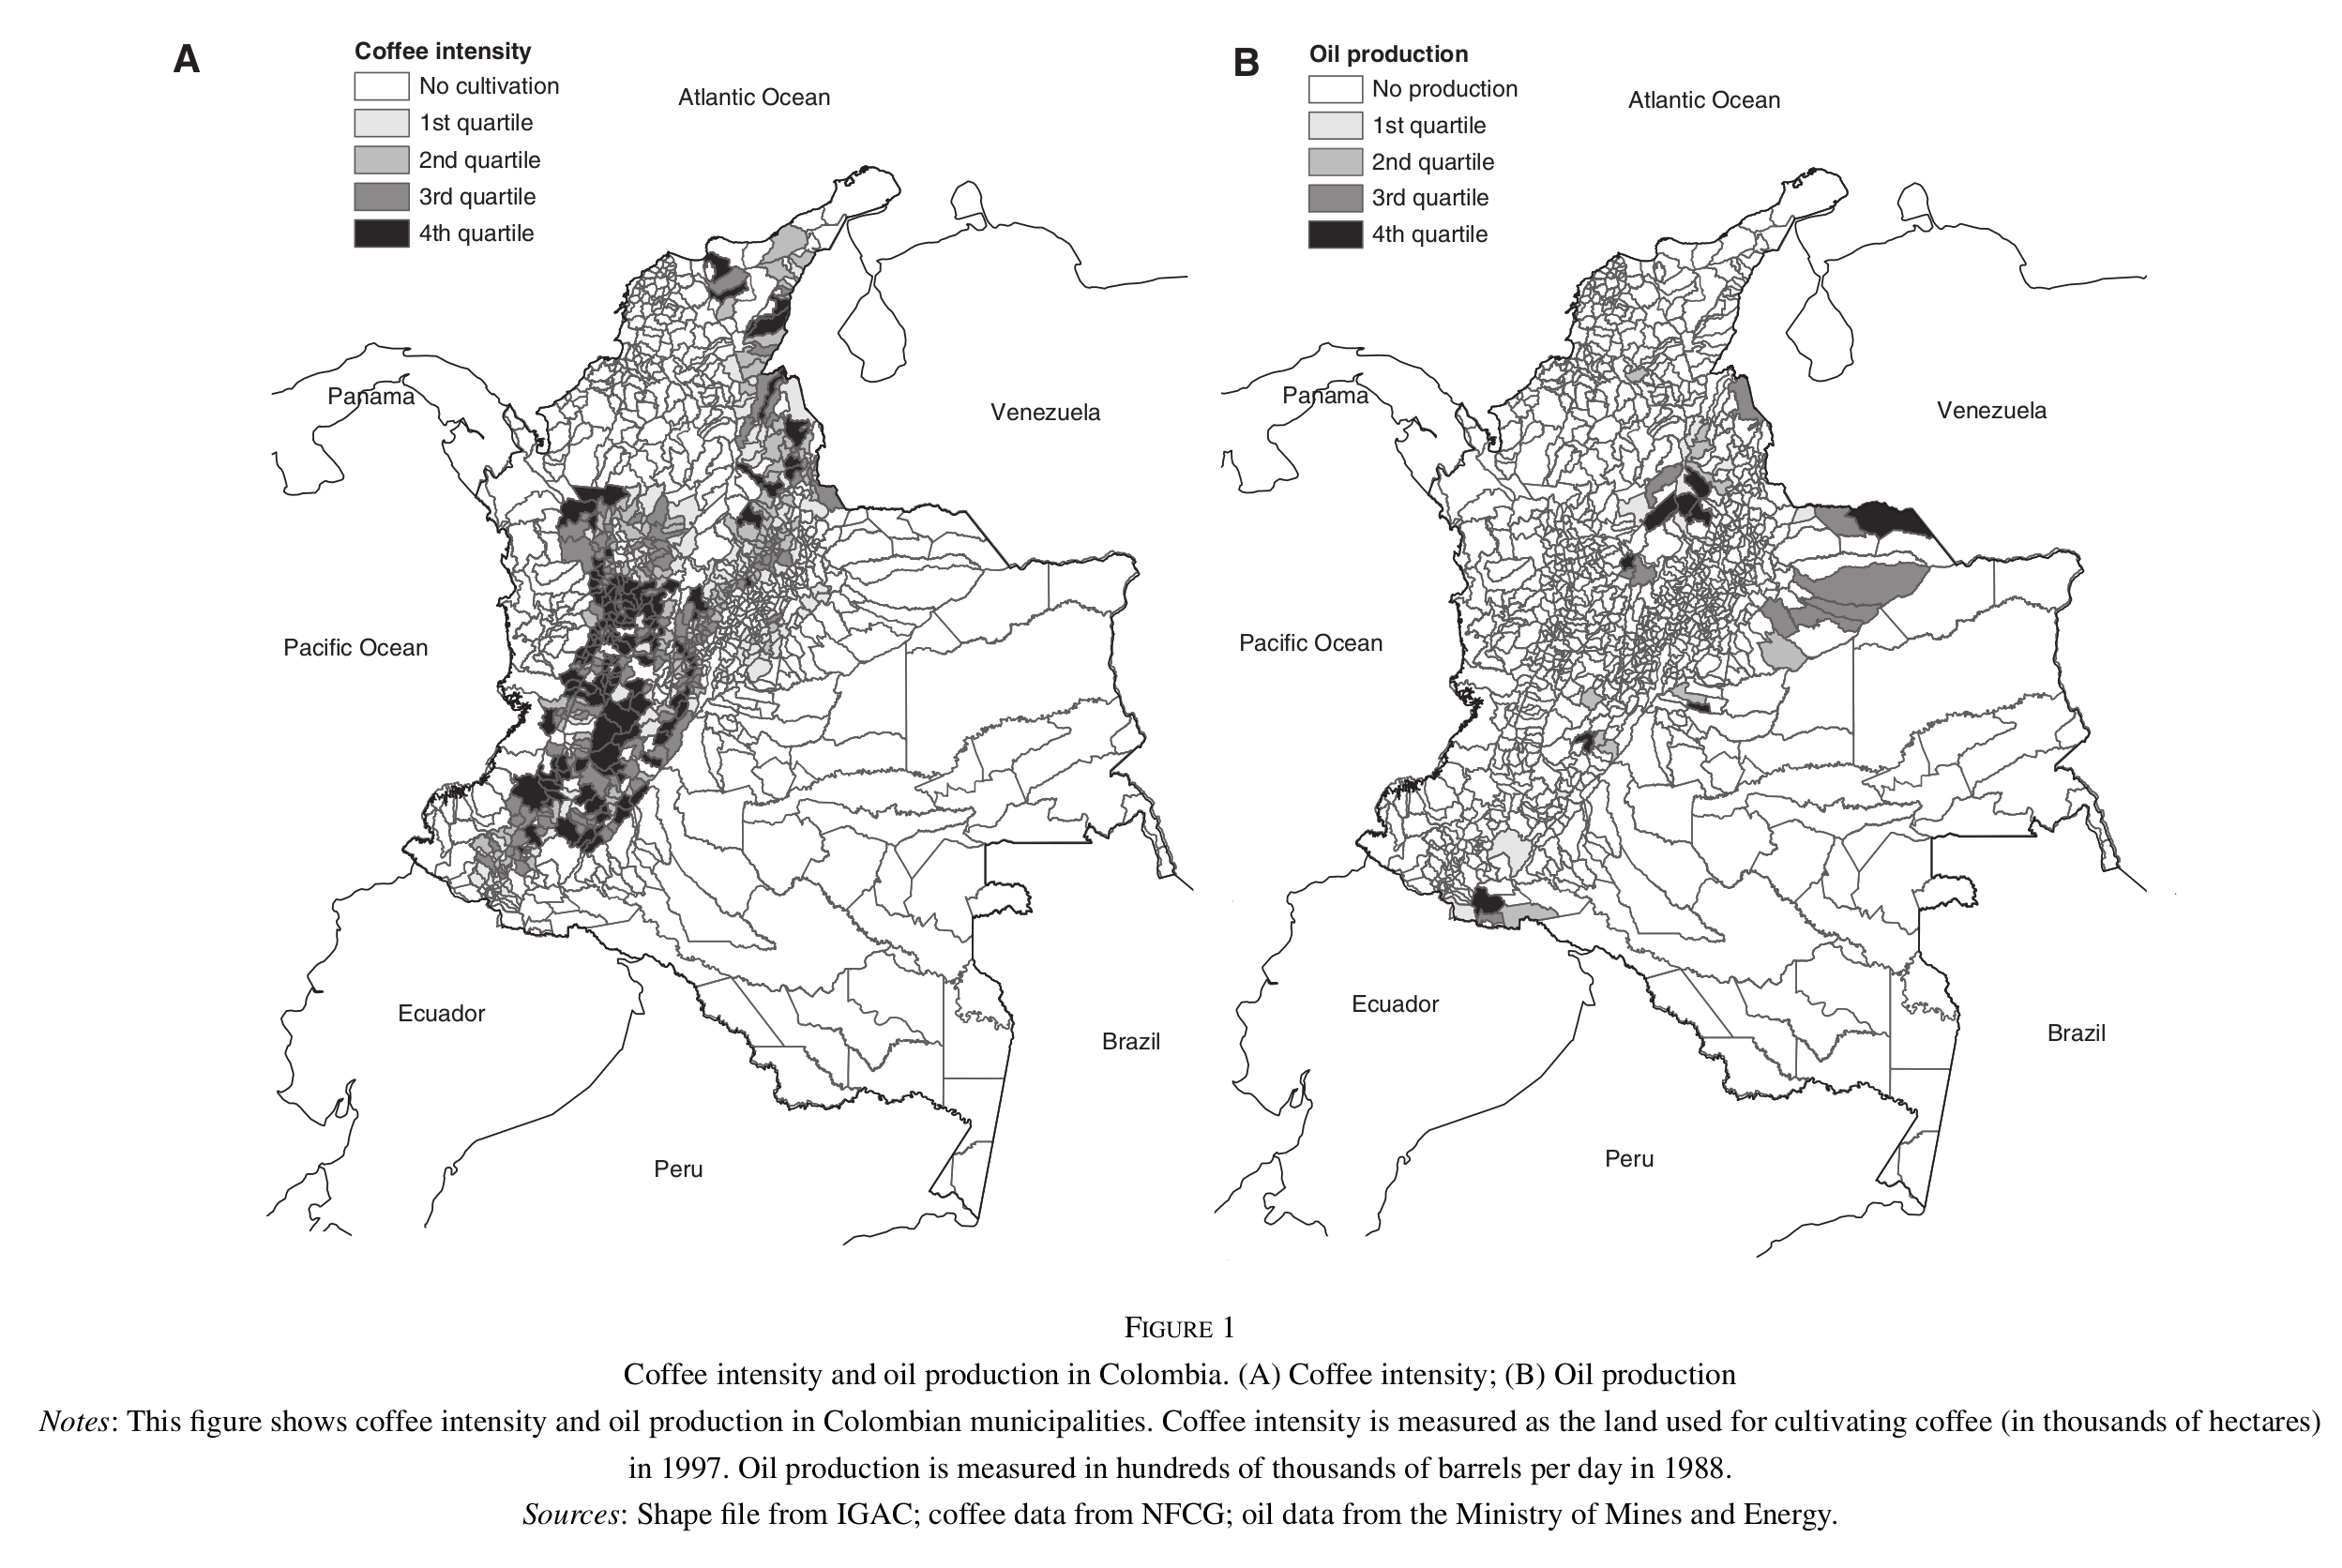
\includegraphics[scale=.55]{dube_vargas1.png}
  \end{figure}
\end{frame}
%--------------------------------------

%--------------------------------------
\begin{frame}
  \begin{figure}
    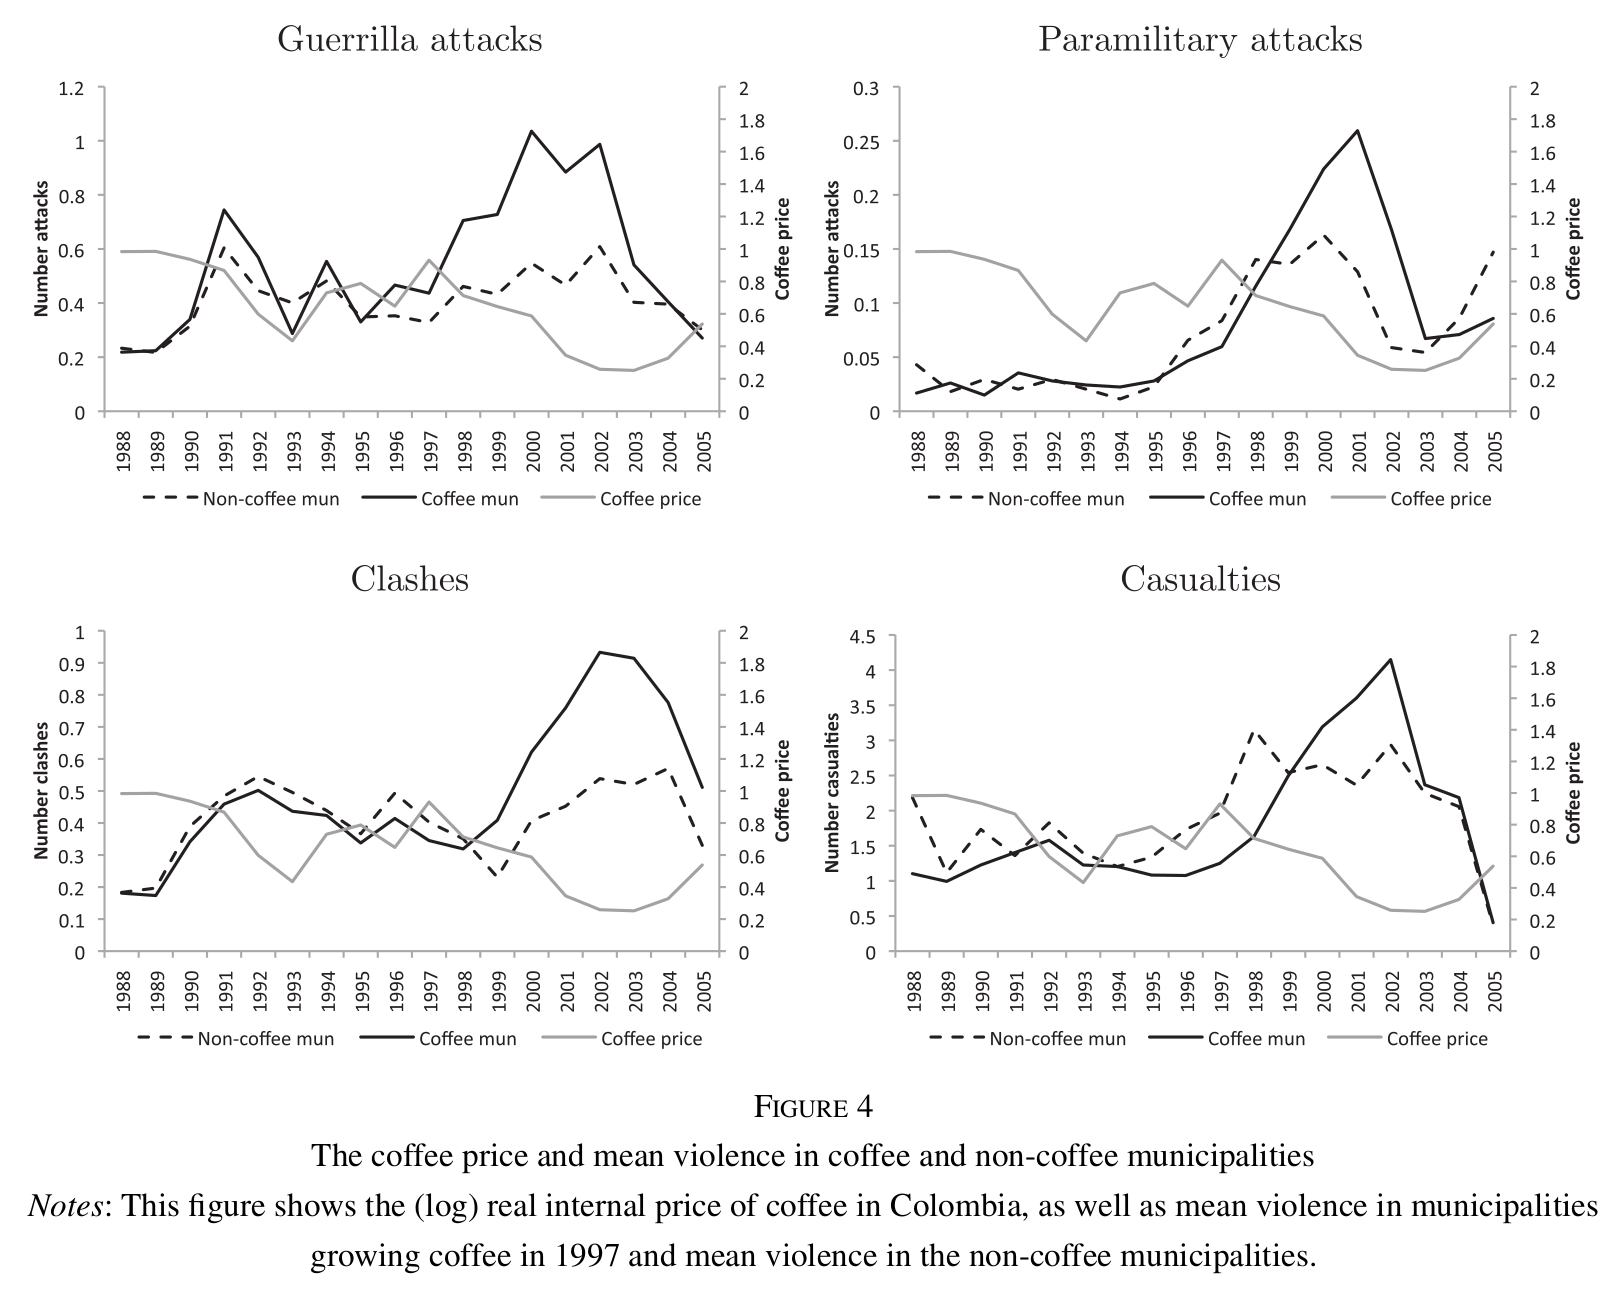
\includegraphics[scale=.6]{dube_vargas2.png}
  \end{figure}
\end{frame}
%--------------------------------------

%--------------------------------------
\begin{frame}
  \begin{figure}
    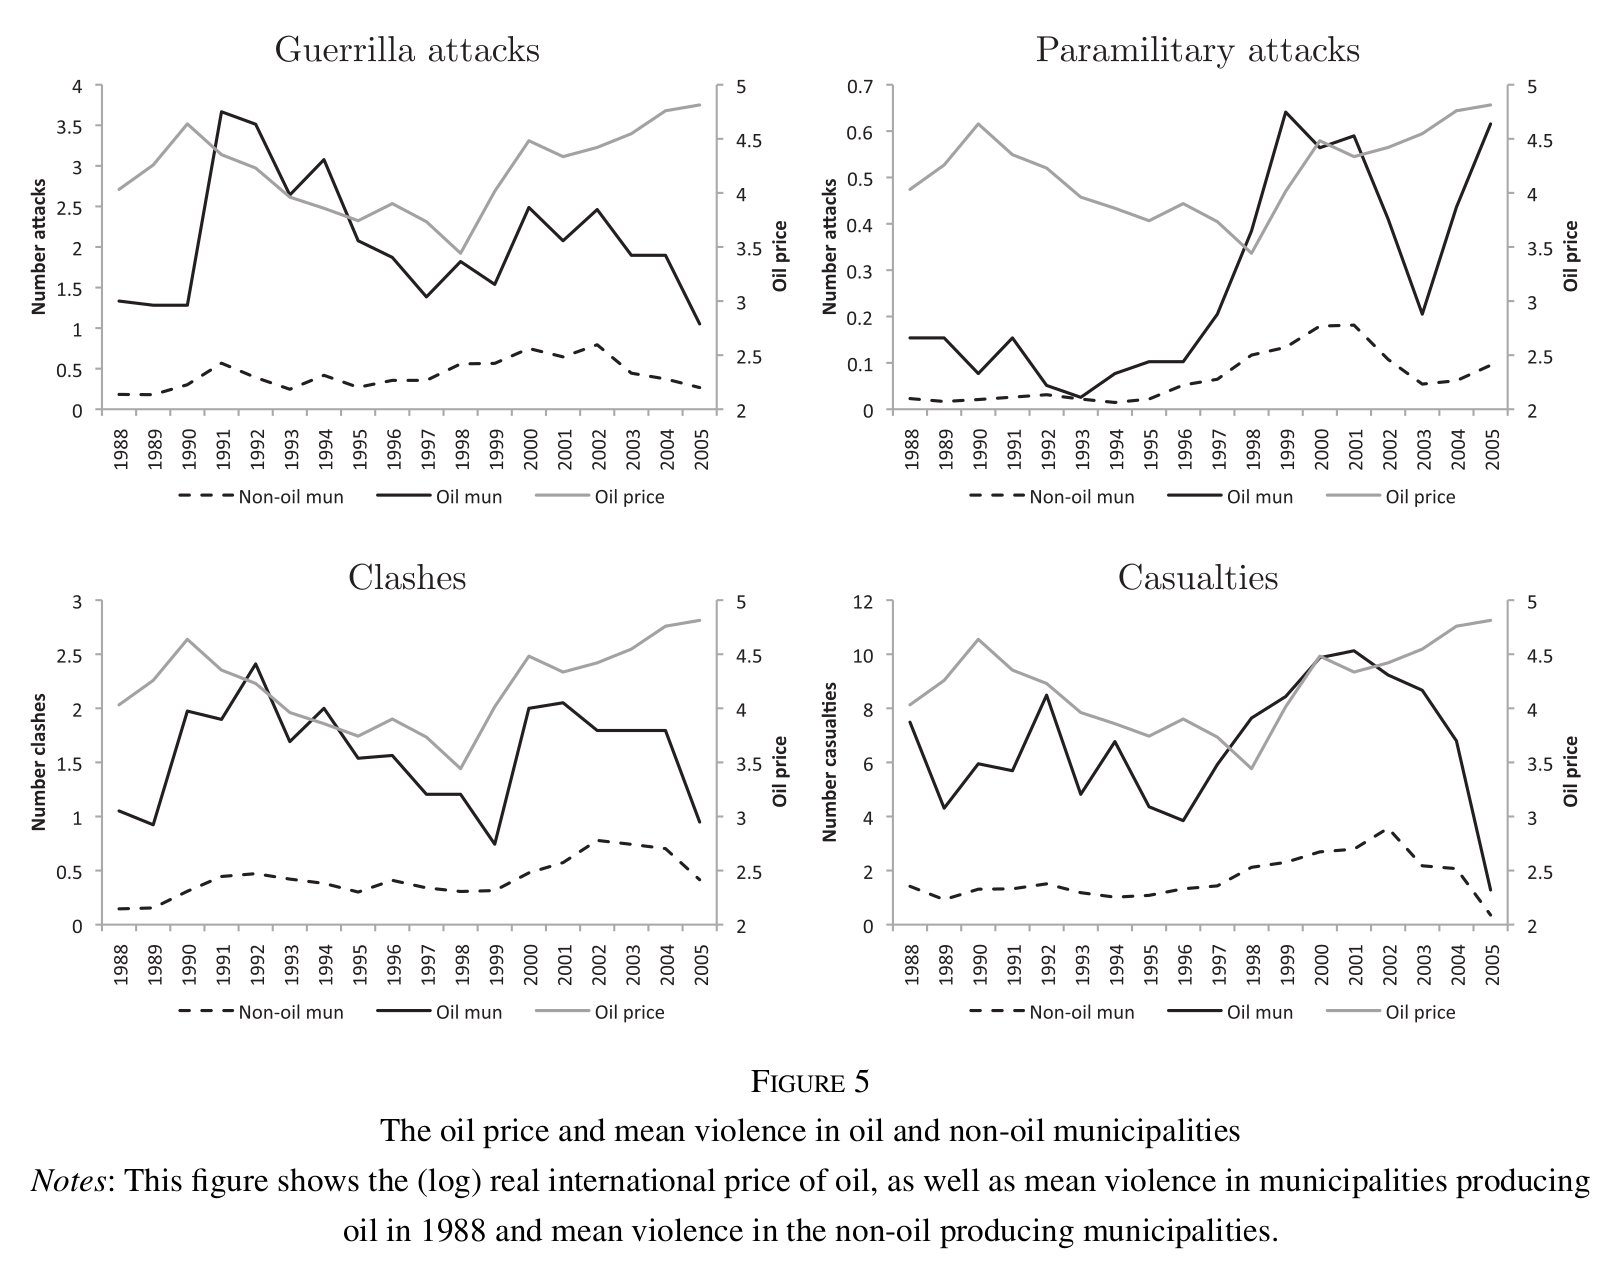
\includegraphics[scale=.6]{dube_vargas3.png}
  \end{figure}
\end{frame}
%--------------------------------------


%--------------------------------------
\begin{frame}
 Within economics there is something called the \textbf{resource curse} which is a paradox that suggests that resource-rich countries tend to grow slower and are less developed compared to resource poor countries
 \begin{itemize}
   \item Compare Denmark to the DRC
 \end{itemize}
\end{frame}
%--------------------------------------

%--------------------------------------
\begin{frame}
  \begin{figure}
    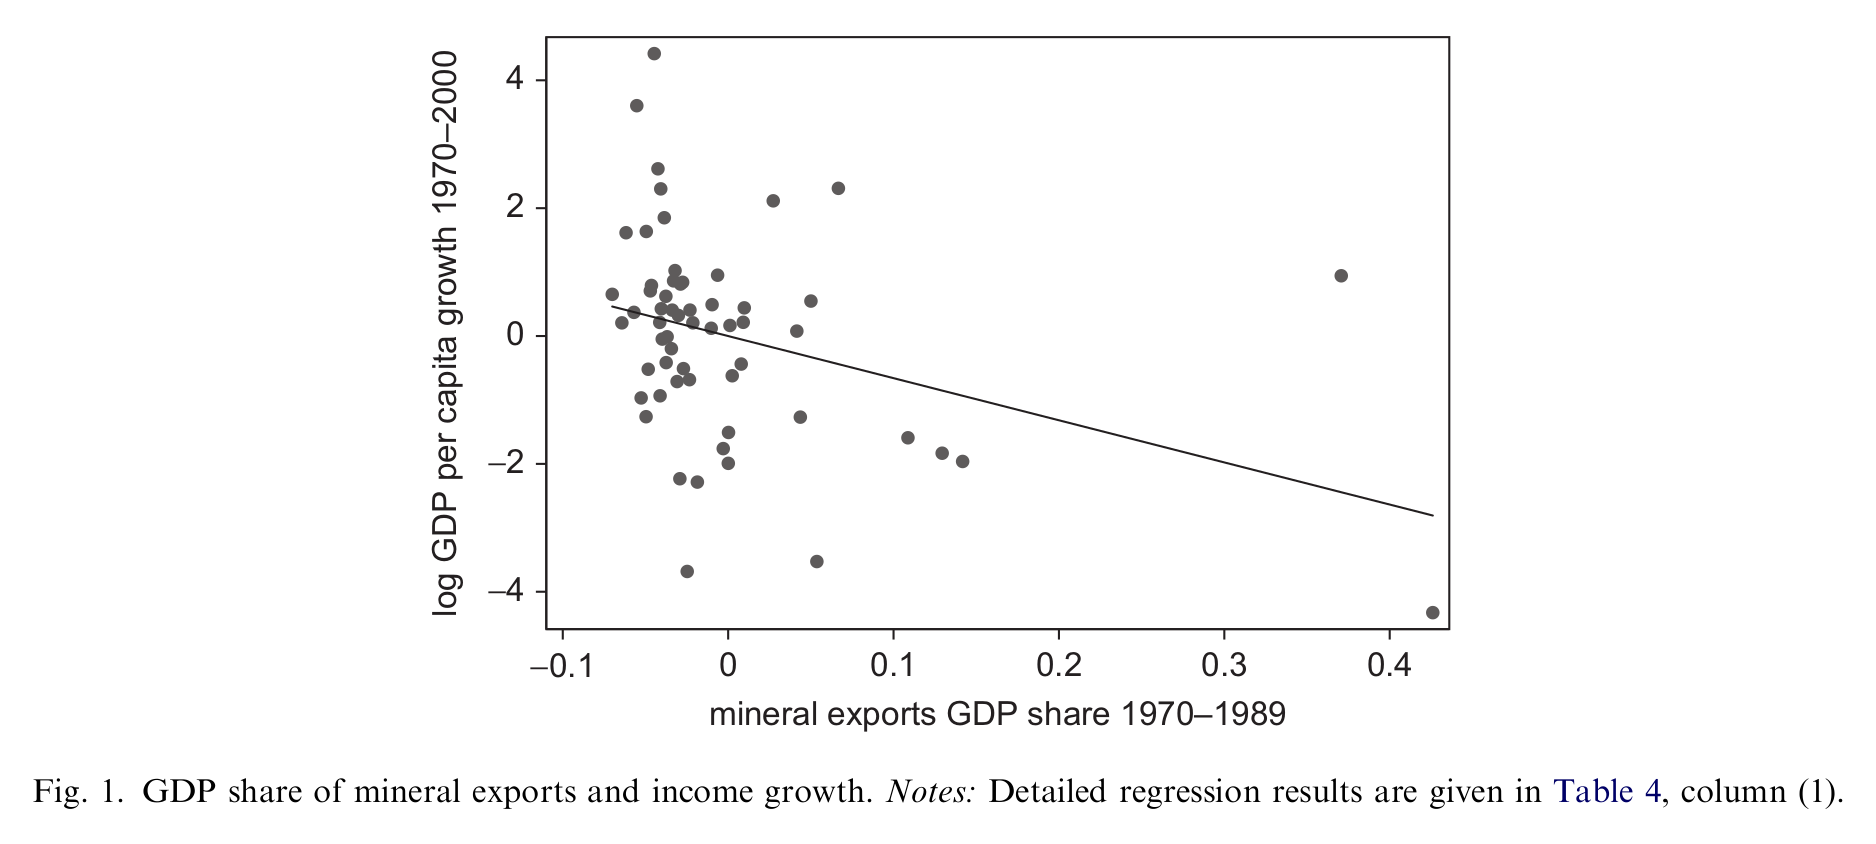
\includegraphics[scale=.7]{bulte.png}
  \end{figure}
  Brunnschweiler \& Bulte, 2008, "The resource curse revisited and revised: A tale of paradoxes and red herrings"
\end{frame}
%--------------------------------------

%--------------------------------------
\begin{frame}
 There are different explanations for how resource abundance is linked to underdevelopment
 \begin{enumerate}
  \item Rent-seeking behaviour
  \item Resource sector crowds out the non-resource sector which is more important for long-run growth due to increasing returns at the sector level
 \end{enumerate}
 \medskip
 It might not be per se abundance that leads to underdevelopment but a heavy reliance on the resources. 
\end{frame}
%--------------------------------------

%--------------------------------------
\begin{frame}
 How does trade actually promote economic growth?
 Let's consider standard Cobb-Douglas production function
 \begin{align*}
   Y_t=A_tK_t^{\alpha}L_t^{\beta}
 \end{align*}
 Re-writing to get output per worker
 \begin{align*}
   \frac{Y_t}{L_t}&=A_tK_t^{\alpha}L_t^{\beta-1} 
      \\ &= A_t \left( \frac{K_t}{L_t} \right)^{\alpha} L_t^{\alpha+\beta-1} 
 \end{align*}
\end{frame}
%--------------------------------------

%--------------------------------------
\begin{frame}
  Three ways to improve productivity and growth
  \begin{enumerate}
    \item More workers will increase productivity if 
    \begin{align*}
       \alpha+\beta>1
     \end{align*} 
     However, most growth theories assume constant returns to scale    
    \begin{align*}
      \frac{Y_t}{L_t}=A_t \left( \frac{K_t}{L_t} \right)^{\alpha}
    \end{align*}
    \item Capital deepening
    \item Technological progress
  \end{enumerate}
  \medskip
  Trade, since it fosters specialisation, leads to capital deepening and stimulates diffusion of new technologies.
\end{frame}
%--------------------------------------

%--------------------------------------
\begin{frame}
  \begin{figure}
    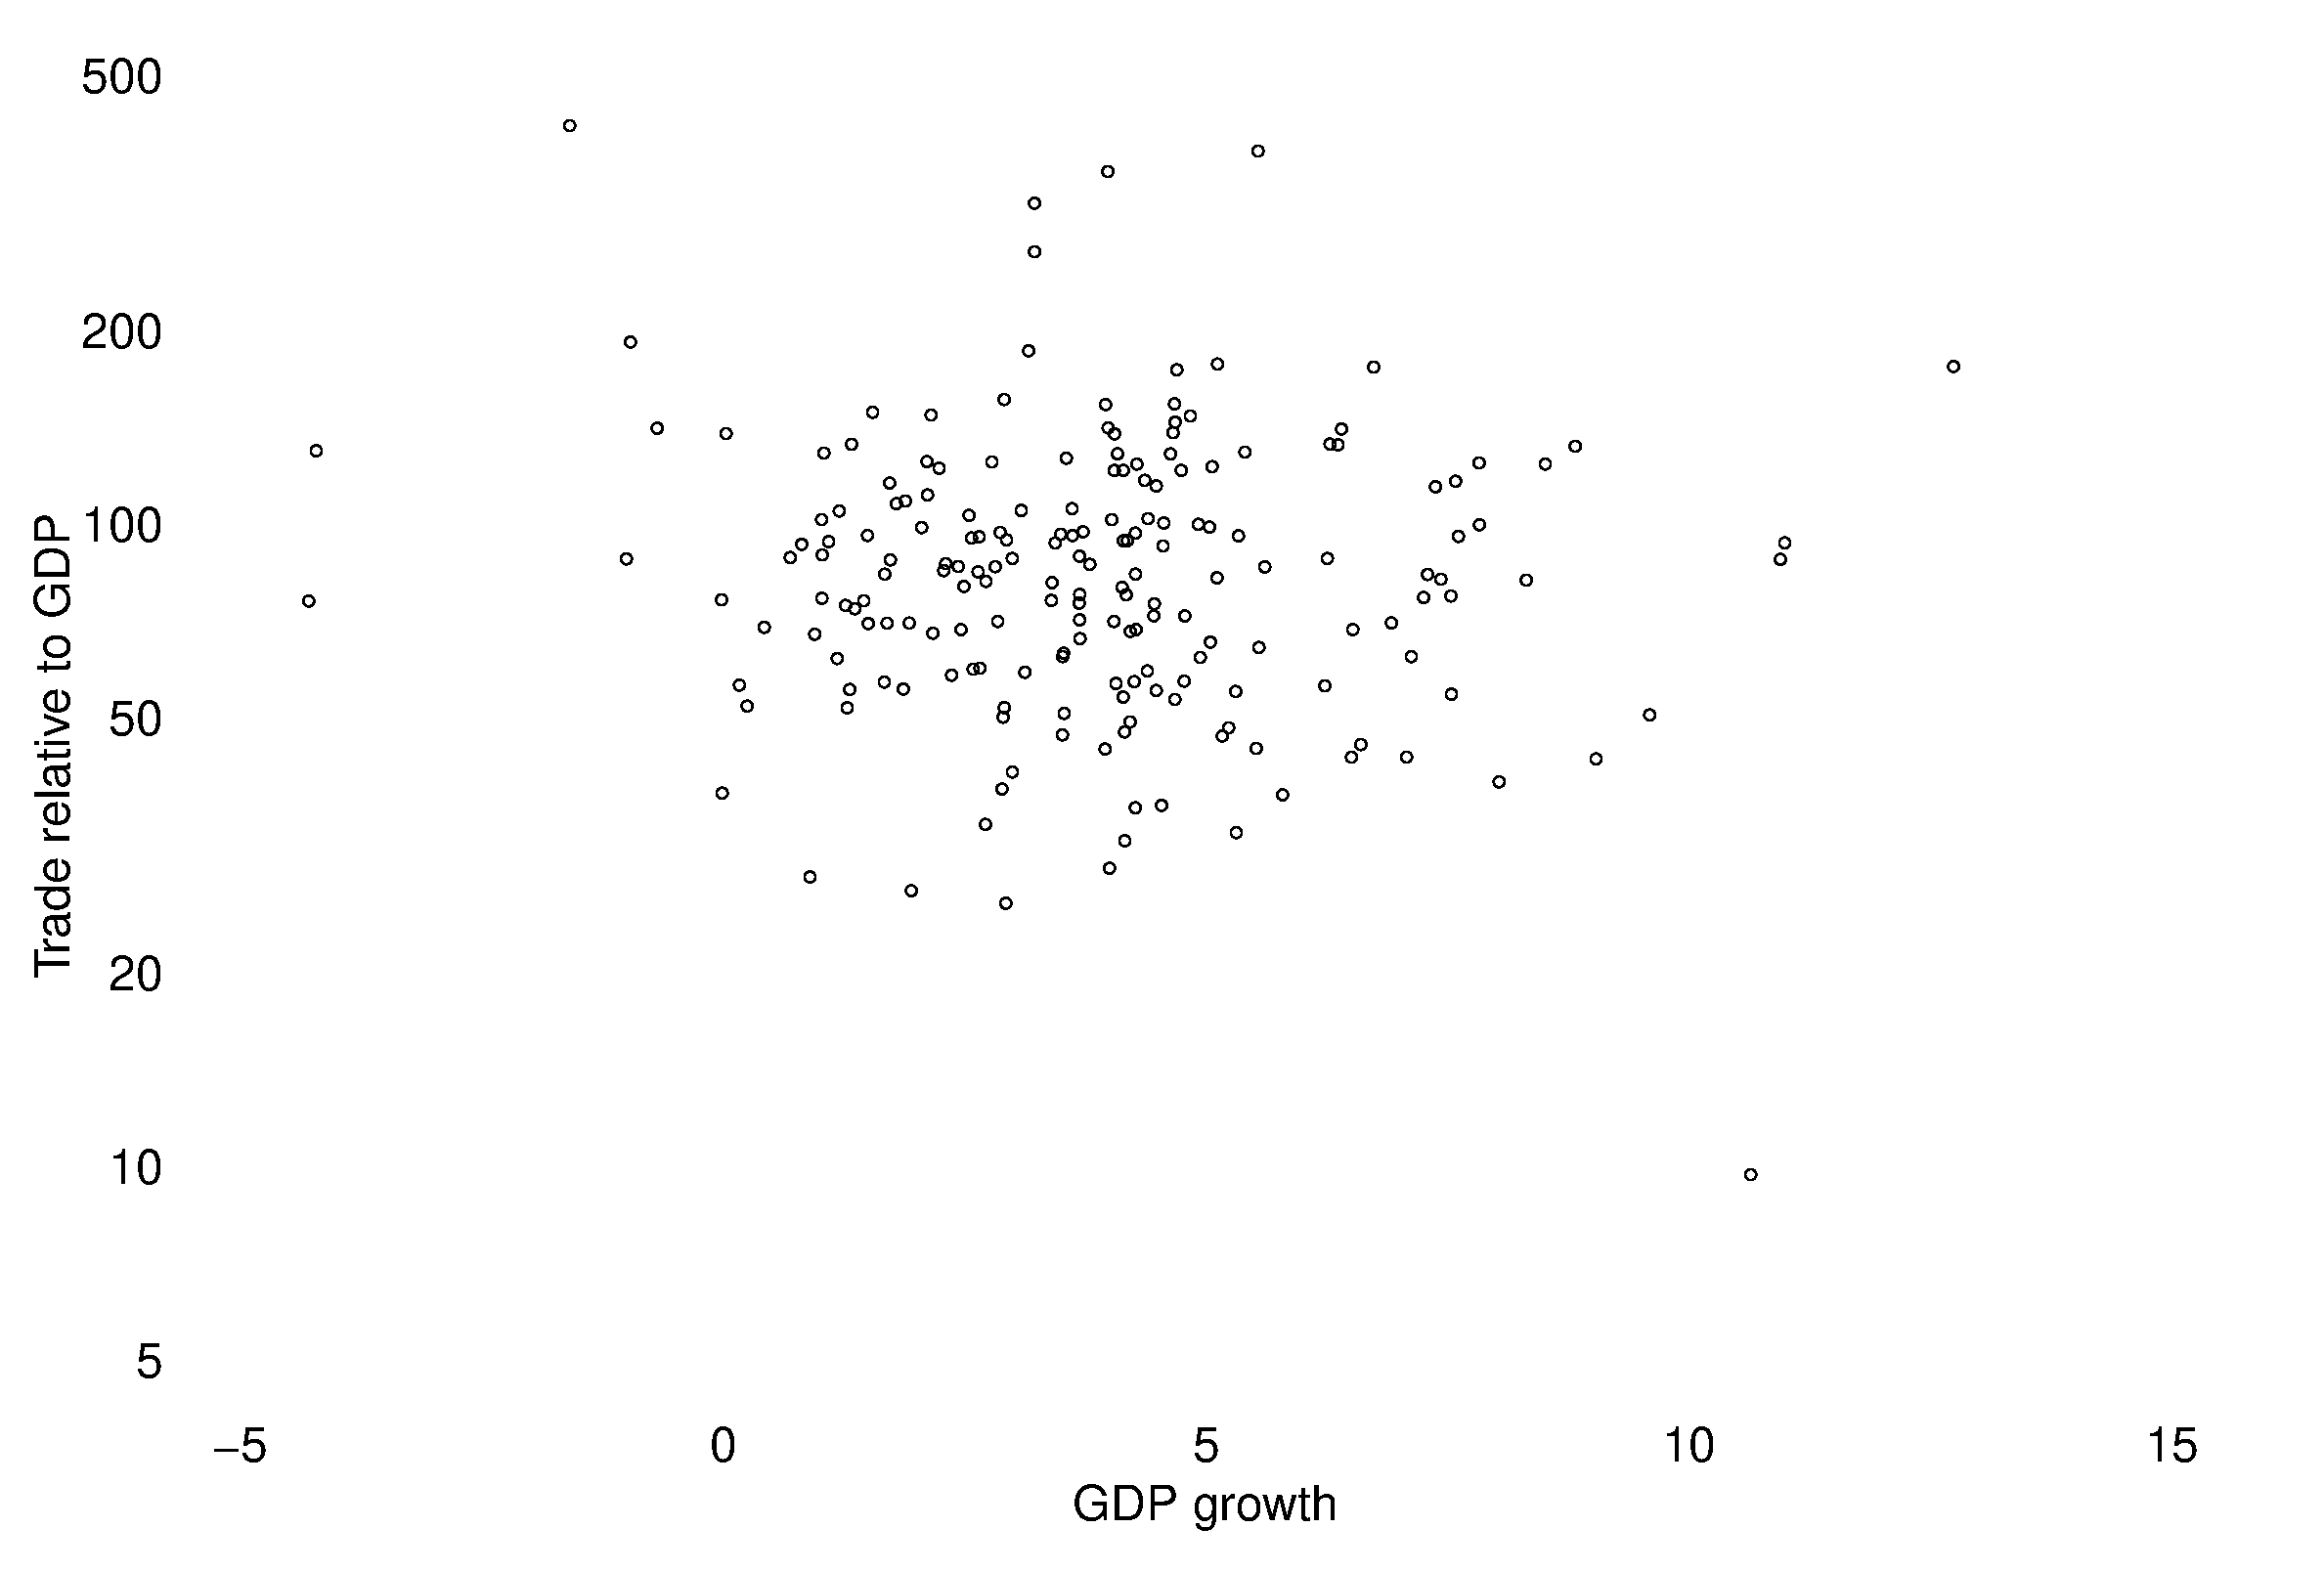
\includegraphics[scale=.3]{trade_gdp.eps}
  \end{figure}
\end{frame}
%--------------------------------------

%--------------------------------------
\begin{frame}
There are three basic trade strategies for development
 \begin{enumerate}
   \item Import-substituting industrialisation
   \item Export-oriented industrialisation
   \item Trade liberalisation 
 \end{enumerate}
\end{frame}
%--------------------------------------

%--------------------------------------
\begin{frame}
 Import-substituting industrialisation (ISI) is a development strategy that aims to reduce foreign dependency by 
 \begin{itemize}
   \item Replacing imports with domestic production
   \item Encouraging domestic production
 \end{itemize}
 \medskip
 There are two stages
 \begin{enumerate}
   \item Use tariffs and quotas to reduce imports, which will increase domestic prices and therefore production
   \item Industrial diversification focusing mainly on manufactured goods.    
 \end{enumerate}
 \medskip
 ISI strategy partially driven by Prebisch-Singer hypothesis
\end{frame}
%--------------------------------------

%--------------------------------------
\begin{frame}
 ISI was adapted by many low- and middle-income countries before the 1980's.
 \begin{itemize}
   \item Predominantly in what is called the Global South
   \item Particularly popular in Central and South America during the 1950-60's
 \end{itemize}
 \medskip
 This was in a time when European colonialism came to an end which led to a belief that Western countries exploit others through international financial markets and trade. 
\end{frame}
%--------------------------------------

%--------------------------------------
\begin{frame}
 An import justification for ISI is the \textbf{infant industry argument}. 
 \begin{itemize}
   \item A country could have a potential comparative advantage in certain industries
   \item But no economies of scale to compete with foreign competitors
   \item Therefore the government should support these industries until they are strong enough
 \end{itemize}
 \medskip
 This is a valid argument in the presence of imperfect capital markets and if there is learning-by-doing
\end{frame}
%--------------------------------------

%--------------------------------------
\begin{frame}
  There are a number of counterarguments to be made regarding the protection of infant industries
  \begin{enumerate}
    \item May be wasteful to support industries that will have a future comparative advantage
    \item With protection industries might never become competitive
    \item No need for government protection in absence of market failure
  \end{enumerate}
  \medskip
  In practice policy result often corruption and monopolies.
\end{frame}
%--------------------------------------

%--------------------------------------
\begin{frame}
 One important point is that the presence of market failure could prevent the industry from becoming competitive. 
 Market failure could arise due to
 \begin{enumerate}
   \item Imperfect capital markets
   \begin{itemize}
     \item When there are imperfect capital markets poorly working financial laws and markets will restrict borrowing of new industries and hamper economic growth
     \item Creating tariffs would be a second-best option to increase profits of new industry
   \end{itemize}
   \medskip
   \item Appropriability problem
   \begin{itemize}
     \item Firms might not be able to appropriate benefits from investment in new industries
     \item Knowledge created by industry might not be appropriable due to lack of property rights
     \item If establishing system of property rights is not feasible, tariffs are a second best policy to encourage growth
   \end{itemize}
 \end{enumerate}
\end{frame}
%--------------------------------------

%--------------------------------------
\begin{frame}
 Can a developing country protect its economy using a tariff?
 One would argue that a developing country has the same advantages of free trade as any other country
 \begin{itemize}
   \item Can exploit comparative advantage to increase efficiency
   \item Can promote growth through trade
 \end{itemize}
 \medskip
 However, a problem is that developing countries are lagging and therefore can't compete on the international market
 \begin{itemize}
   \item Note that all developed countries have used tariffs in the past
 \end{itemize}
\end{frame}
%--------------------------------------


%--------------------------------------
\begin{frame}
 In the end ISI didn't really work out and lead to a disconnect with the developed world, reducing exports and some extreme measures of protection
 \begin{itemize}
   \item Import to GDP ratio equaled 3\% in India in the early 1970's\footnote{Excluding oil}
   \item Some effective tariff rates: Mexico, 26\%; Philippines, 61\%; Brazil, 113\%; Chile, 182\%; Pakistan, 271\%
 \end{itemize}
\end{frame}
%--------------------------------------

%--------------------------------------
\begin{frame}
 ISI lost track in the 1980's due to poor performance in the import-substitution industries and the fact that countries that adapted export-led growth policies did much better.
 There are a number of explanations for the failure of ISI which include
 \begin{enumerate}
   \item Production on too small scale
   \item Production distorted through rent-seeking
   \item Increased costs of doing business due to bureaucracy
 \end{enumerate}
\end{frame}
%--------------------------------------

%--------------------------------------
\begin{frame}
 ISI was popular in Central and South America where during the 1950-60s it helped develop manufacturing sectors.
 However, during the 1970s further ISI possibilities disappeared
 \begin{itemize}
   \item Industrial growth slowed down and urban jobs became scarce
   \item Income distribution didn't improve either
 \end{itemize}
 \medskip
 Due to high prices export possibilities were limited and ISI was abandoned in the 1980's.
\end{frame}
%--------------------------------------


%--------------------------------------
\begin{frame}
  Export-oriented industrialisation used policies to expand the country's exports
  \begin{itemize}
    \item Agricultural commodities and raw materials
    \item Manufactured goods
  \end{itemize}
\end{frame}
%--------------------------------------

%--------------------------------------
\begin{frame}
  Given that economies of most developing countries are dominated by the primary sector it would make sense to focus on exports
  \begin{itemize}
    \item Domestic demand is too low to promote growth
  \end{itemize}
  \medskip
  There are however some foreign demand factors that work against this strategy
  \begin{itemize}
    \item Prebisch-Singer hypothesis
    \item Low population growth in developed countries
    \item Synthetic substitutes
    \item Protection in developed countries
  \end{itemize}
\end{frame}
%--------------------------------------

%--------------------------------------
\begin{frame}
 Implemented policies in export-oriented industrialisation often focused on particular industries.
 \begin{itemize}
   \item Making use of their comparative advantage, these countries experienced rapid economic growth in export sectors as well as in general   
  \end{itemize}
  \medskip 
 These countries generated high volumes of export and import relative to total production.
 \begin{itemize}
   \item Although they are open economies they still have high restrictions on some forms of trade.
 \end{itemize}
\end{frame}
%--------------------------------------

%--------------------------------------
\begin{frame}
 Countries focusing on export-led growth implemented a number of different policies to achieve their goals.
 \begin{itemize}
   \item This included subsidised loans, and research and development
 \end{itemize}
 \medskip
 But it is hard to establish the effect of the implemented policies and there is little evidence to suggest that these countries experienced higher growth rates in the targeted industries. 
 There is some evidence that the policies actually failed.
 \begin{itemize}
   \item For instance the South Korean auto industry in the 1970s
   \item Was abandoned as it was too expensive and did not lead to the desired growth
 \end{itemize}
\end{frame}
%--------------------------------------

%--------------------------------------
\begin{frame}
  Some countries did well using this approach such as the four tigers
  \begin{enumerate}
    \item Hong Kong
    \item Singapore
    \item South Korea
    \item Taiwan
  \end{enumerate}
  \medskip
  A number of other countries which adopted this strategy later also did well
  \begin{enumerate}
    \item Thailand
    \item Indonesia
    \item Philippines
  \end{enumerate}
  \medskip
  Untill the 1997 financial crisis.
\end{frame}
%--------------------------------------

%--------------------------------------
\begin{frame}
  \begin{figure}
    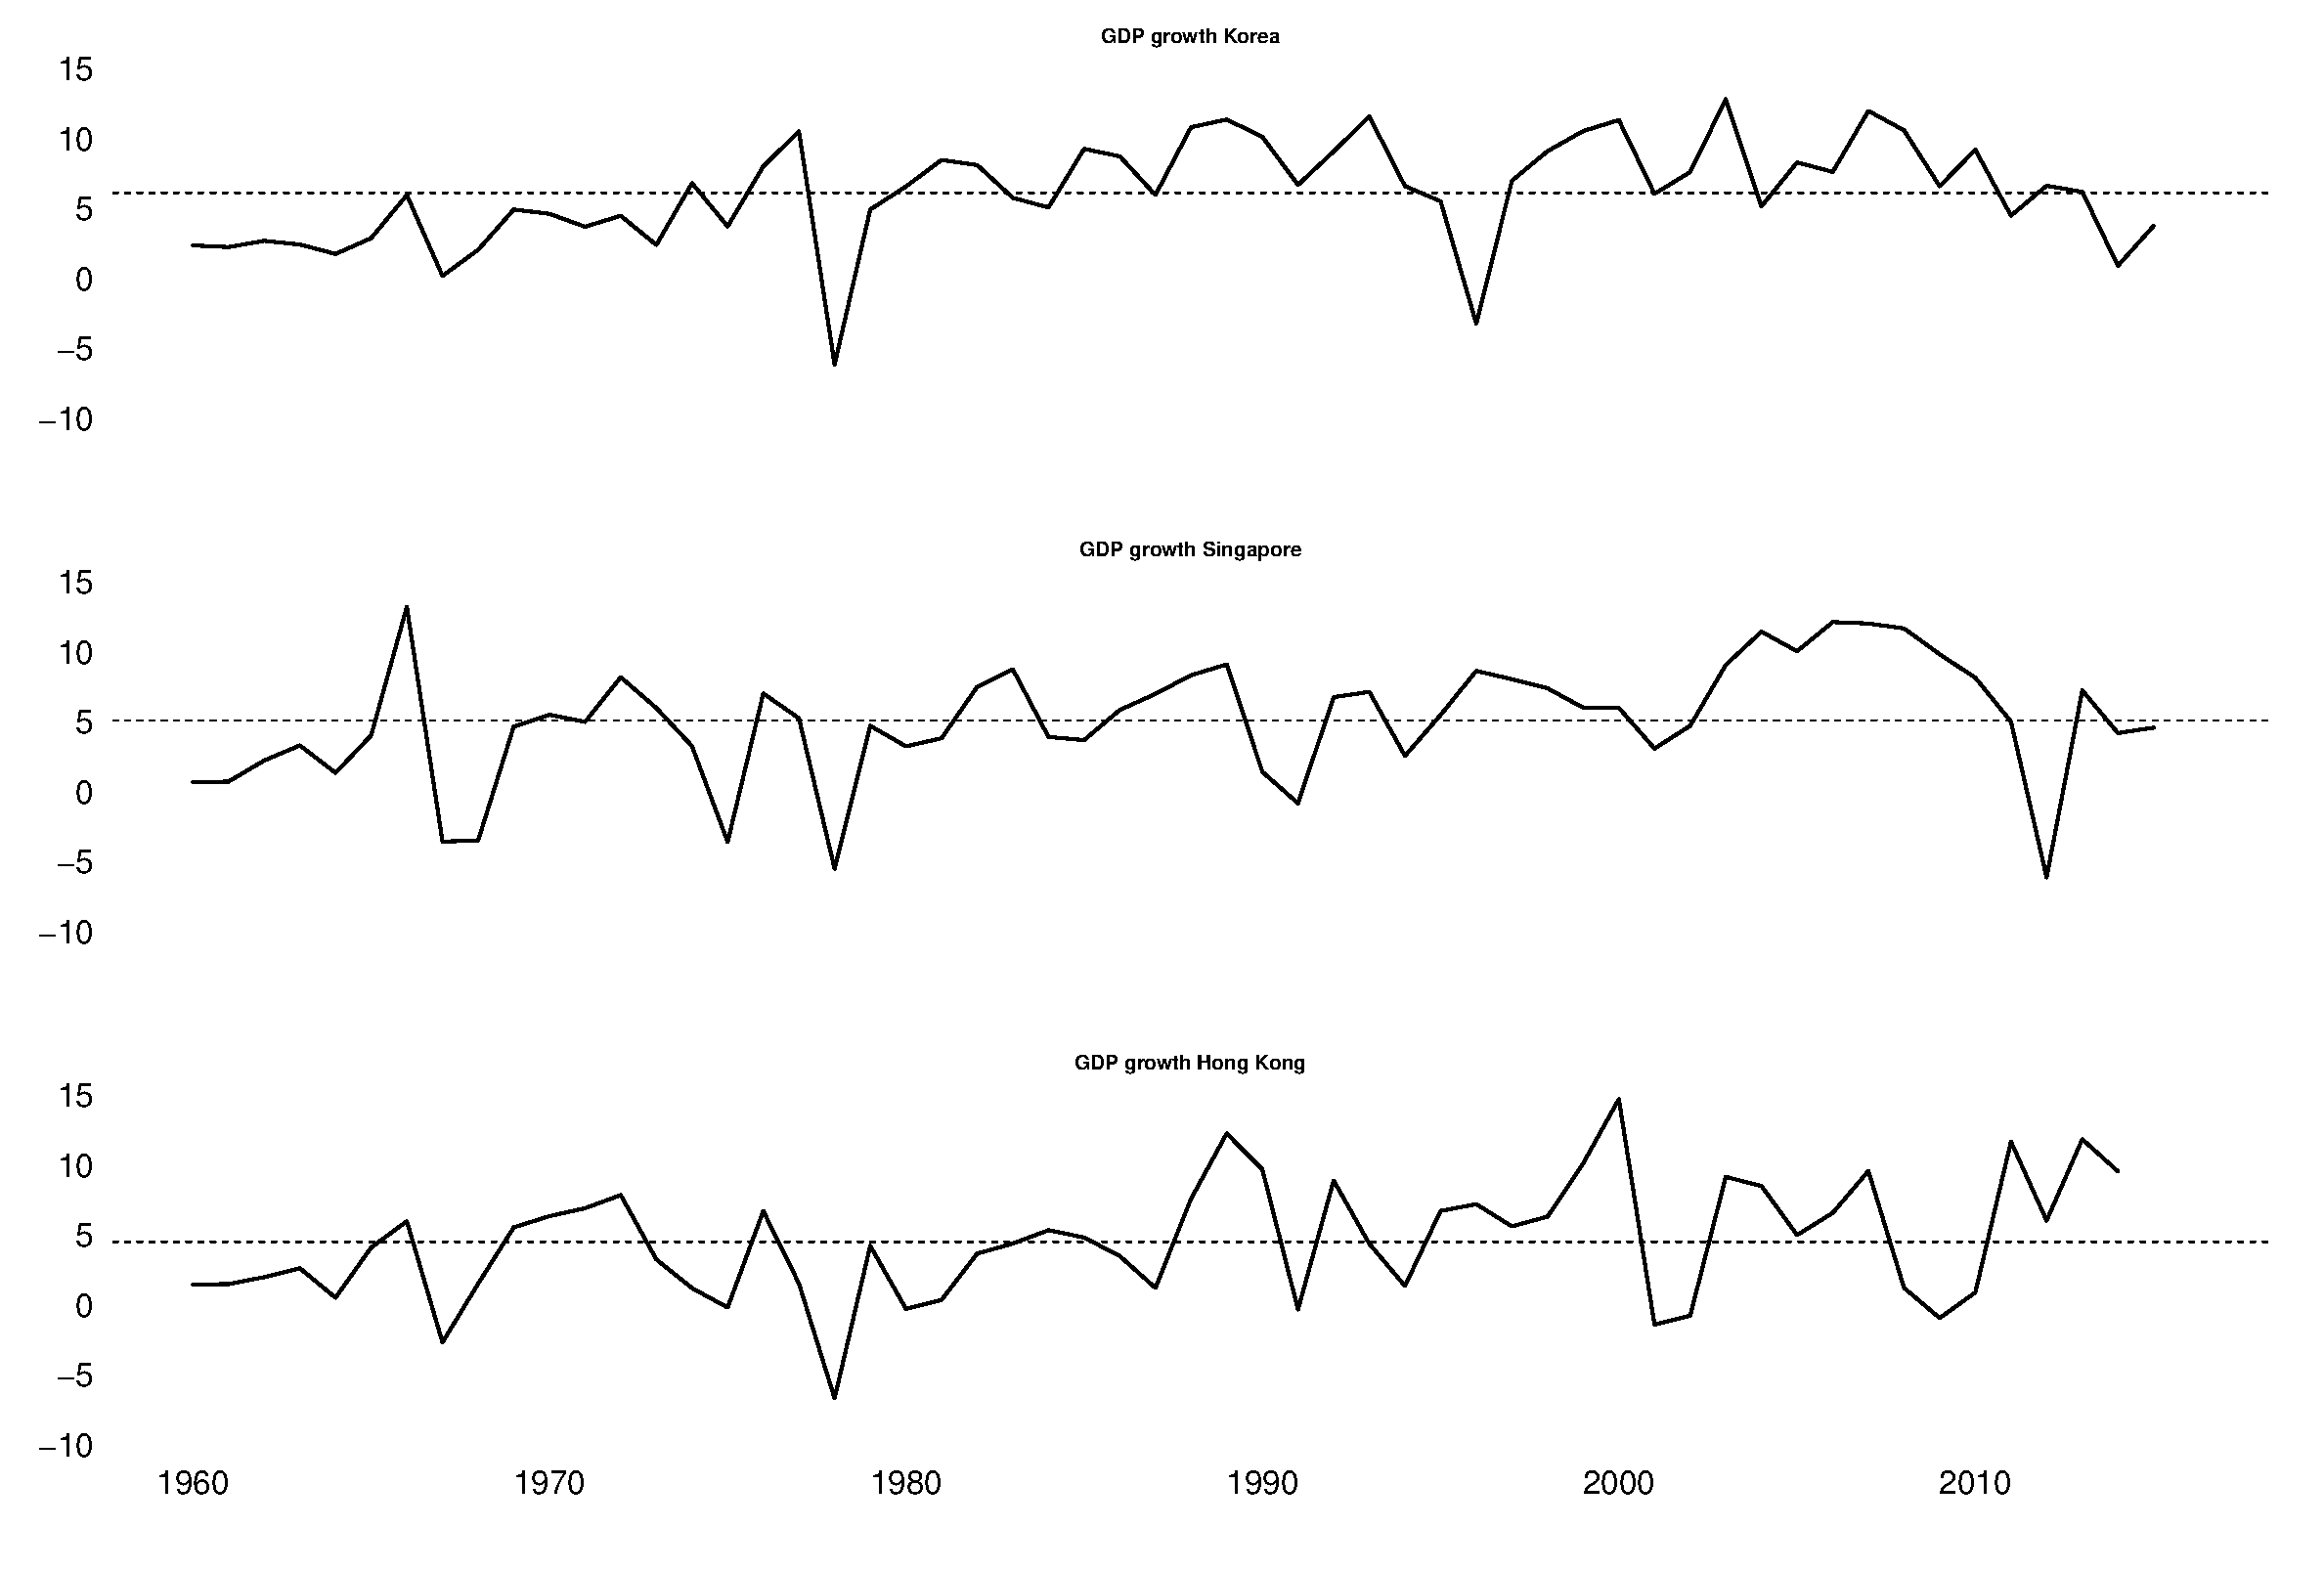
\includegraphics[scale=.3]{asian_tigers.eps}
  \end{figure}
\end{frame}
%--------------------------------------

%--------------------------------------
\begin{frame}
  \begin{figure}
    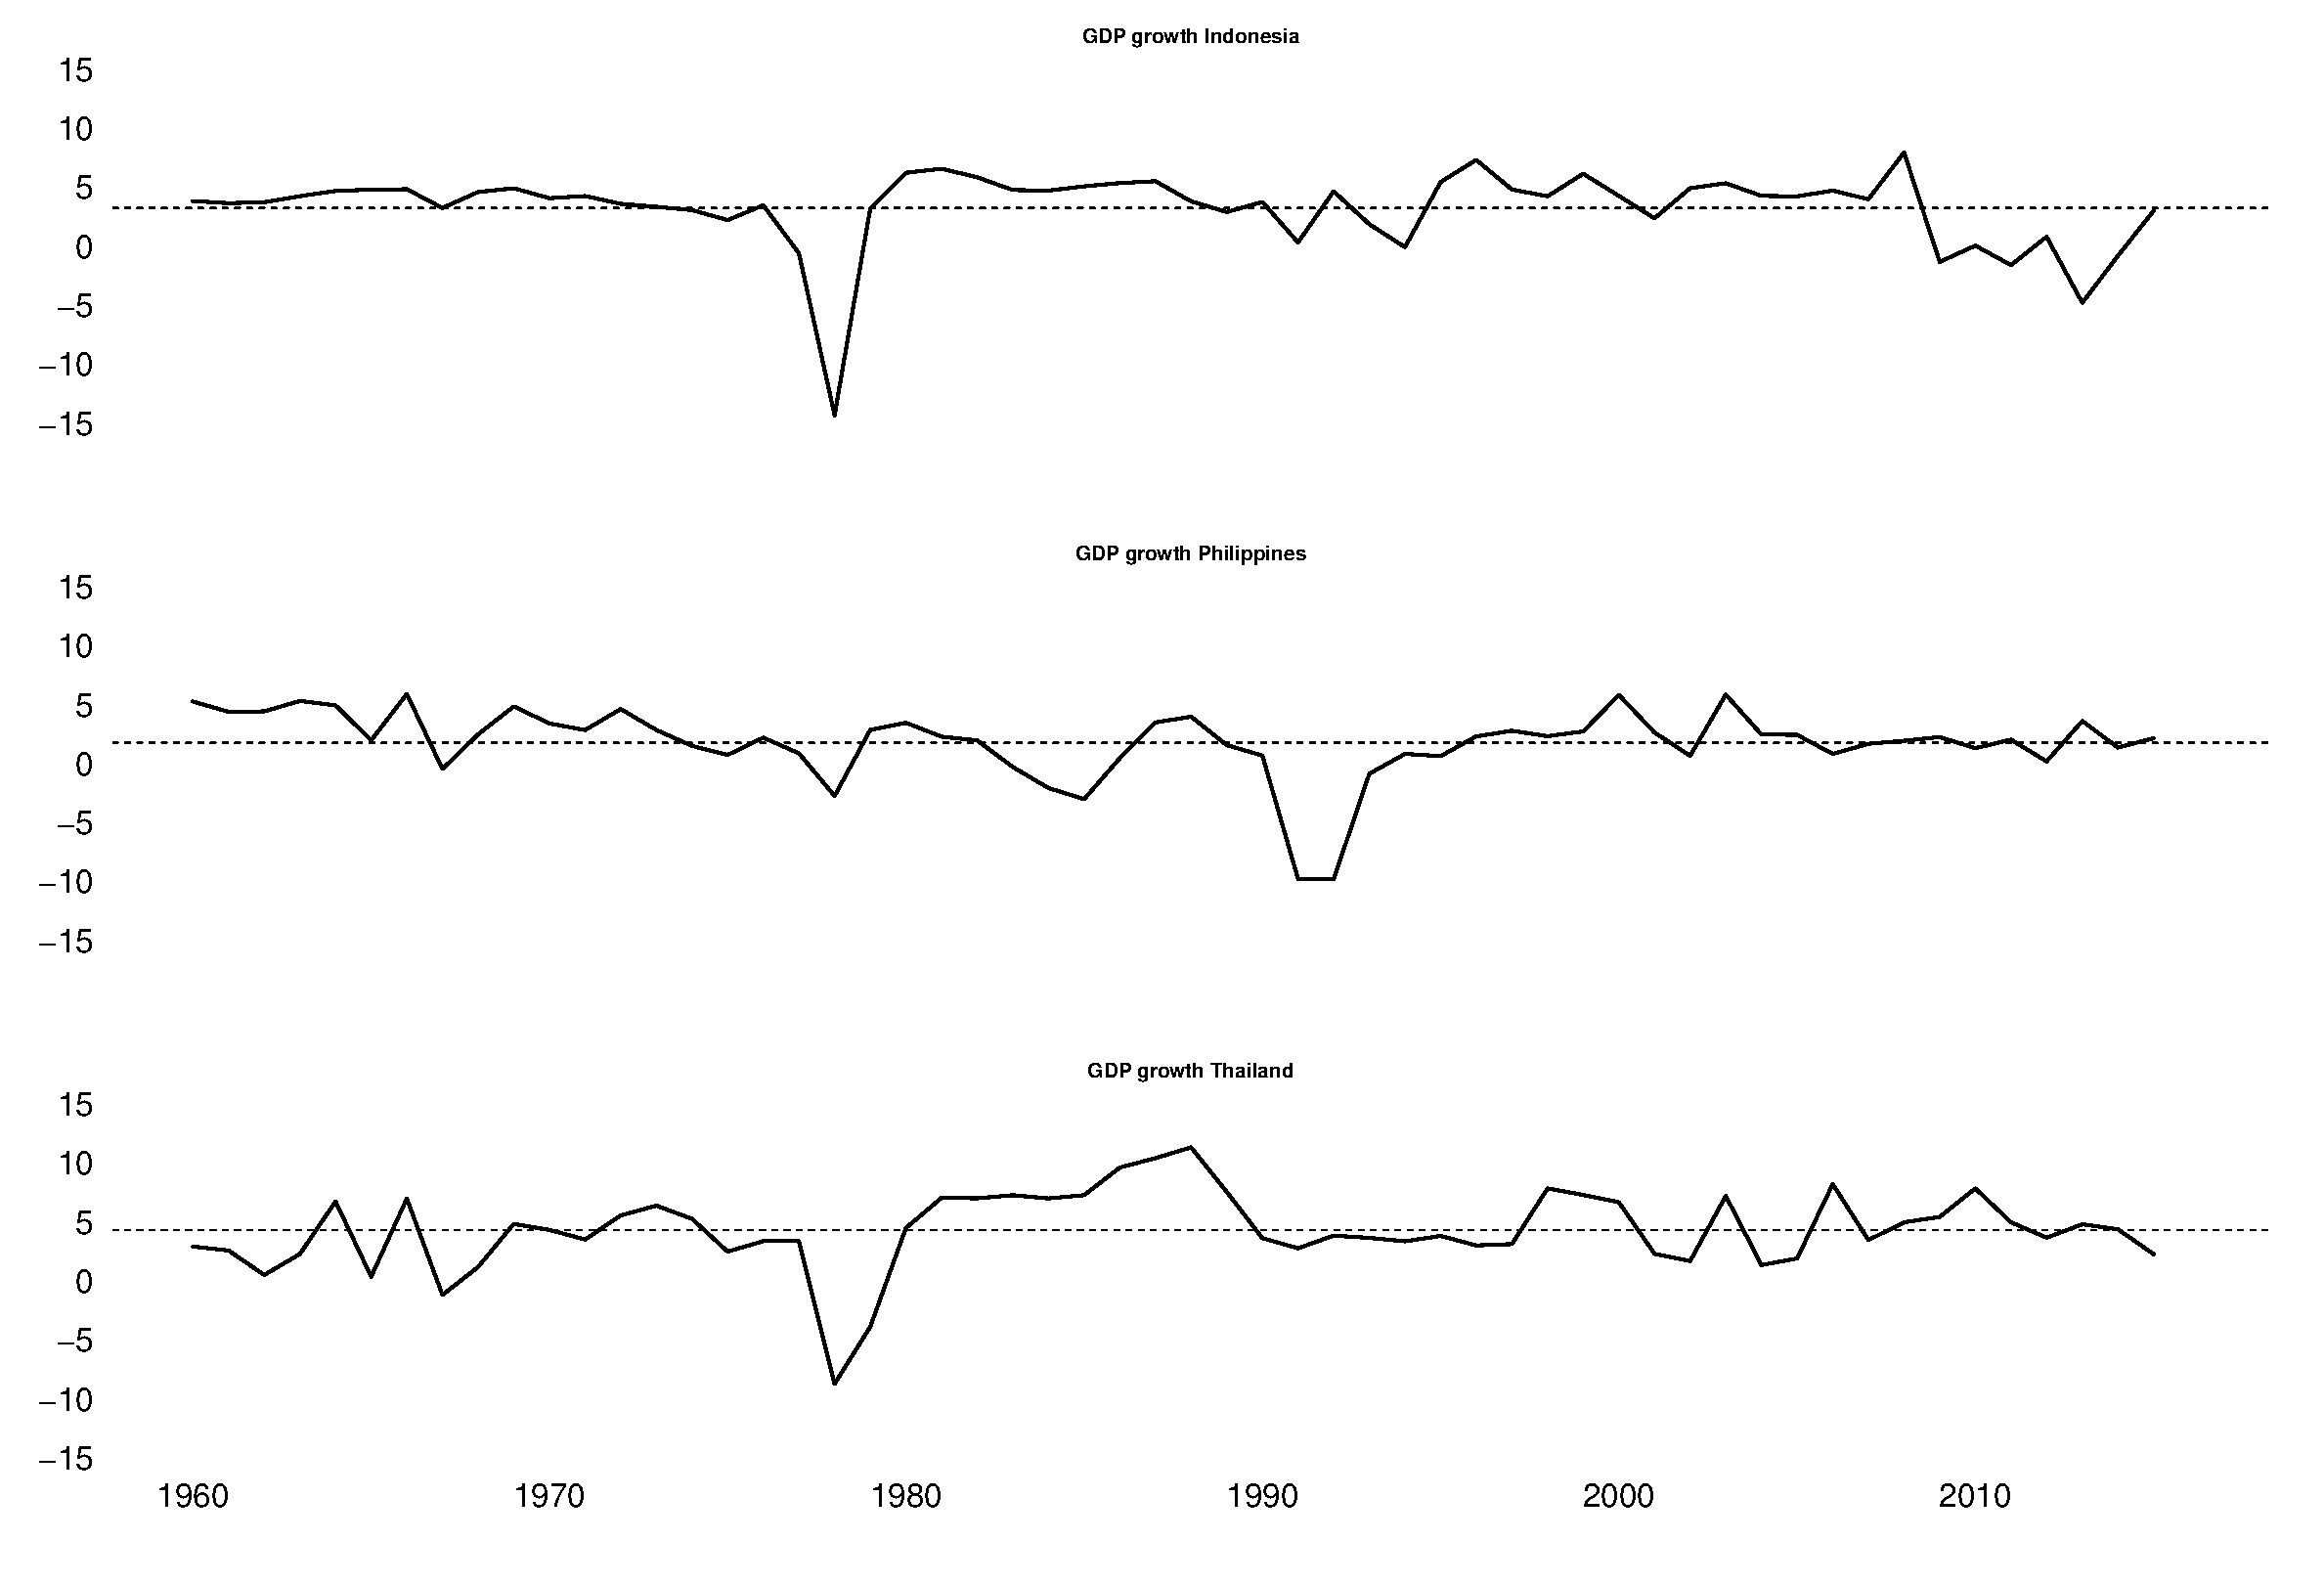
\includegraphics[scale=.3]{asian_tigers2.eps}
  \end{figure}
\end{frame}
%--------------------------------------



%--------------------------------------
\begin{frame}
  It is unclear whether the exports caused growth or just happens to be correlated.
  \begin{enumerate}
    \item High savings and investment rates lead to high general growth rates and growth in export sectors
    \item There was a rapid growth in education levels which is important for a productive labour force
  \end{enumerate}
  \medskip
  What is clear is that countries adopting ISI such as Brazil and Mexico did not experience the same growth spur as countries such as South Korea did.
\end{frame}
%--------------------------------------

%--------------------------------------
\begin{frame}
 Just a note: For a large country, when economic growth is biased towards the export good there is the risk of something called \textbf{immiserising growth}
 \begin{itemize}
   \item Export supply affects export prices, which affects terms-of-trade
 \end{itemize}
 \medskip
 The ToT effect might outweigh the positive effect of economic growth
 \begin{itemize}
   \item This is an extreme case scenario
 \end{itemize}
\end{frame}
%--------------------------------------

%--------------------------------------
\begin{frame}
 Trade policies such as ISI and export-oriented growth were aimed at promoting economic growth, but experiences have been mixed.
 Since 1980s most developing countries have started in a process of trade liberalisation.
 \begin{itemize}
   \item Increase in average trade-to-GDP ratio 
   \item Tariff reduction of about 22 points
 \end{itemize}
 \medskip
 There does seem to be some convergence between post-1980 globalisers and industrialised countries
 \begin{itemize}
   \item More protectionist countries are falling behind
 \end{itemize} 
\end{frame}
%--------------------------------------

%--------------------------------------
\begin{frame}
  \begin{figure}
    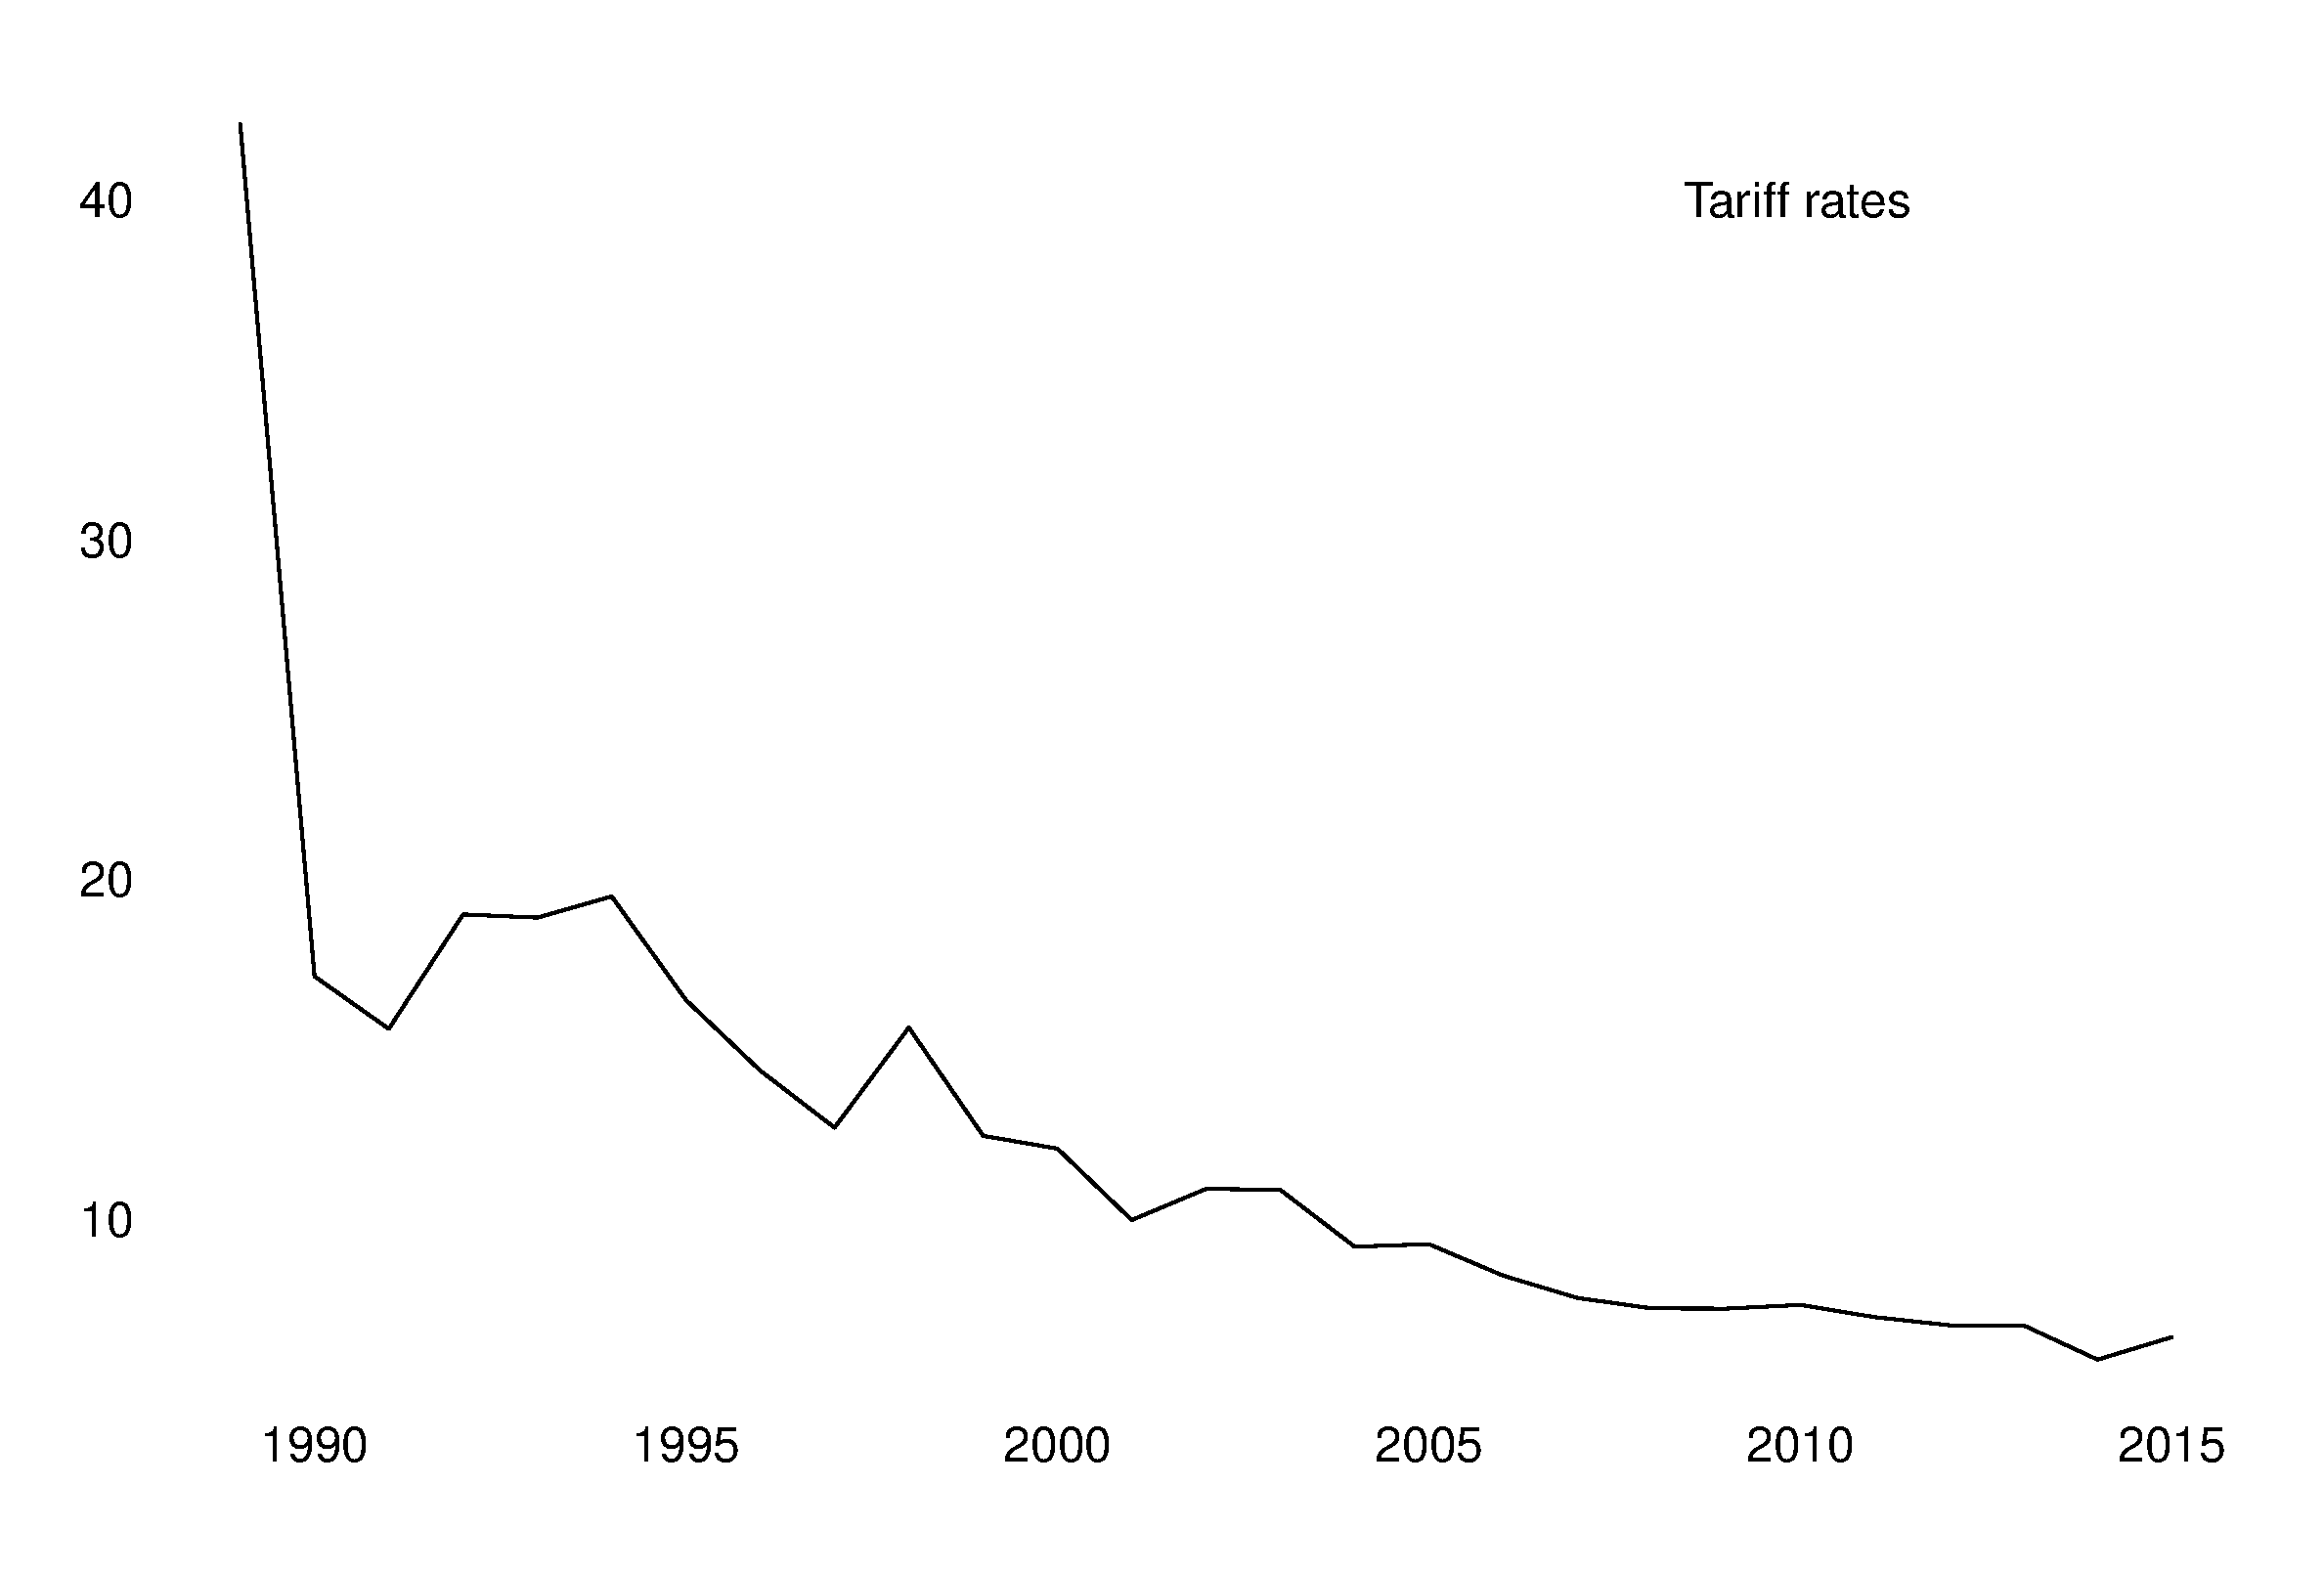
\includegraphics[scale=.3]{tariffs.eps}
  \end{figure}
\end{frame}
%--------------------------------------

%--------------------------------------
\begin{frame}
  \begin{figure}
    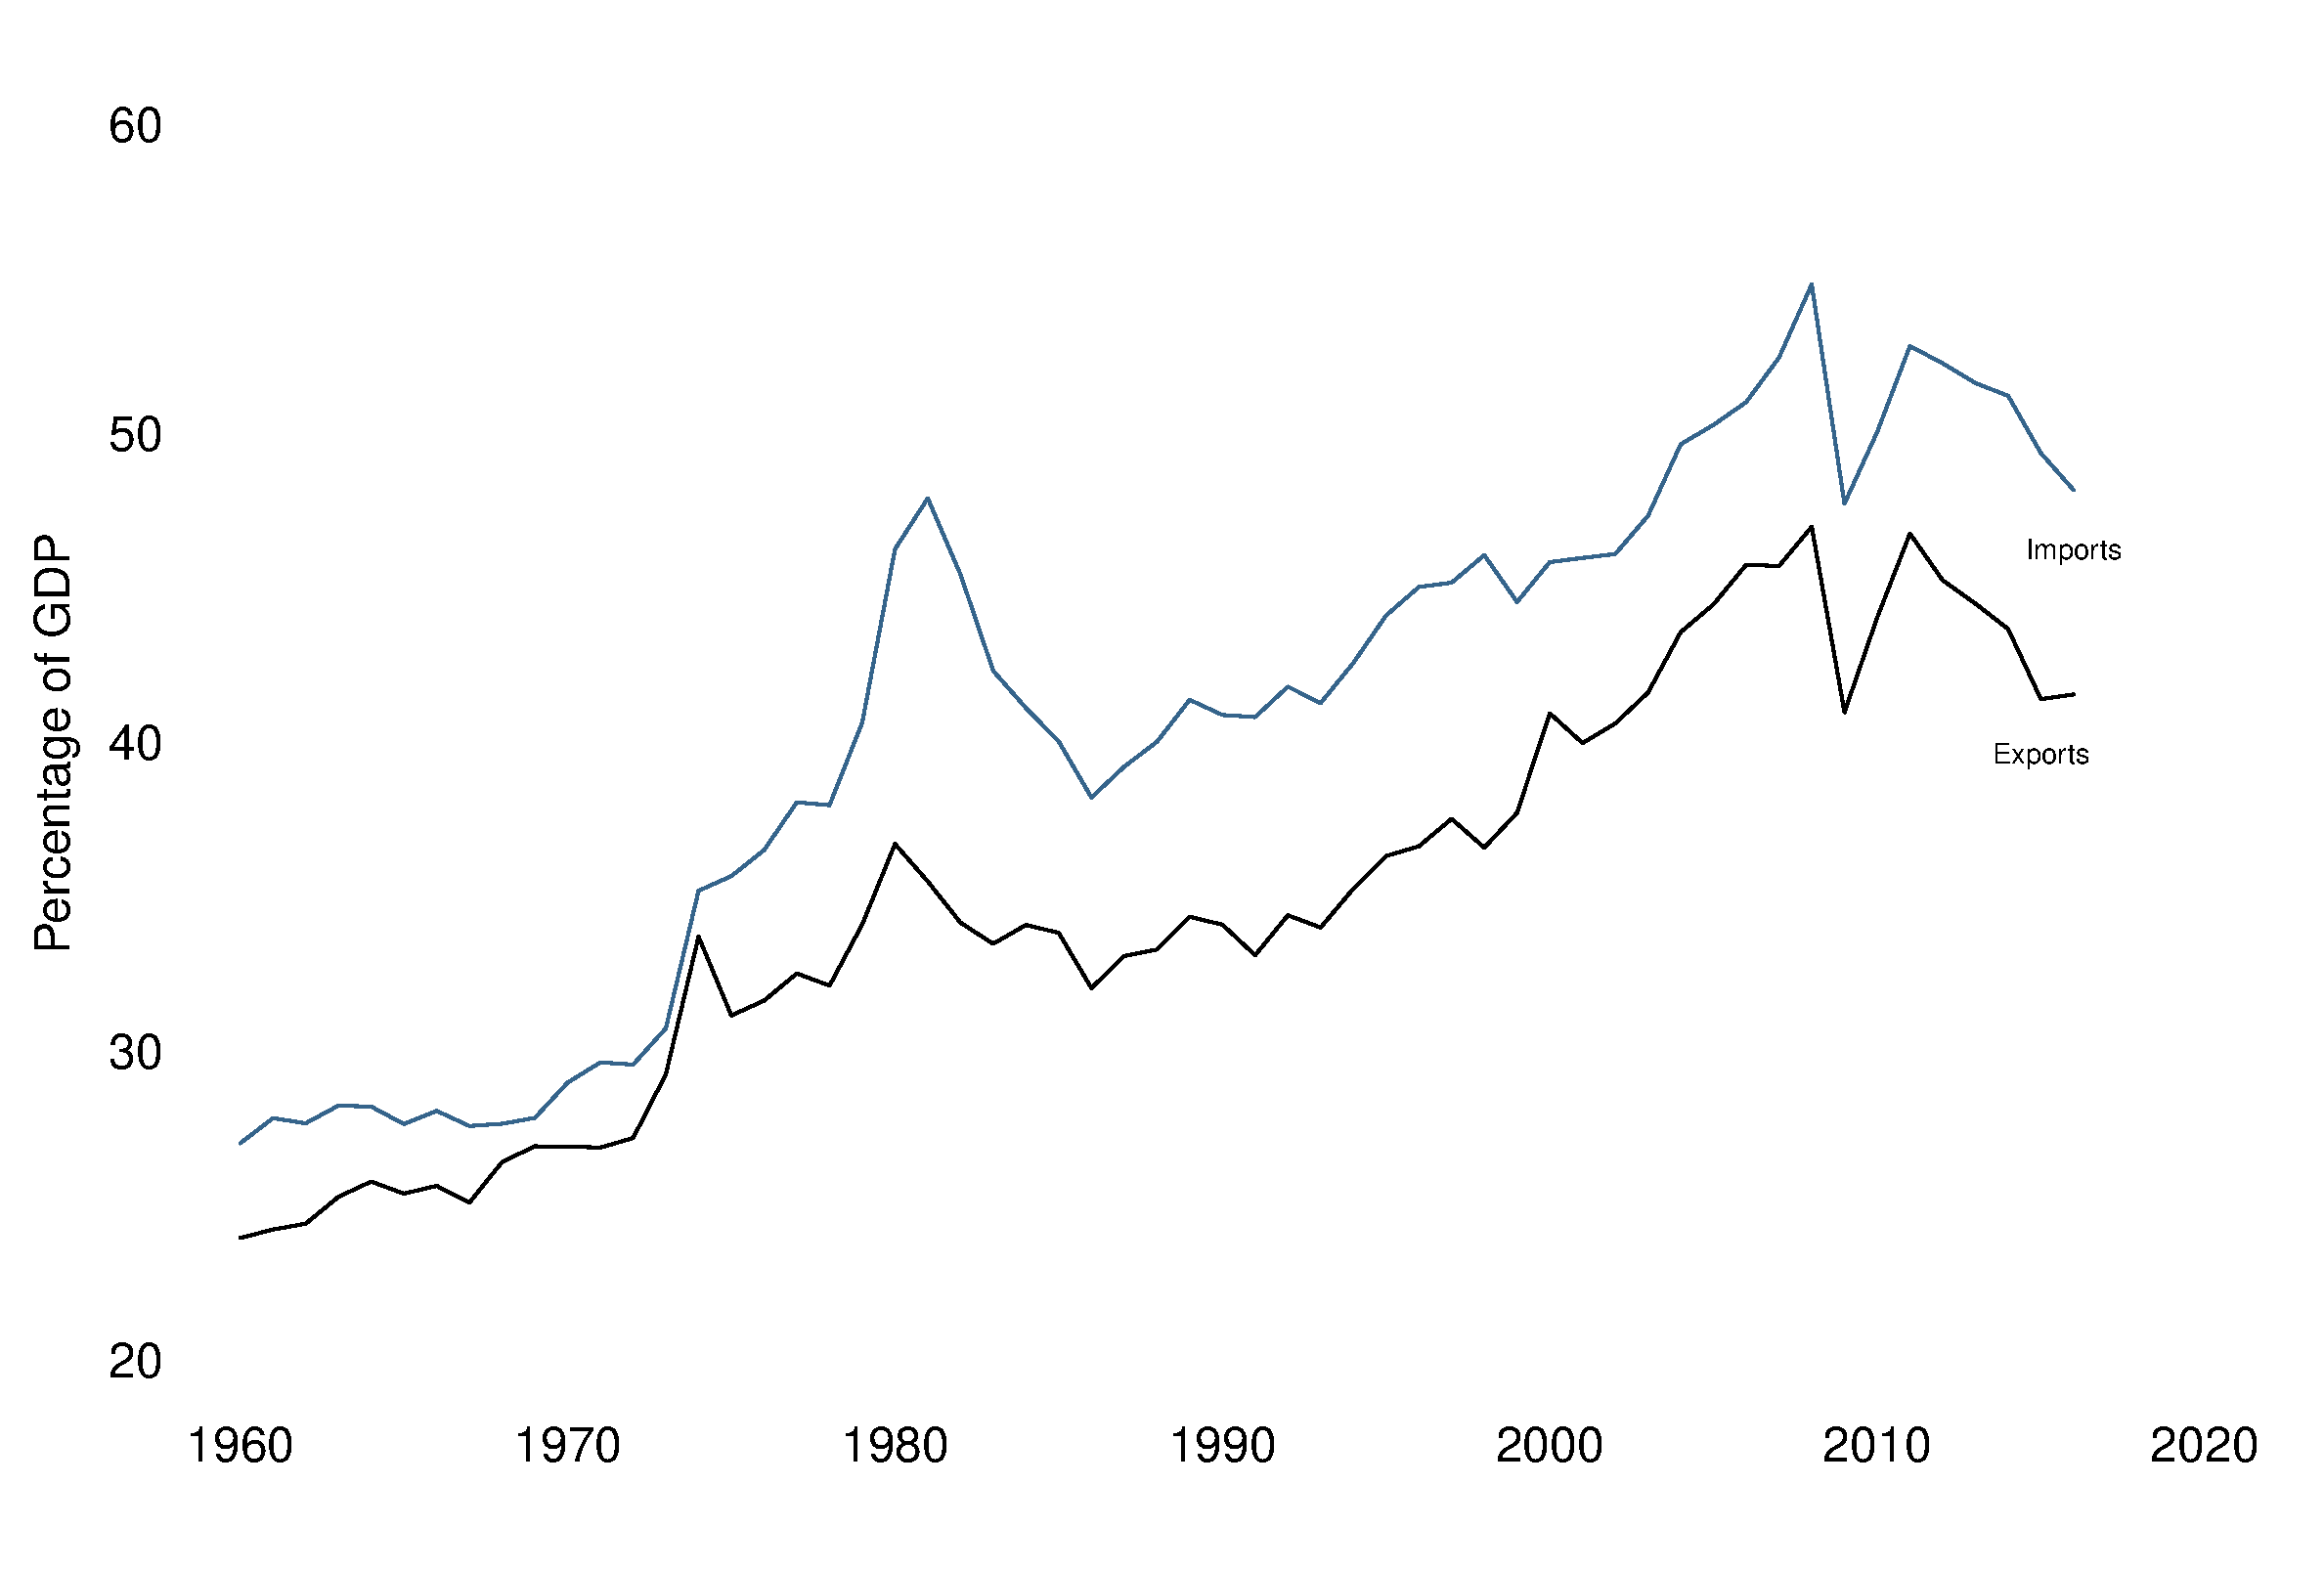
\includegraphics[scale=.3]{trade_flows.eps}
  \end{figure}
\end{frame}
%--------------------------------------

%--------------------------------------
\begin{frame}
  \begin{figure}
    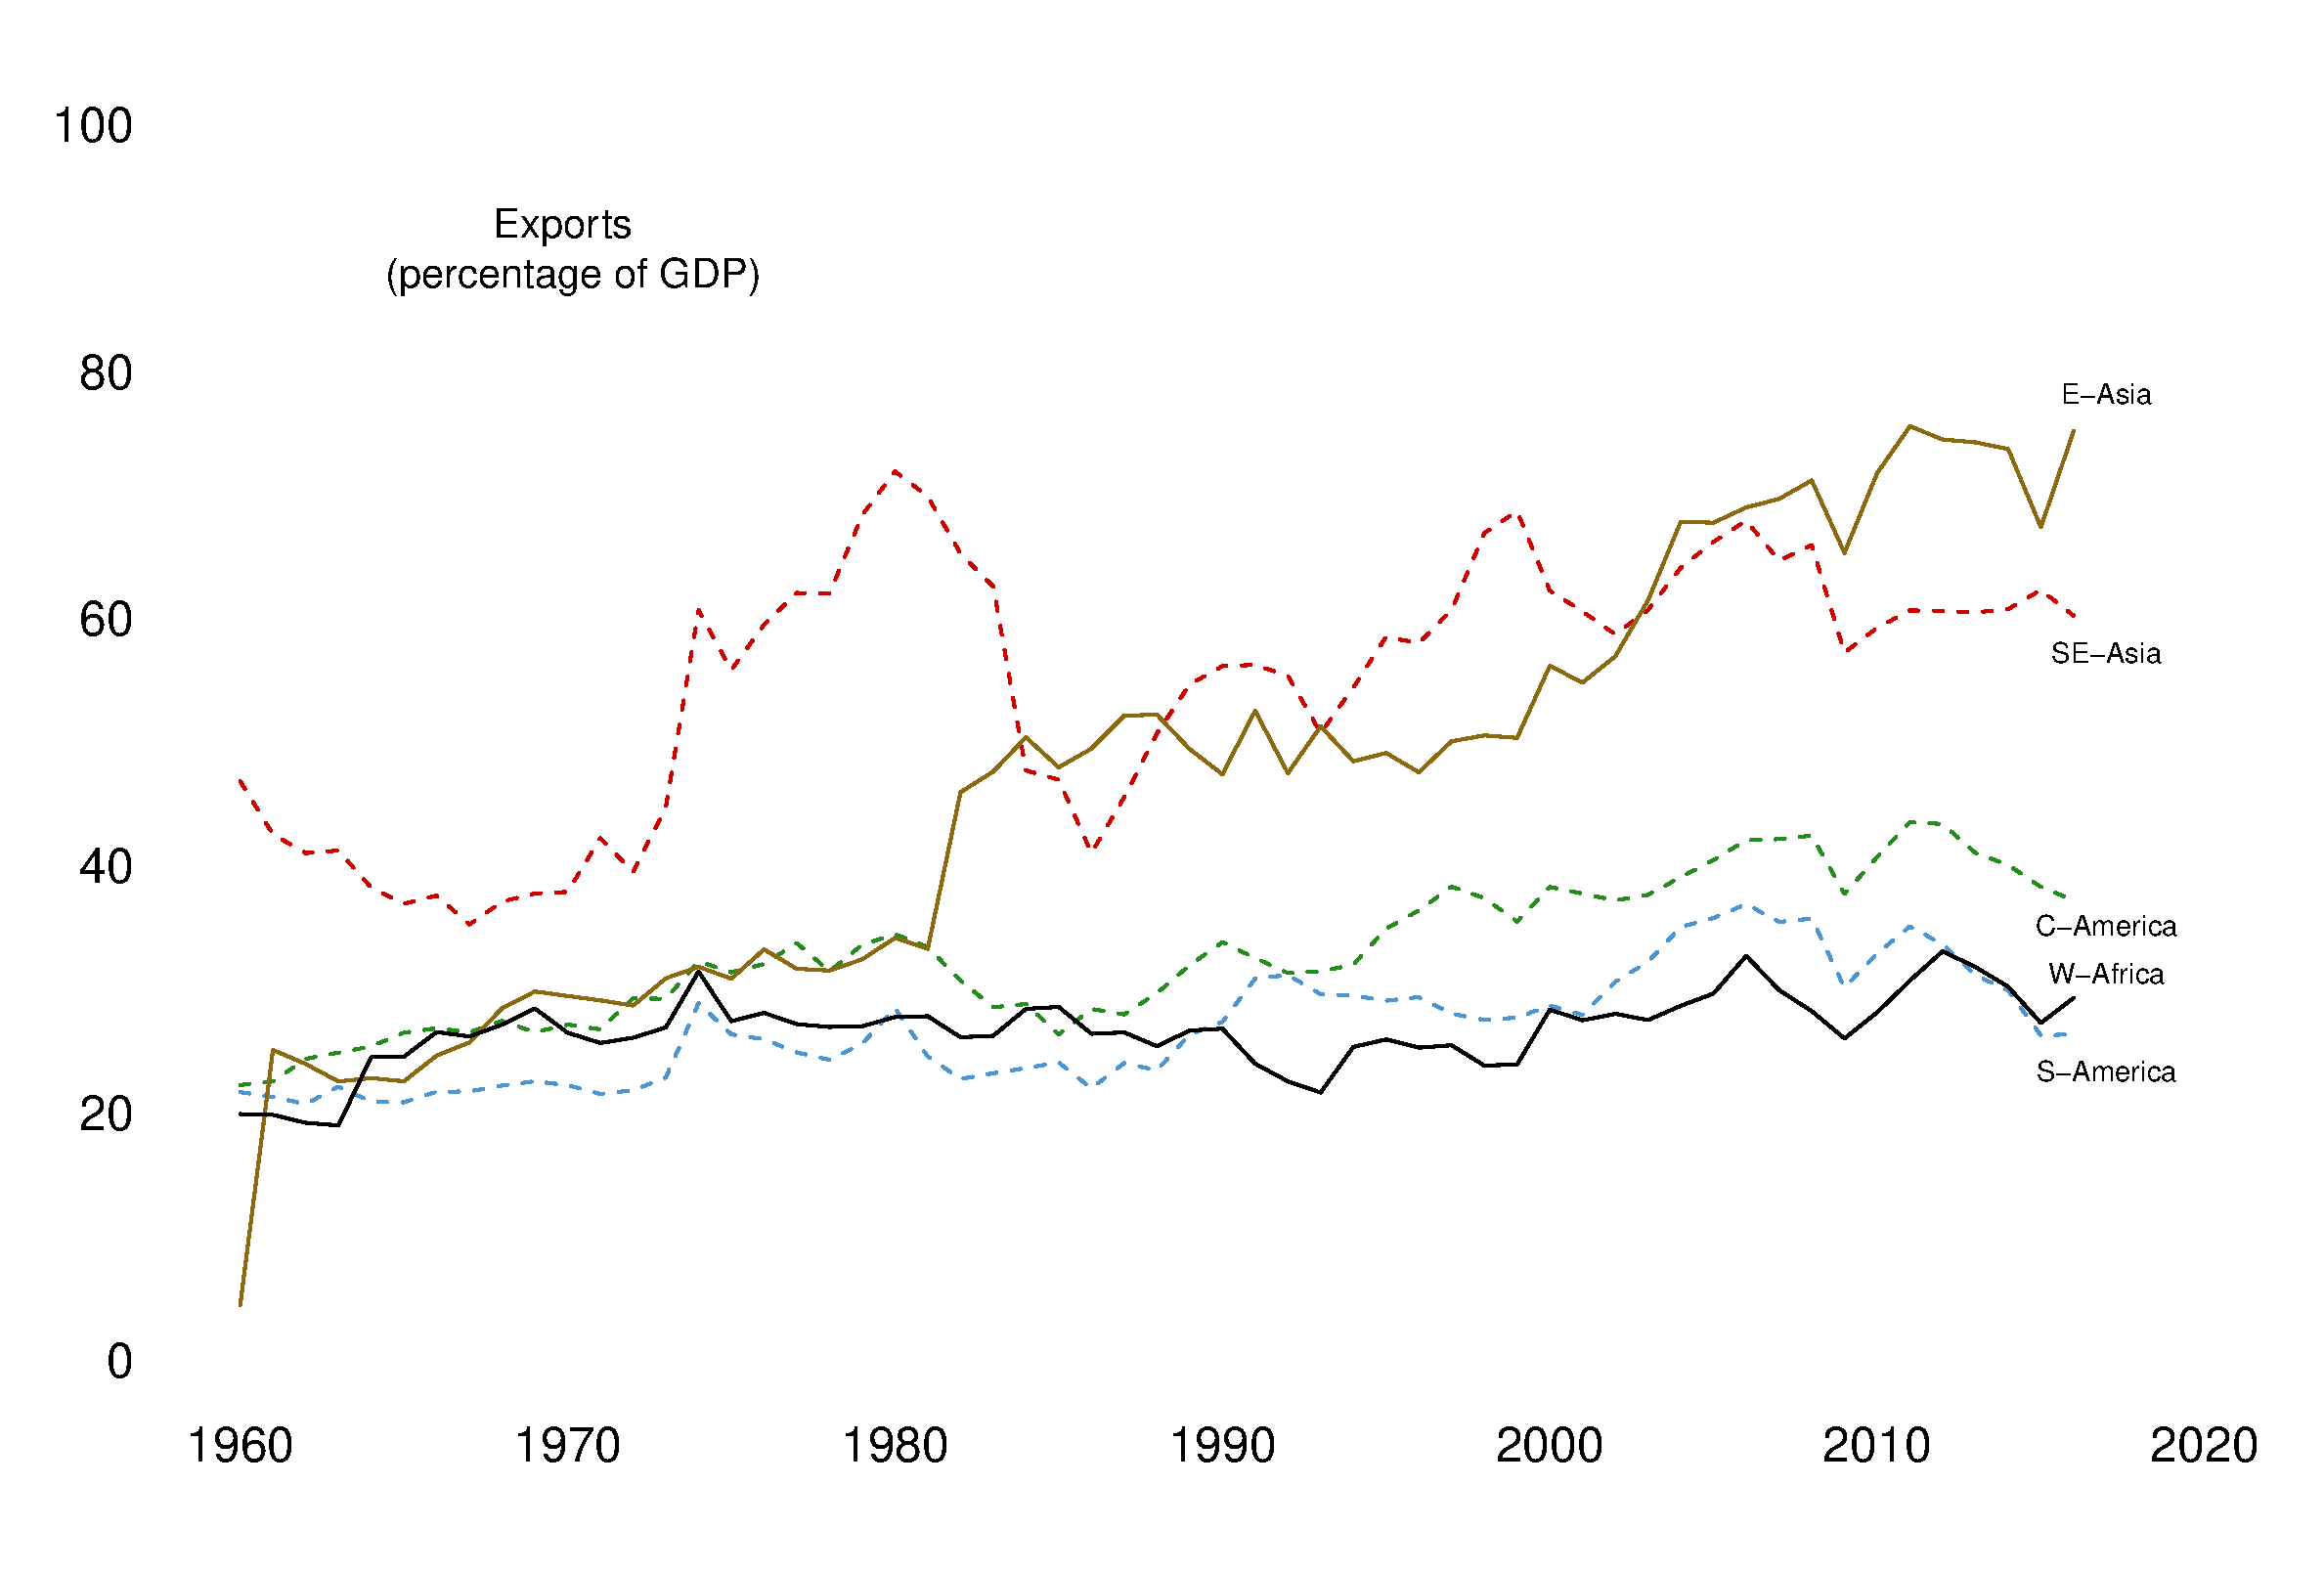
\includegraphics[scale=.3]{exports.eps}
  \end{figure}
\end{frame}
%--------------------------------------

%--------------------------------------
\begin{frame}
  \begin{figure}
    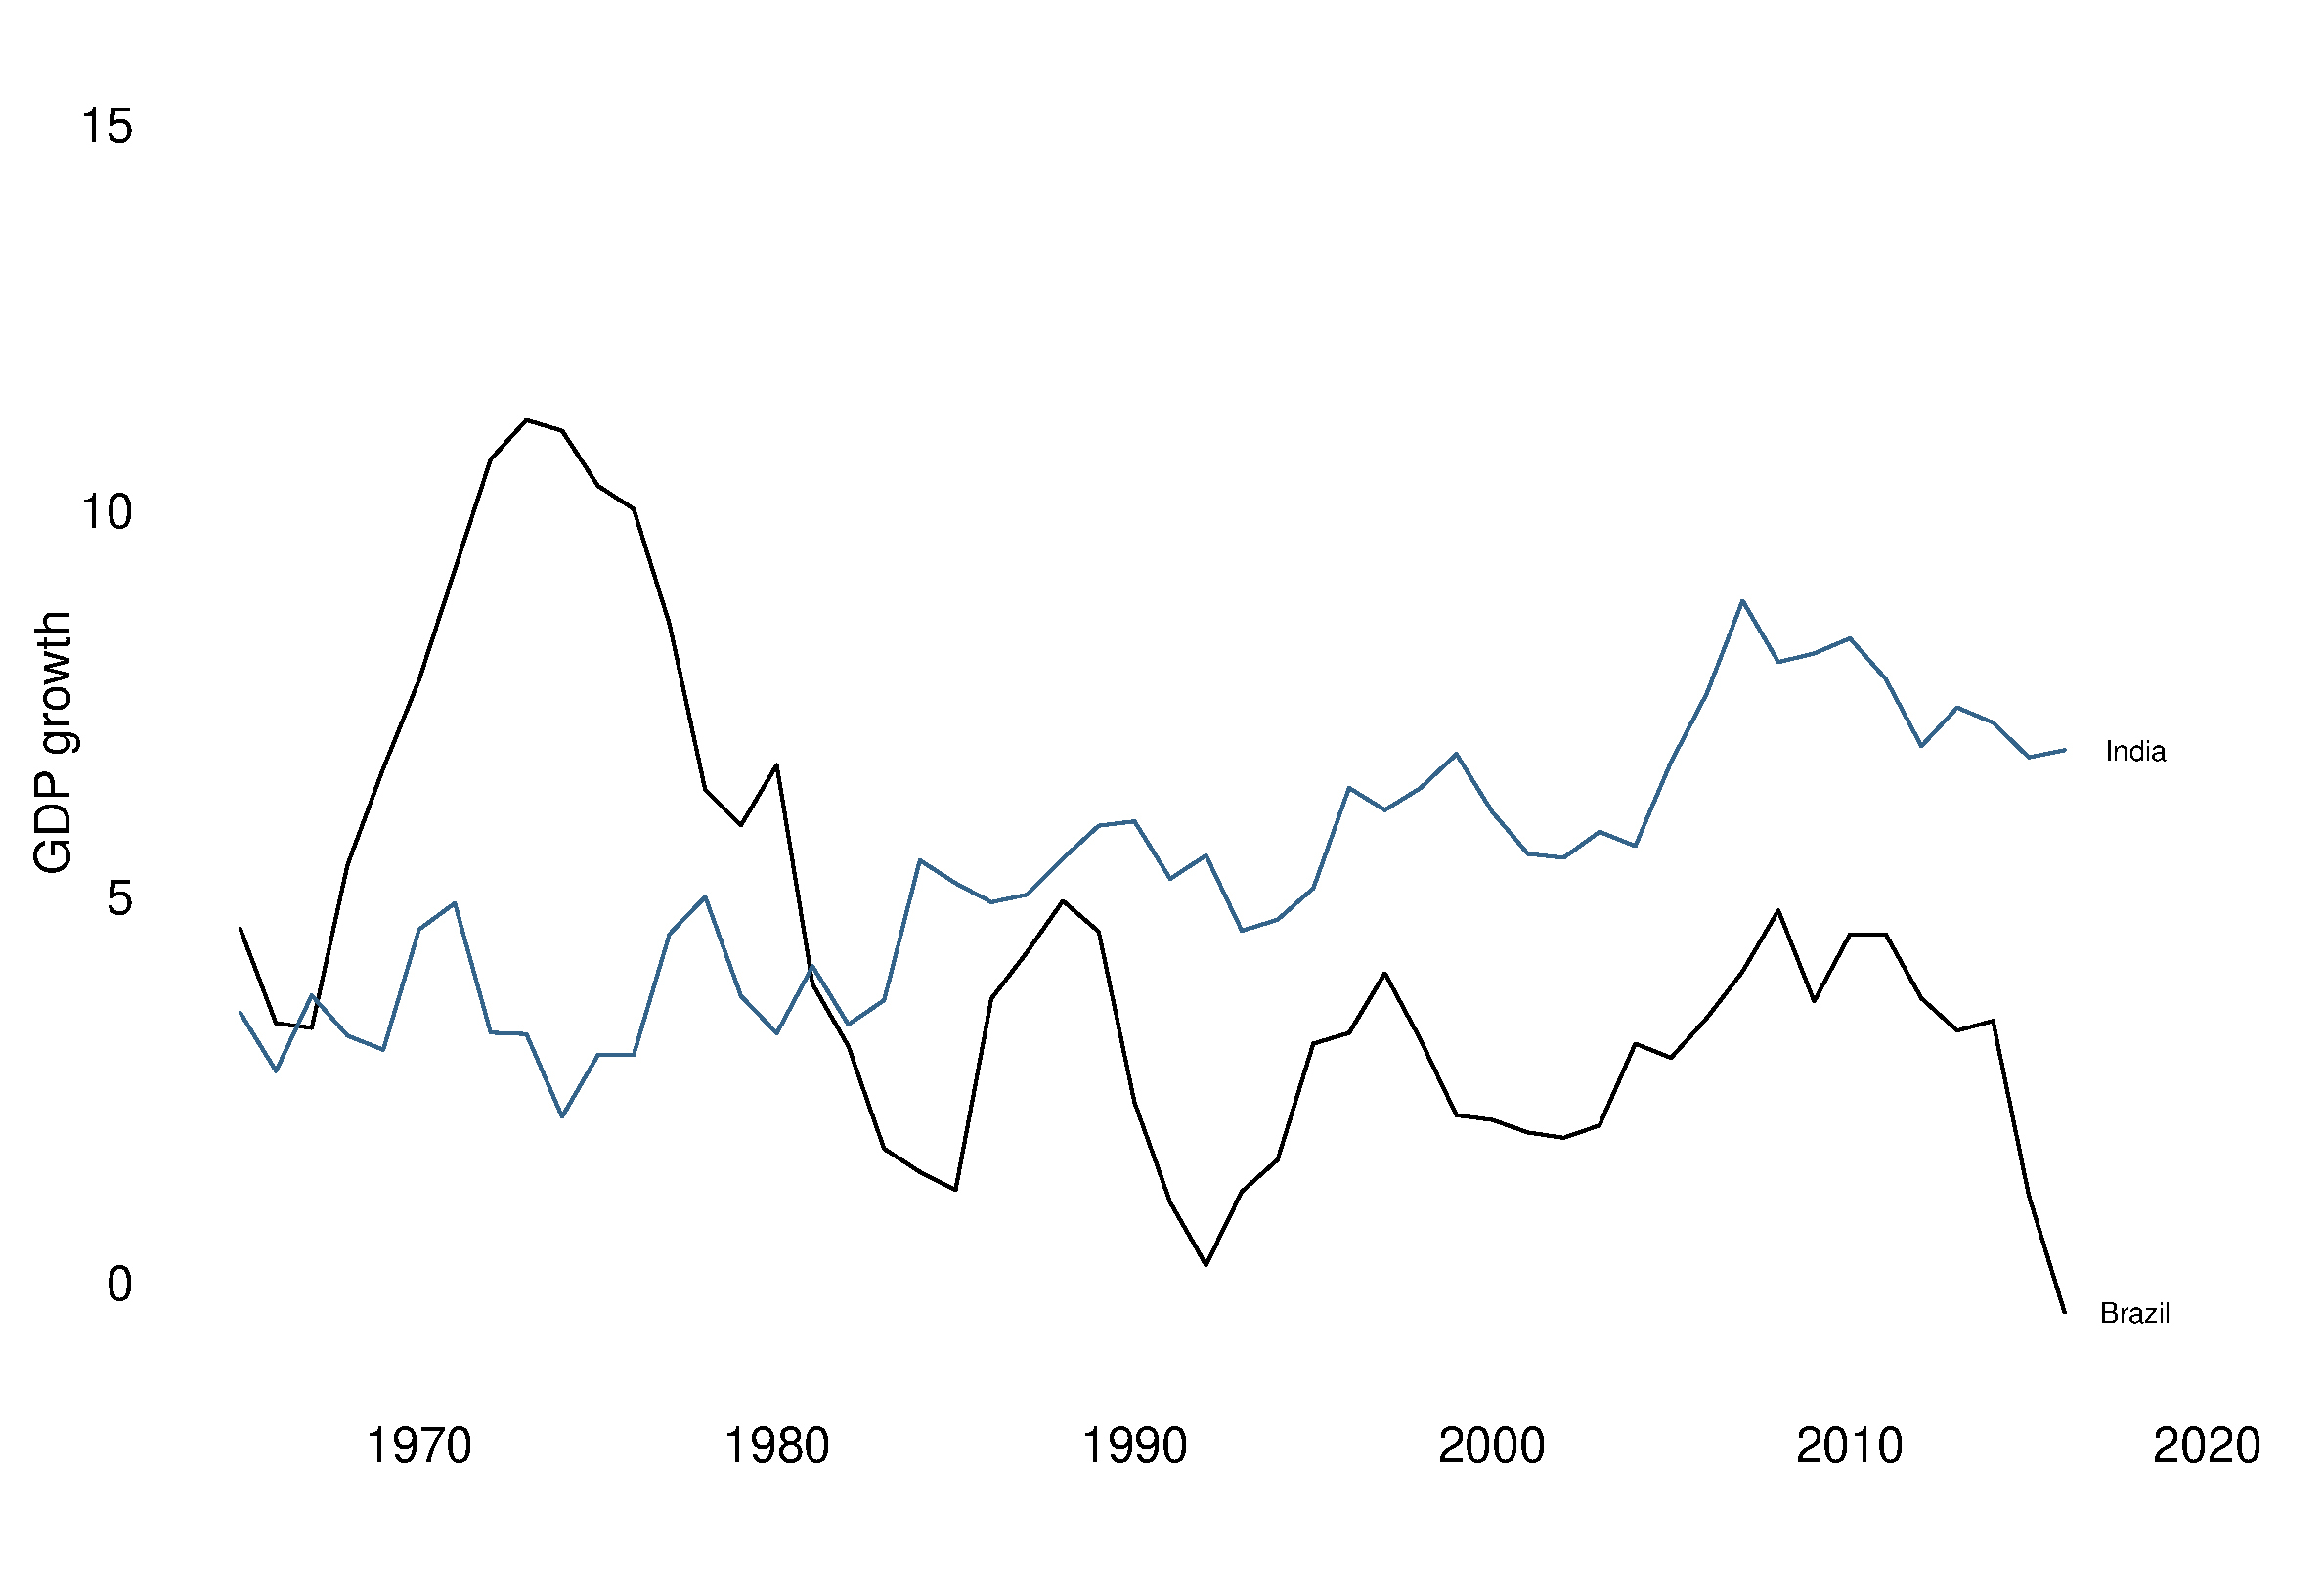
\includegraphics[scale=.3]{bra_ind.eps}
  \end{figure}
\end{frame}
%--------------------------------------

%--------------------------------------
\begin{frame}
  \begin{figure}
    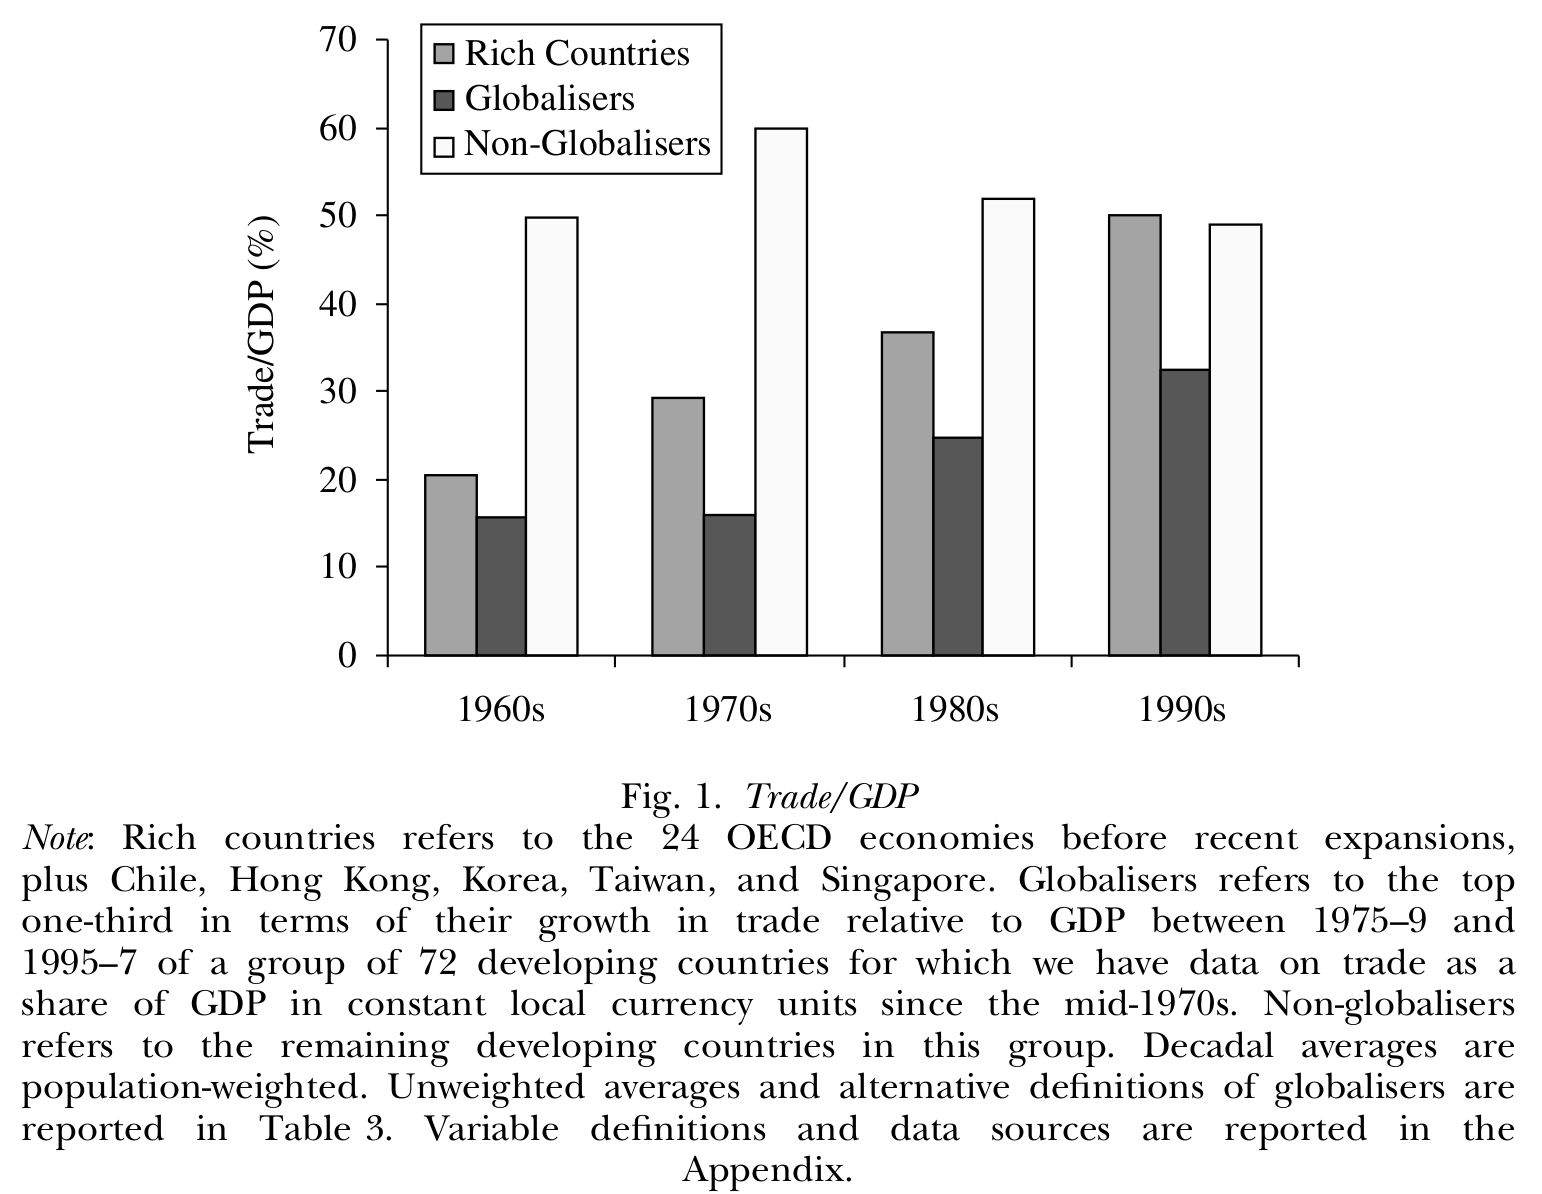
\includegraphics[scale=.6]{dollar_kraay.png}
  \end{figure}
  Dollar \& Kraay, 2004, "Trade, Growth, and Poverty"
\end{frame}
%--------------------------------------

%--------------------------------------
\begin{frame}
  \begin{figure}
    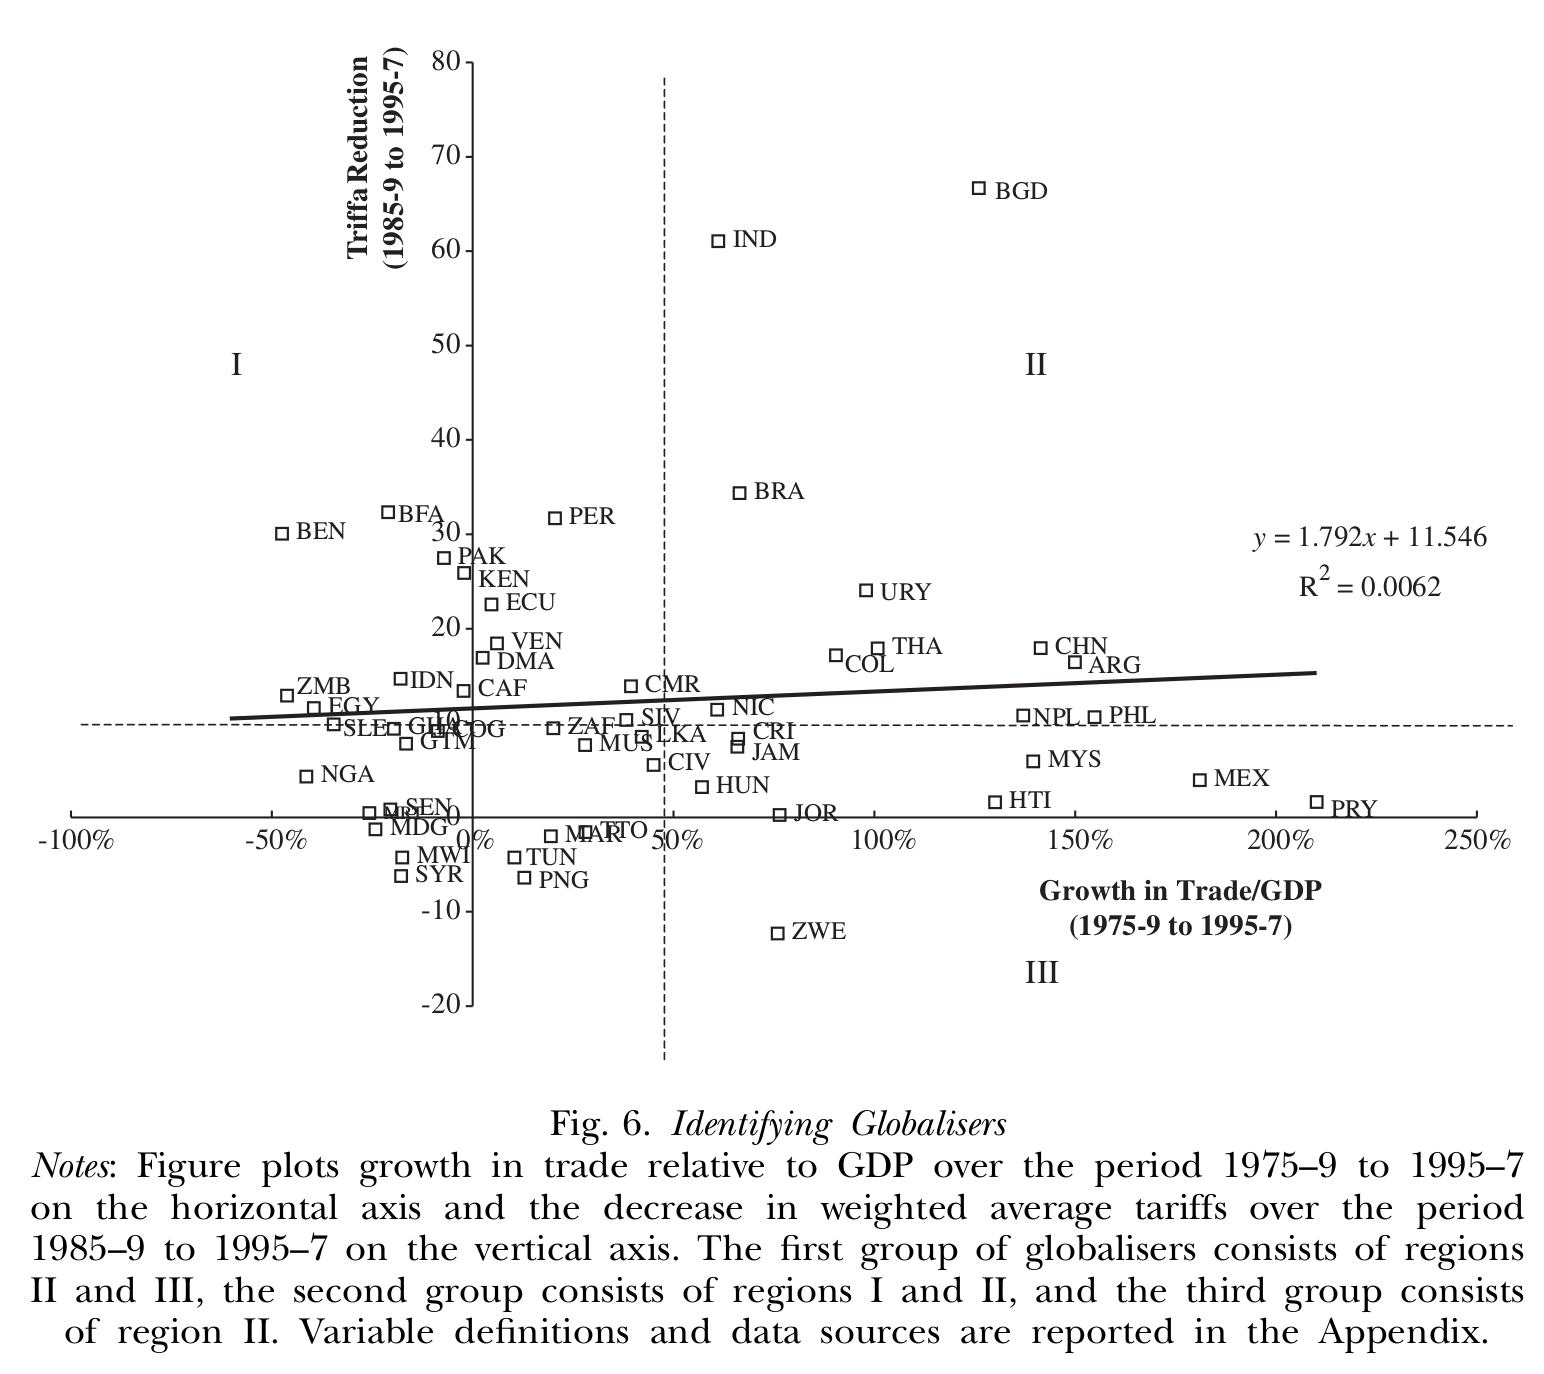
\includegraphics[scale=.6]{dollar_kraay2.png}
  \end{figure}
  Dollar \& Kraay, 2004, "Trade, Growth, and Poverty"
\end{frame}
%--------------------------------------

%--------------------------------------
\begin{frame}
  Interesting example in terms of the effect of trade liberalisation is Mexico
  \begin{itemize}
    \item Throughout 1950-60s high tariff barriers
    \item Produced little for exports, main export product was oil
  \end{itemize}
  \medskip
  From 1980s onwards process of trade liberalisation
  \begin{itemize}
    \item 1985-88, removal of tariffs and quotas
    \item 1994, joined NAFTA
  \end{itemize}
  \medskip
  Mexico is 13th largest exporter in the world.
\end{frame}
%--------------------------------------

%--------------------------------------
\begin{frame}
  \begin{figure}
    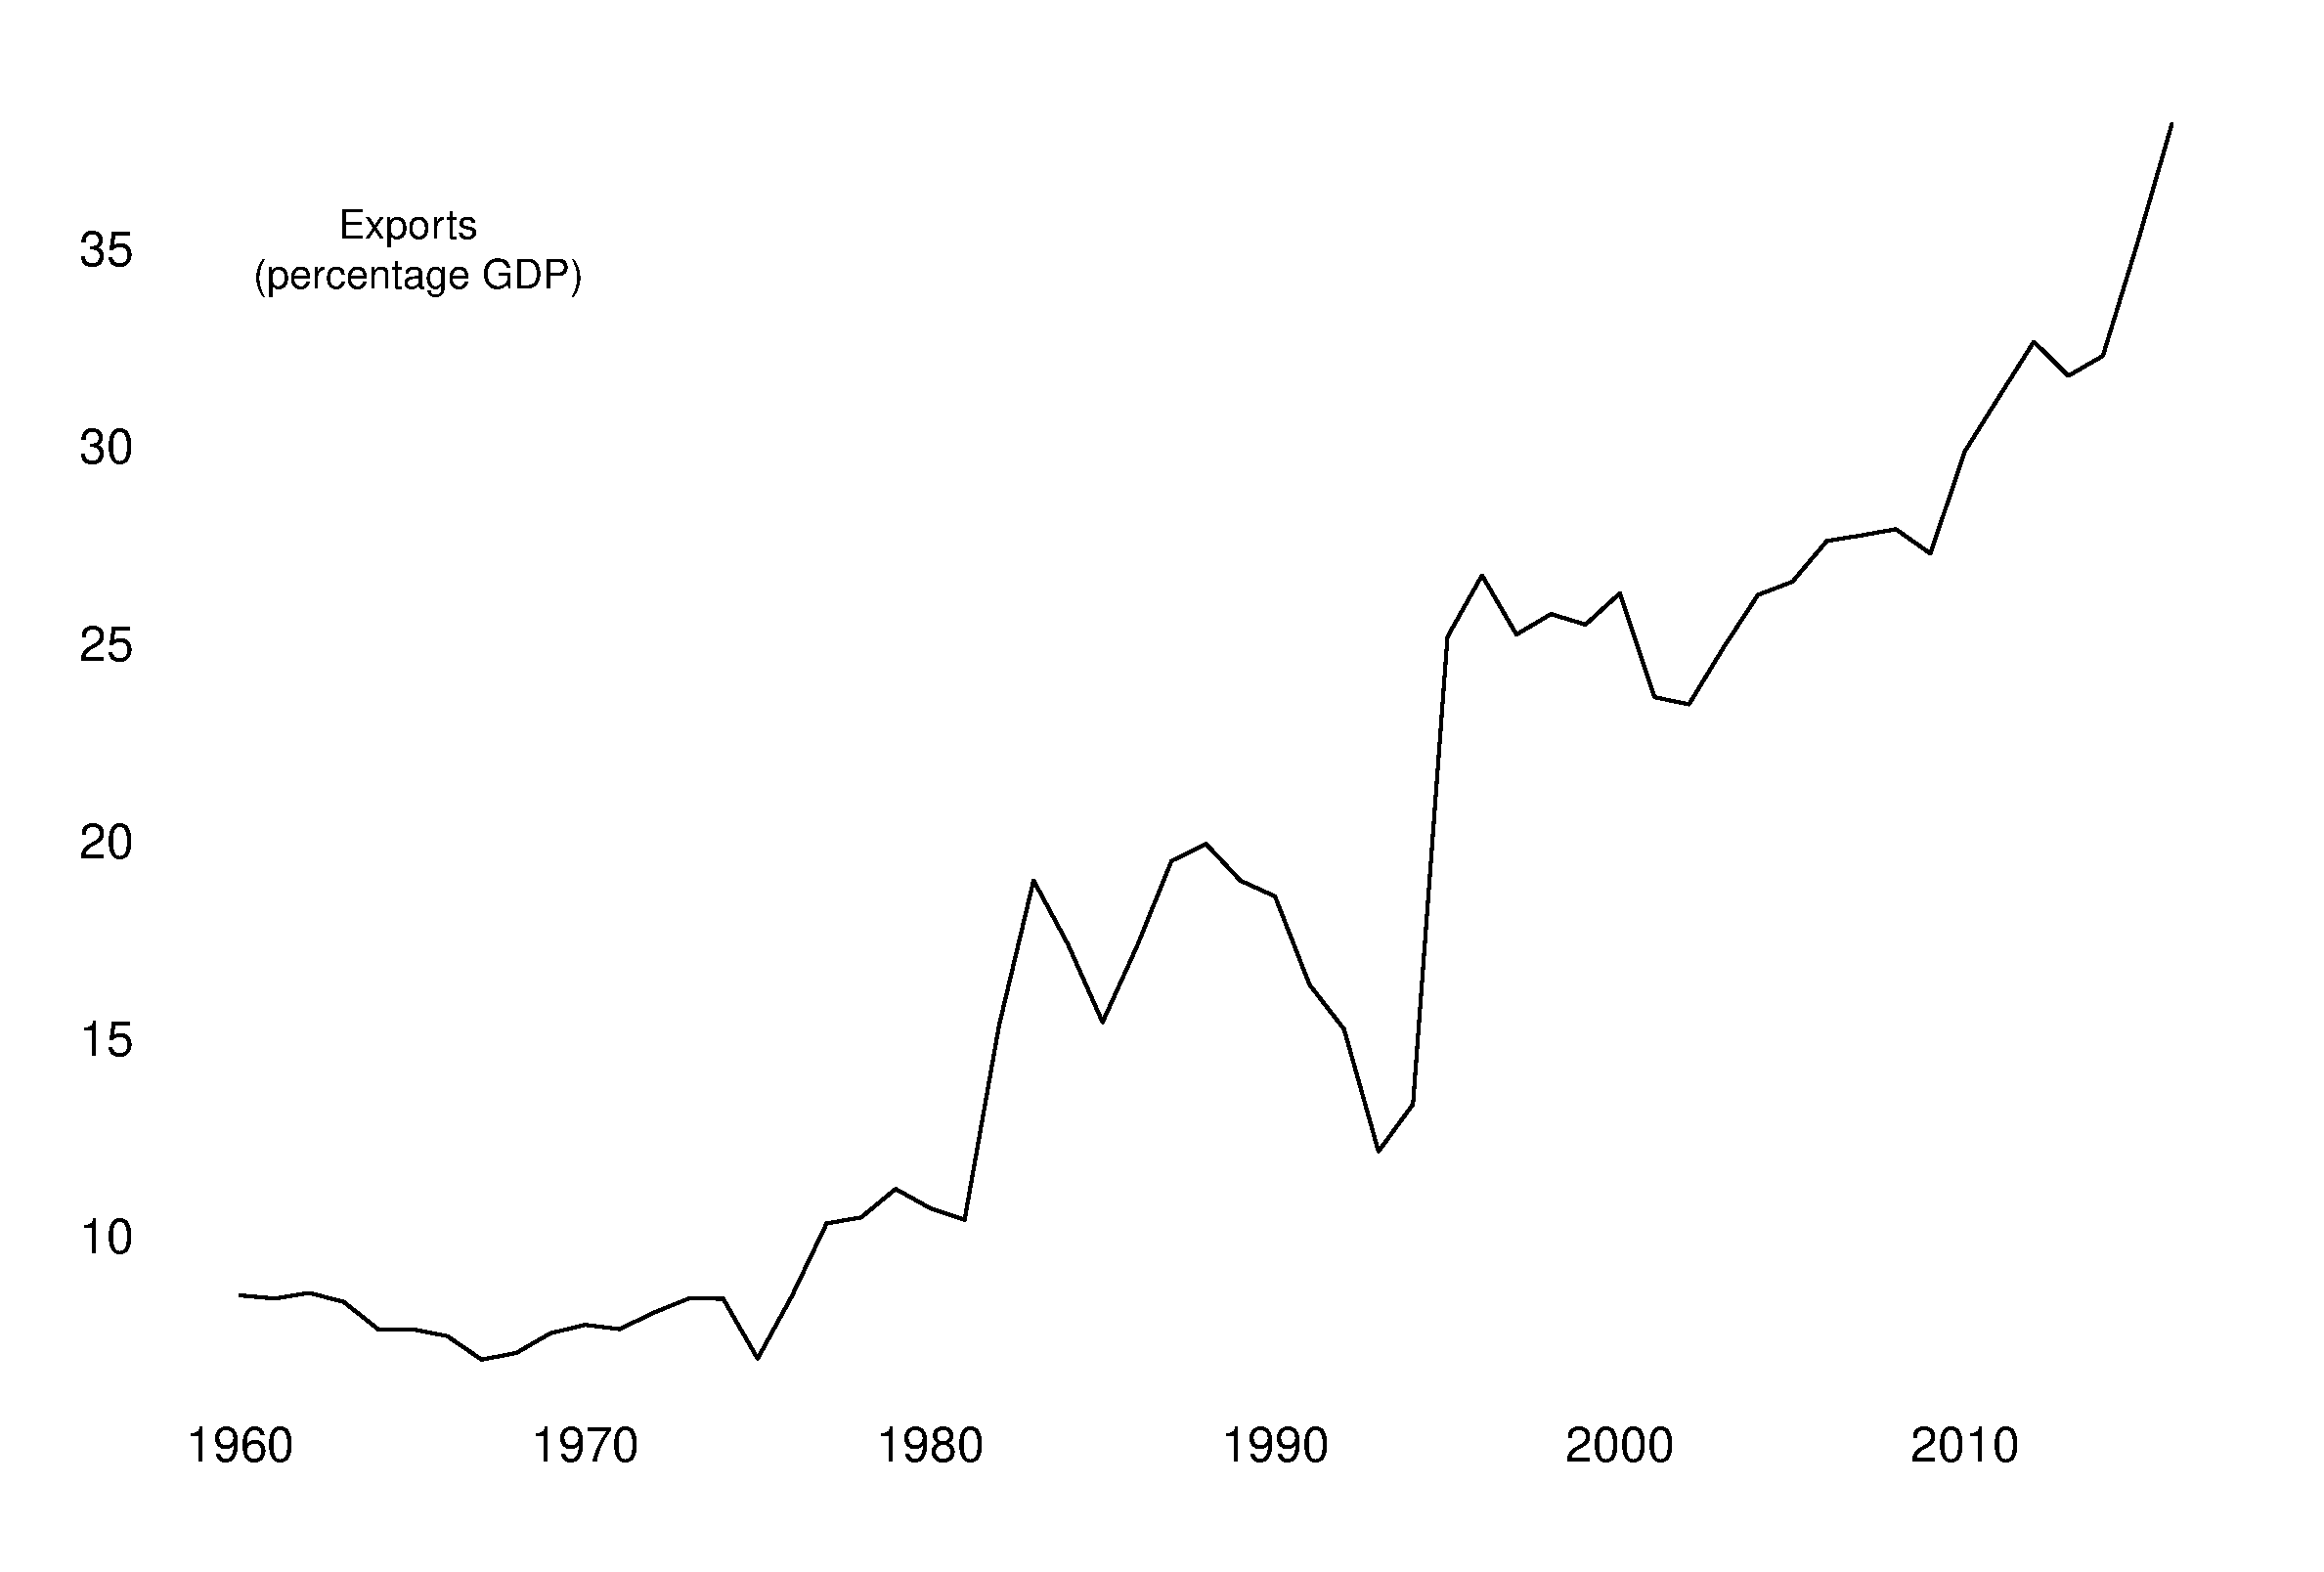
\includegraphics[scale=.3]{mexico1.eps}
  \end{figure}
\end{frame}
%--------------------------------------

%--------------------------------------
\begin{frame}
  \begin{figure}
    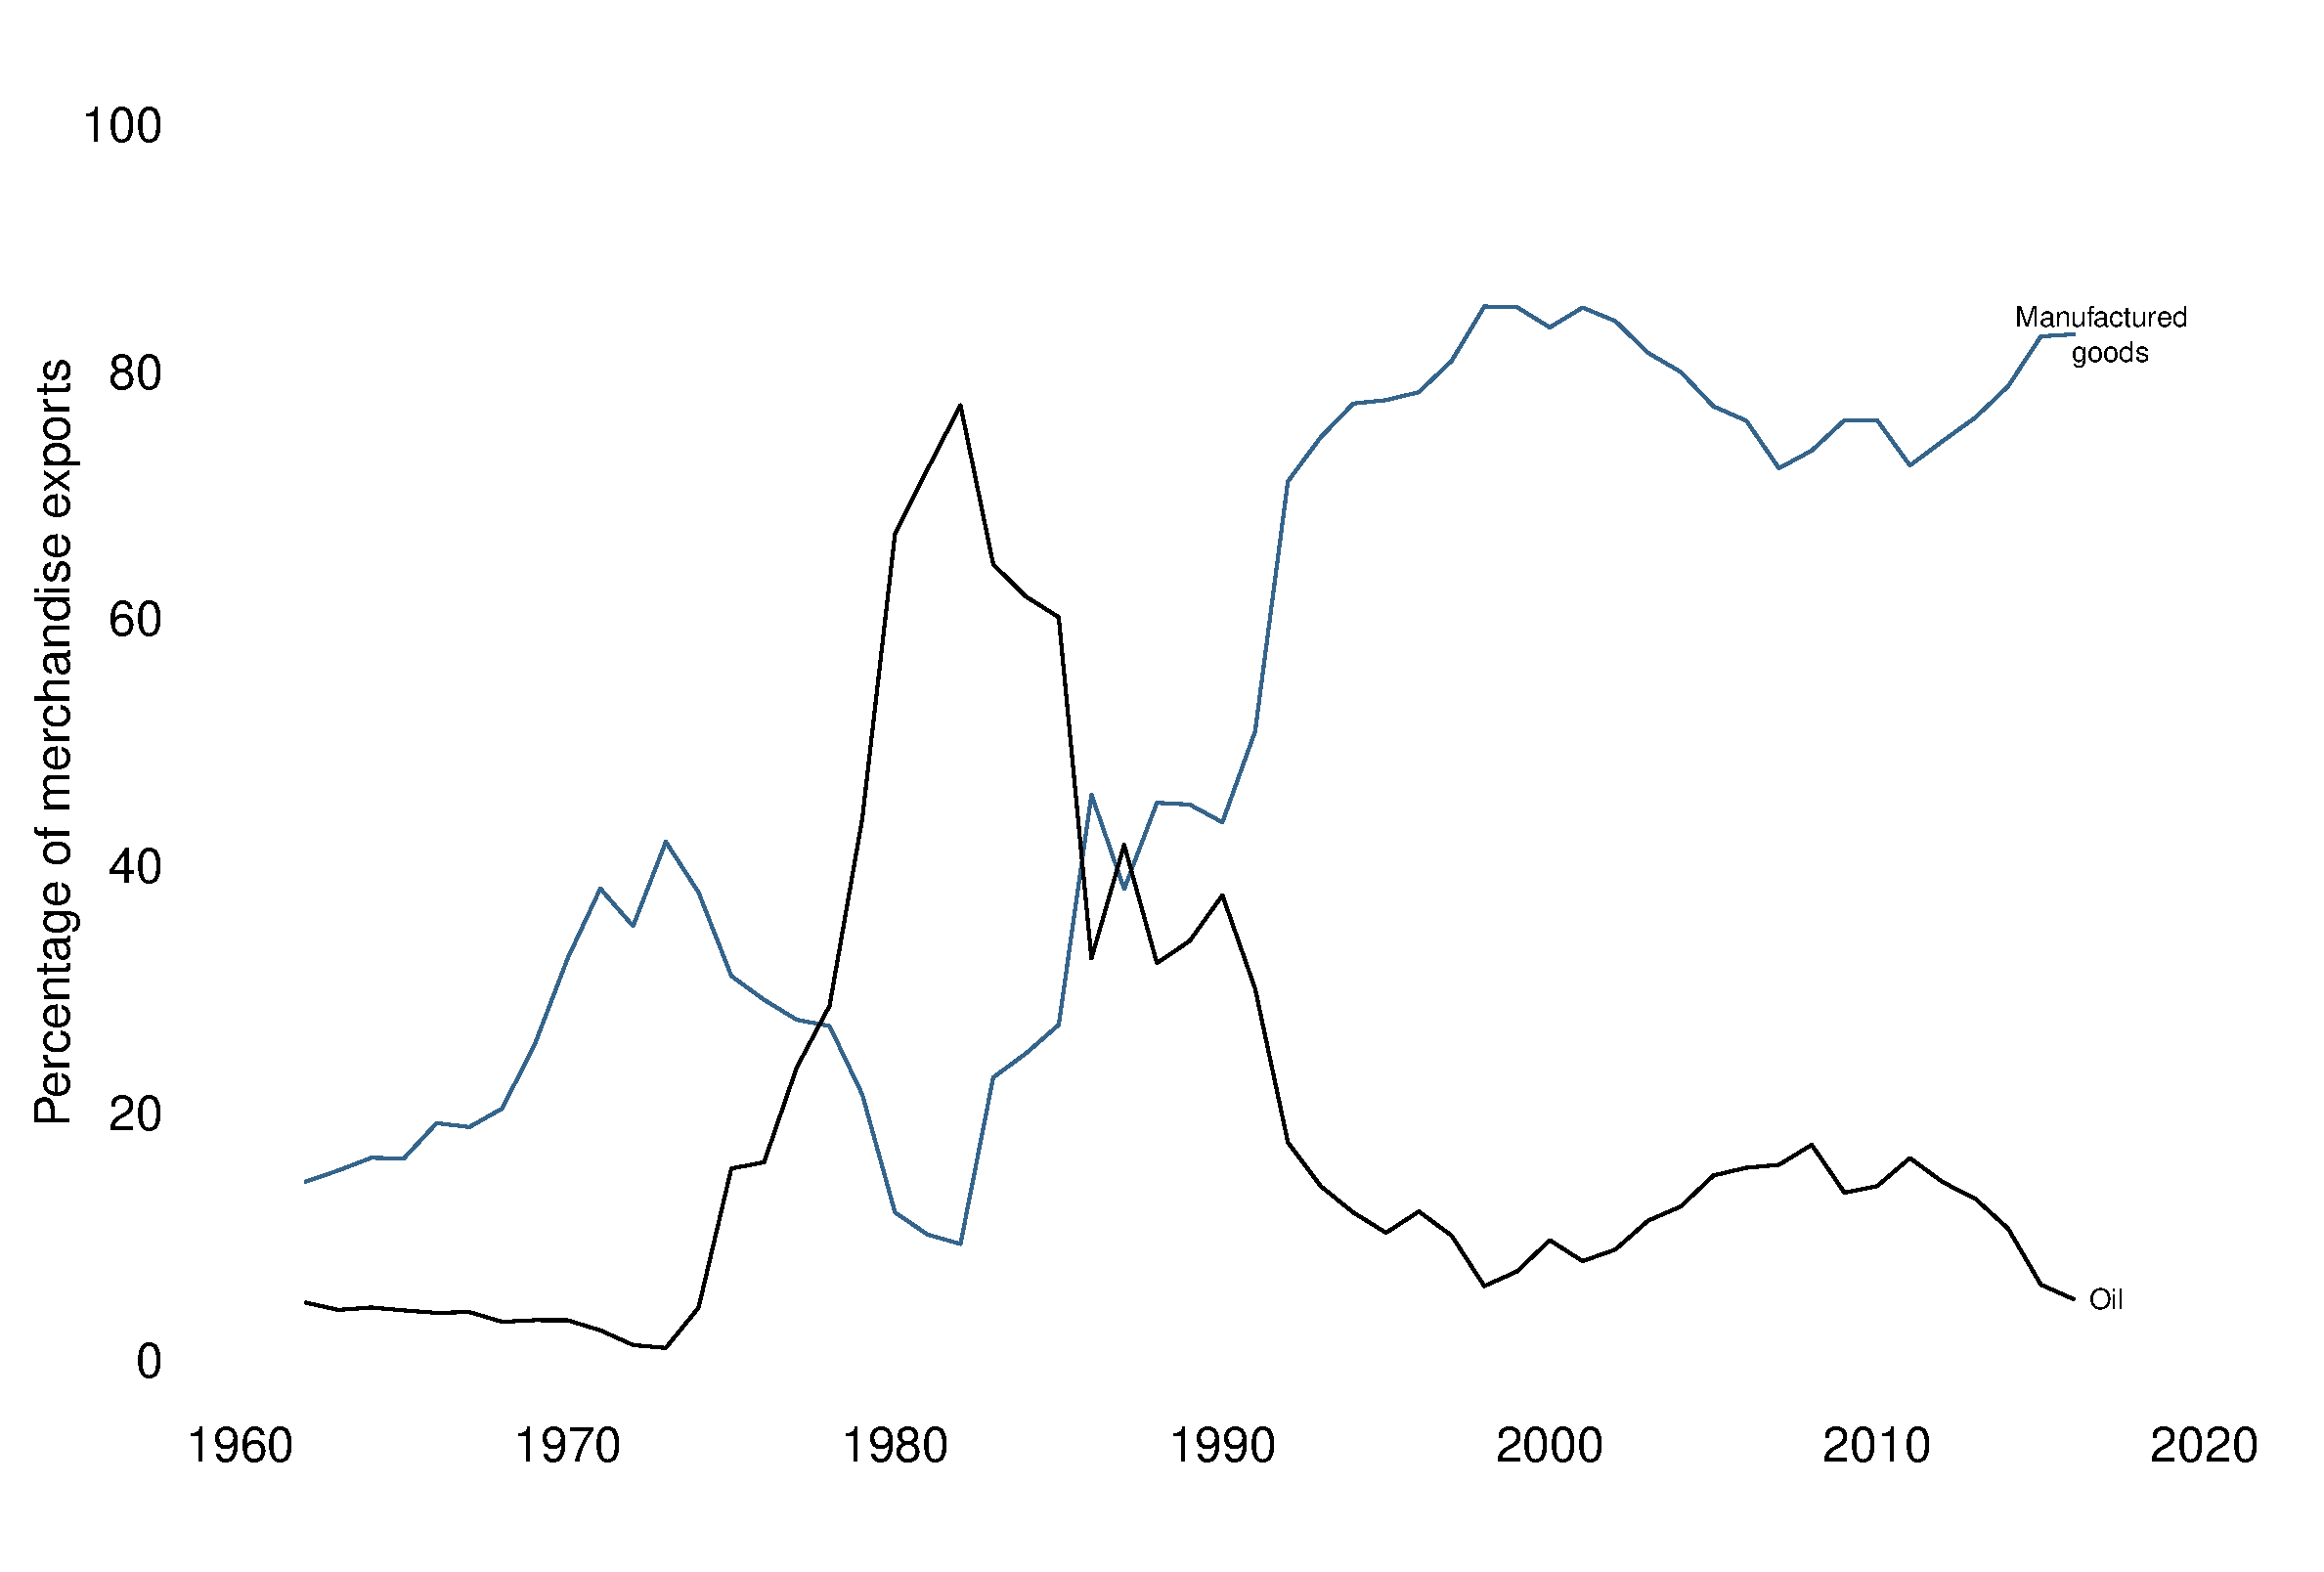
\includegraphics[scale=.3]{mexico2.eps}
  \end{figure}
\end{frame}
%--------------------------------------

%--------------------------------------
\begin{frame}
  \begin{figure}
    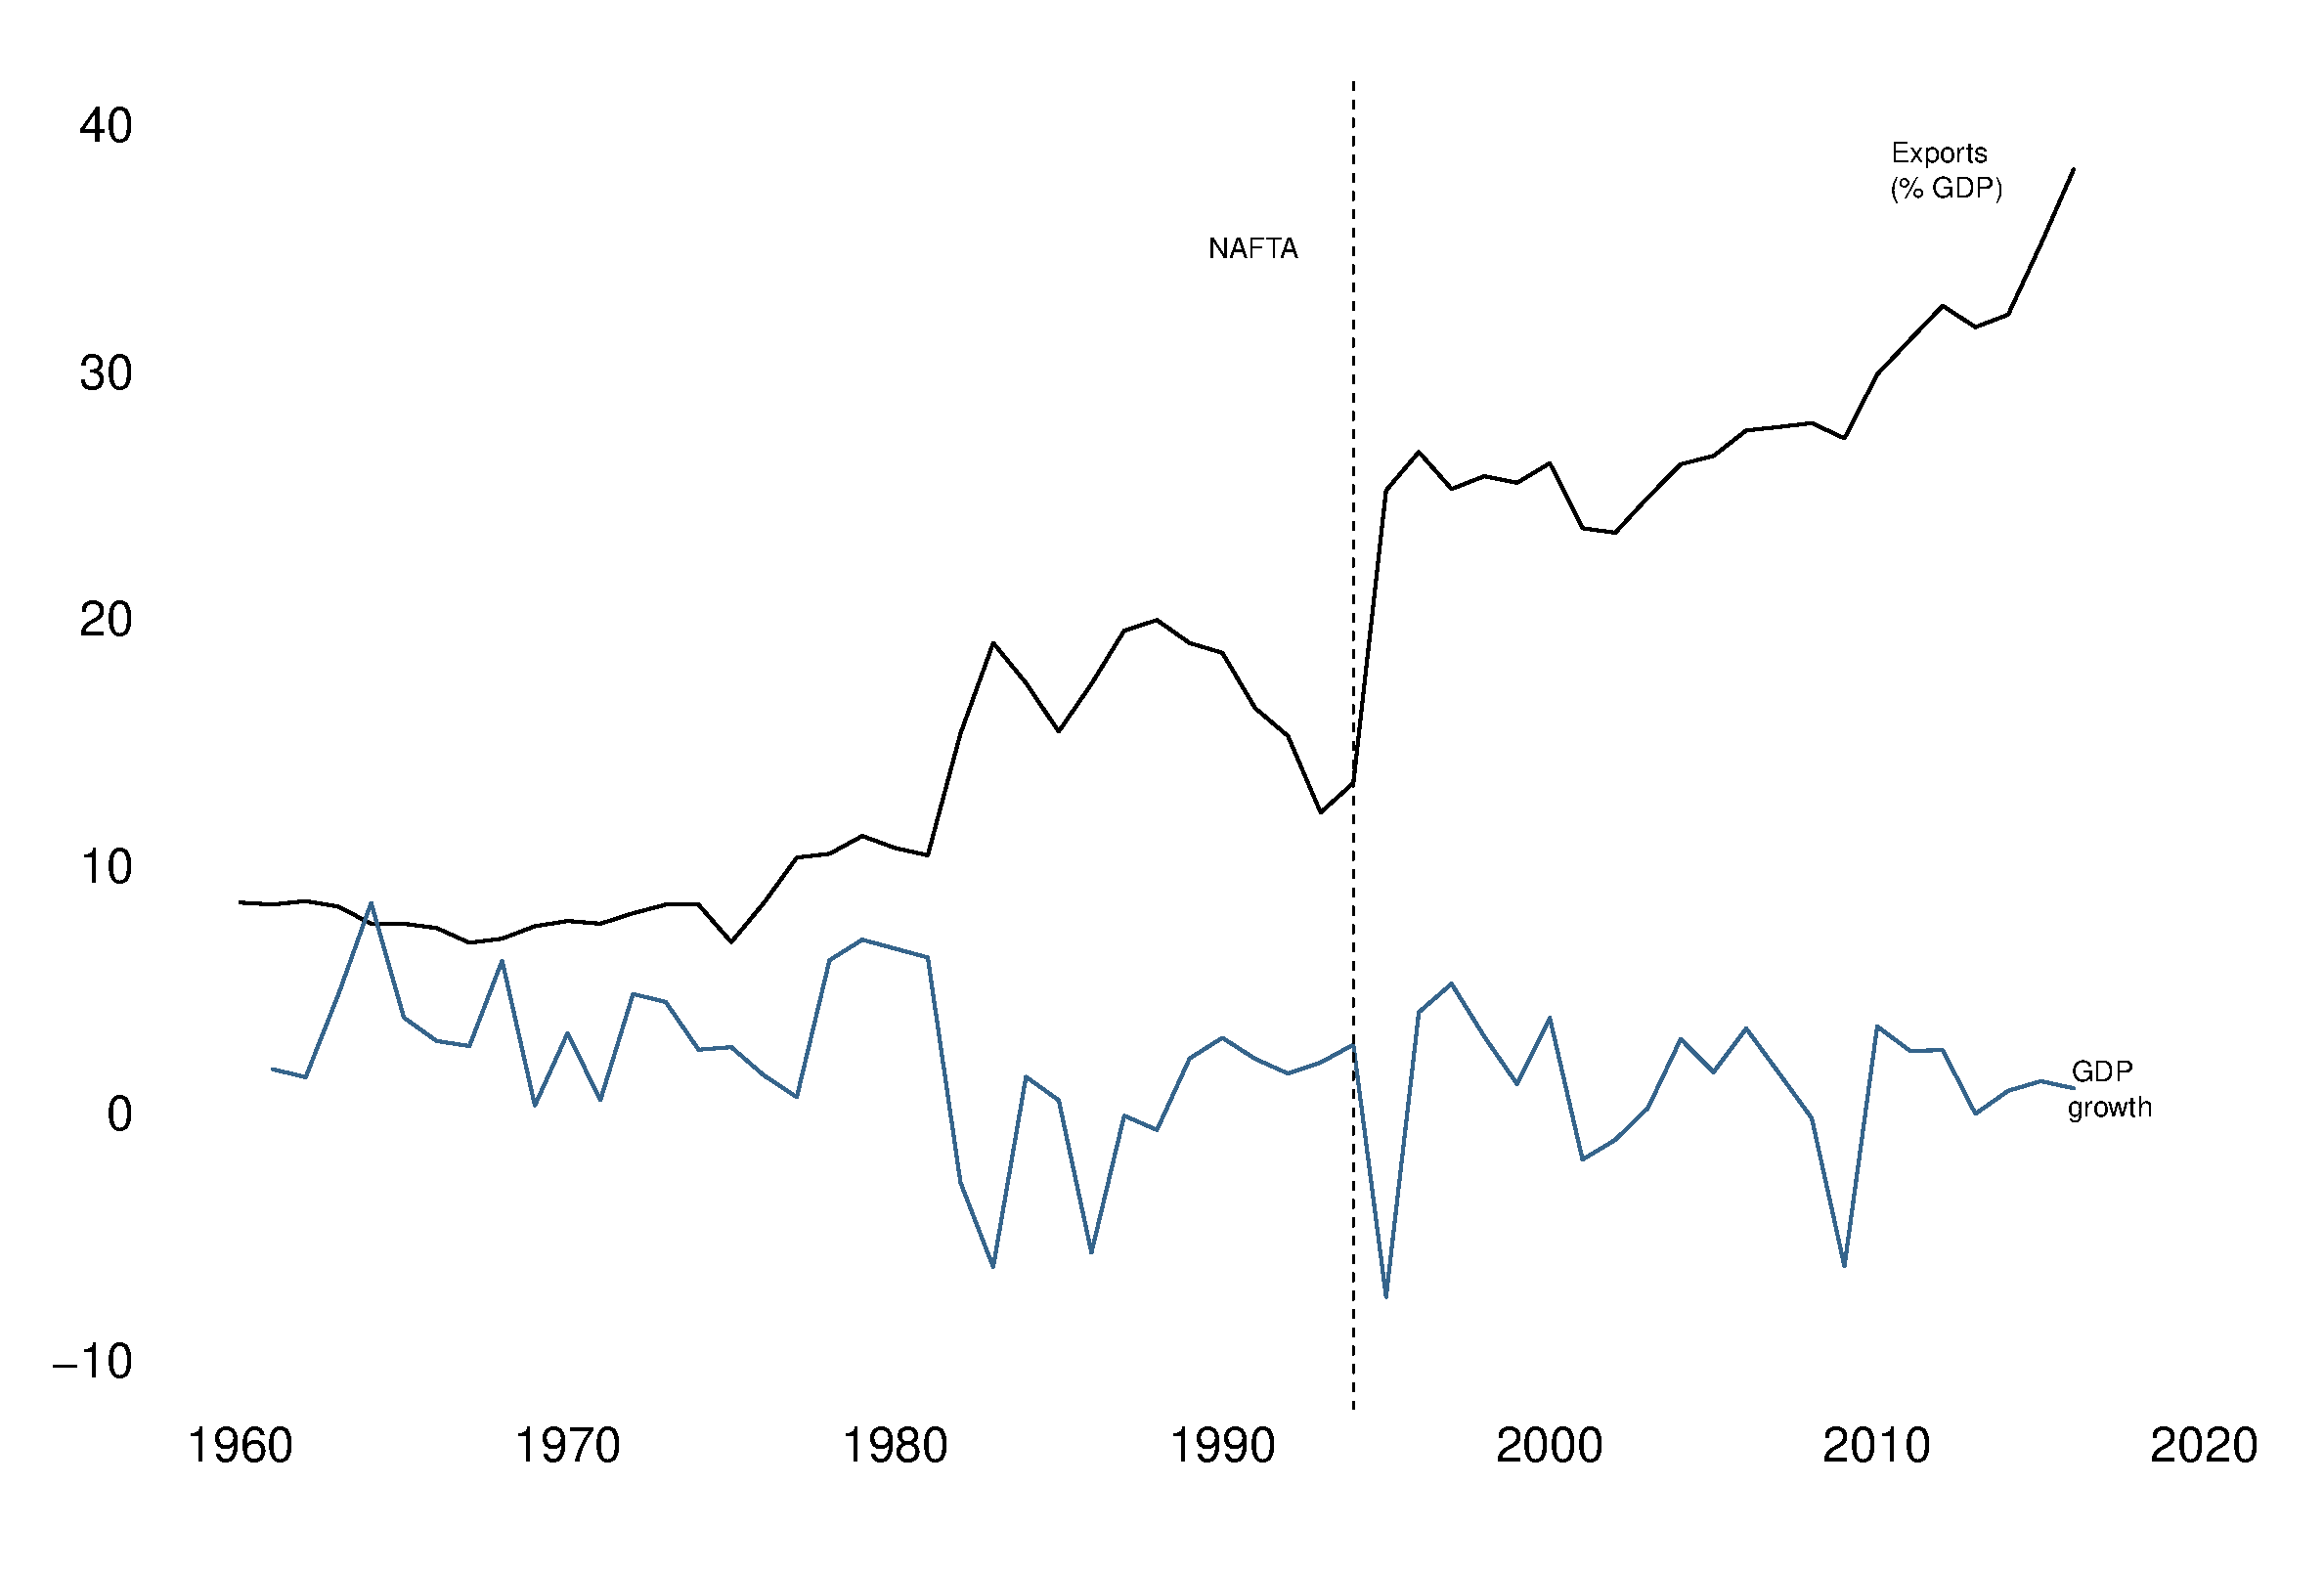
\includegraphics[scale=.3]{mexico3.eps}
  \end{figure}
\end{frame}
%--------------------------------------

%--------------------------------------
\begin{frame}
 One issue is that developed countries often use agriculatural tariffs and subsidies which hurt developing countries
 \begin{itemize}
   \item EU's Common Agricultural Policy
   \item Cotton and Sugar in the USA
 \end{itemize}
\end{frame}
%--------------------------------------

%--------------------------------------
\begin{frame}
 What are for example the effects of export subsidies for foreign countries?
 \begin{itemize}
   \item Decrease world prices
 \end{itemize}
 \medskip
 This will be great for foreign consumers but not so much for foreign producers
 \begin{itemize}
   \item Helps net-exporters but hurts net-importers
 \end{itemize}
\end{frame}
%--------------------------------------

%--------------------------------------
\begin{frame}
  \begin{figure}
    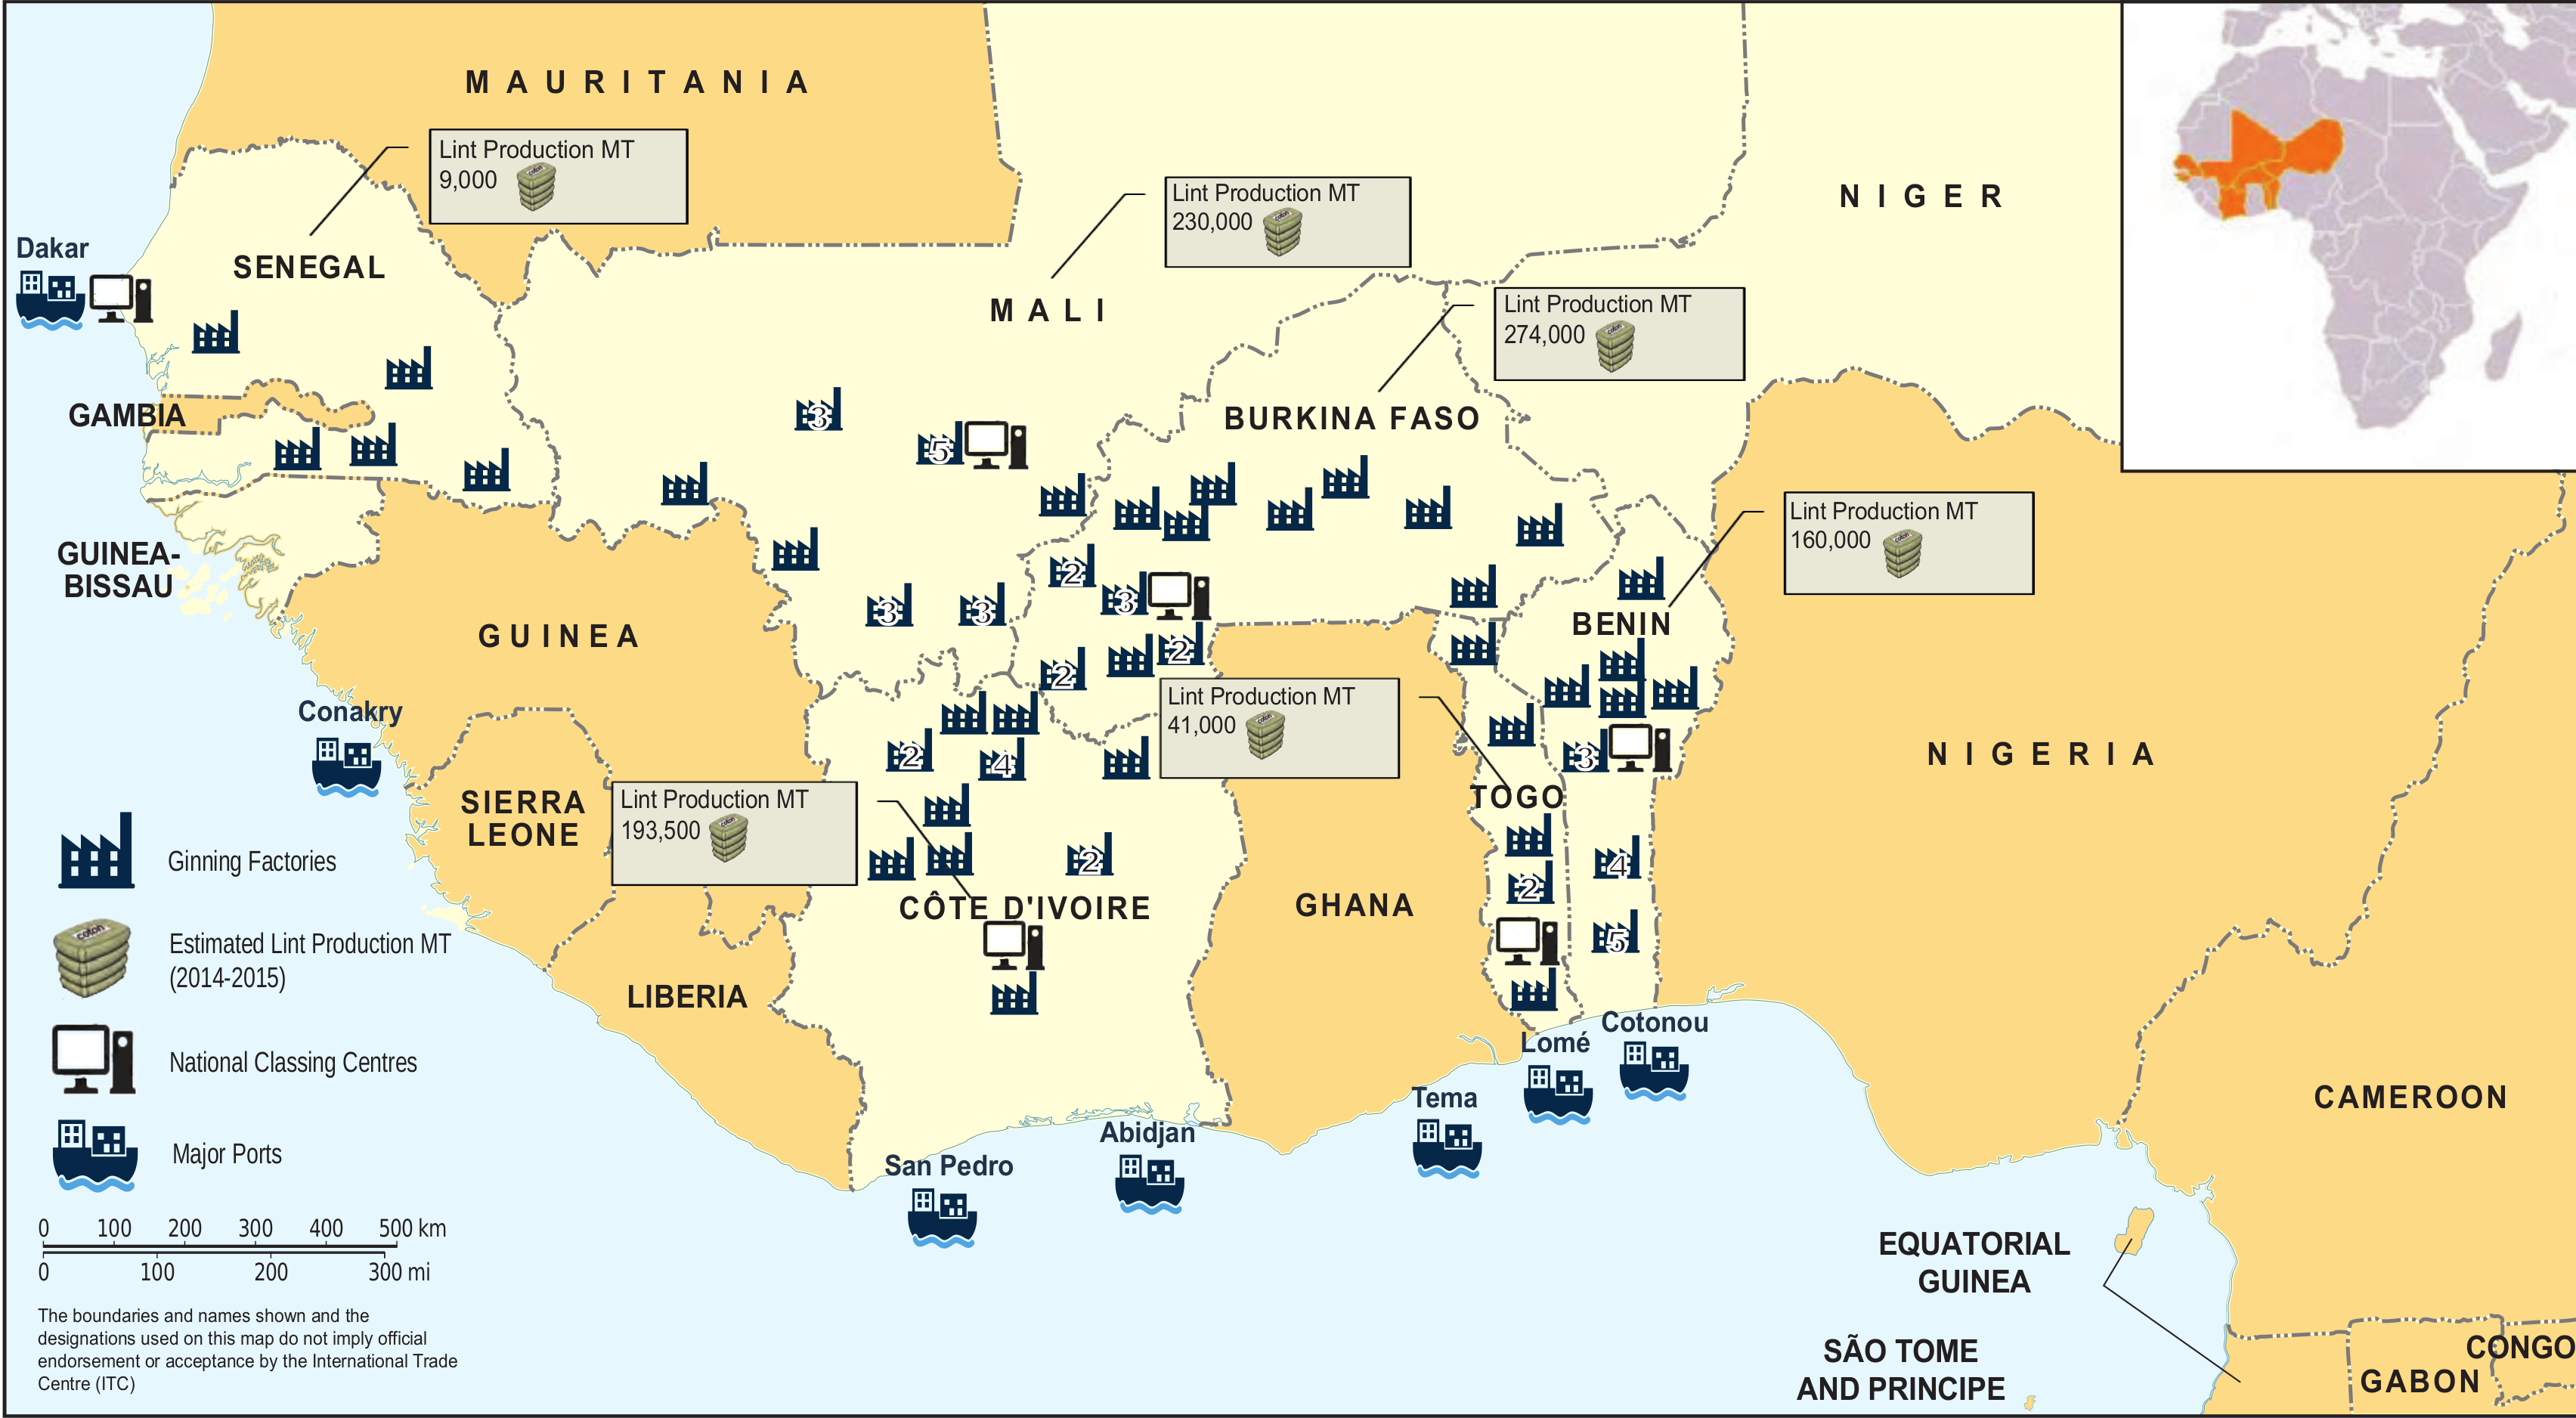
\includegraphics[scale=.35]{cotton.png}
  \end{figure}
\end{frame}
%--------------------------------------

%--------------------------------------
\begin{frame}
 Consider cotton, the production cost for which are three times lower in West-Africa than in the USA
 \begin{itemize}
   \item US farmers receive 4B USD in subsidies, a year
 \end{itemize}
 \medskip
 From 1998 to 2001 US output grew by 40\%, exports by 50\%, decreasing world prices to record low
\end{frame}
%--------------------------------------

%--------------------------------------
\begin{frame}
 Would developing countries be better off if rich nations stopped subsiding their agricultural sectors?
 Probably not.
 \begin{itemize}
   \item Developing countries are predominantly net-importers of agricultural goods   
 \end{itemize}
 \medskip
 Poor will be hurt. 
\end{frame}
%--------------------------------------

%--------------------------------------
\begin{frame}
  There has been a strong increase in South-South trade
  \begin{itemize}
    \item Developing countries accounted for 50\% of increase in global exports between 1995-2012
    \item Account for 45\% of global GDP
    \item Fuels and manufactured goods account for 25 and 19\% of trade
  \end{itemize}
  \medskip
  This increase in trade is mainly driven by the development of Asian and American economies.
\end{frame}
%--------------------------------------

%--------------------------------------
\begin{frame}{Source: UNCTAD}
  \begin{figure}
    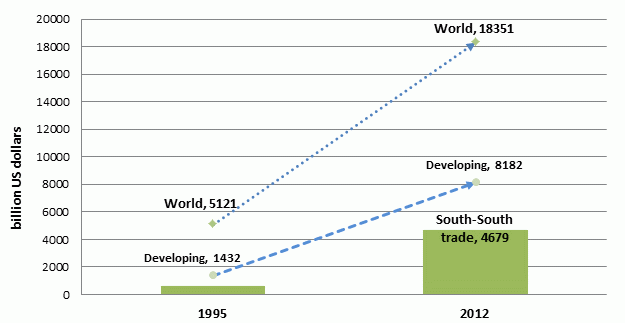
\includegraphics[scale=.5]{unctad.png}
  \end{figure}
\end{frame}
%--------------------------------------

%------------------------------------------------------------------------------
\end{document}
